% !TEX encoding = UTF-8 Unicode
% !TEX root = thesis-ex.tex

A description of the analysis procedure to reconstruct the $\Dptr$ distribution, along with the derivation and application of the various corrections is presented in the following sections.
The analysis structure is illustrated by the diagram in Figure~\ref{fig:analysis_flow} where each part of the analyses is described in a separate subsection and can be summarized as follows: 




\begin{figure}
\centering
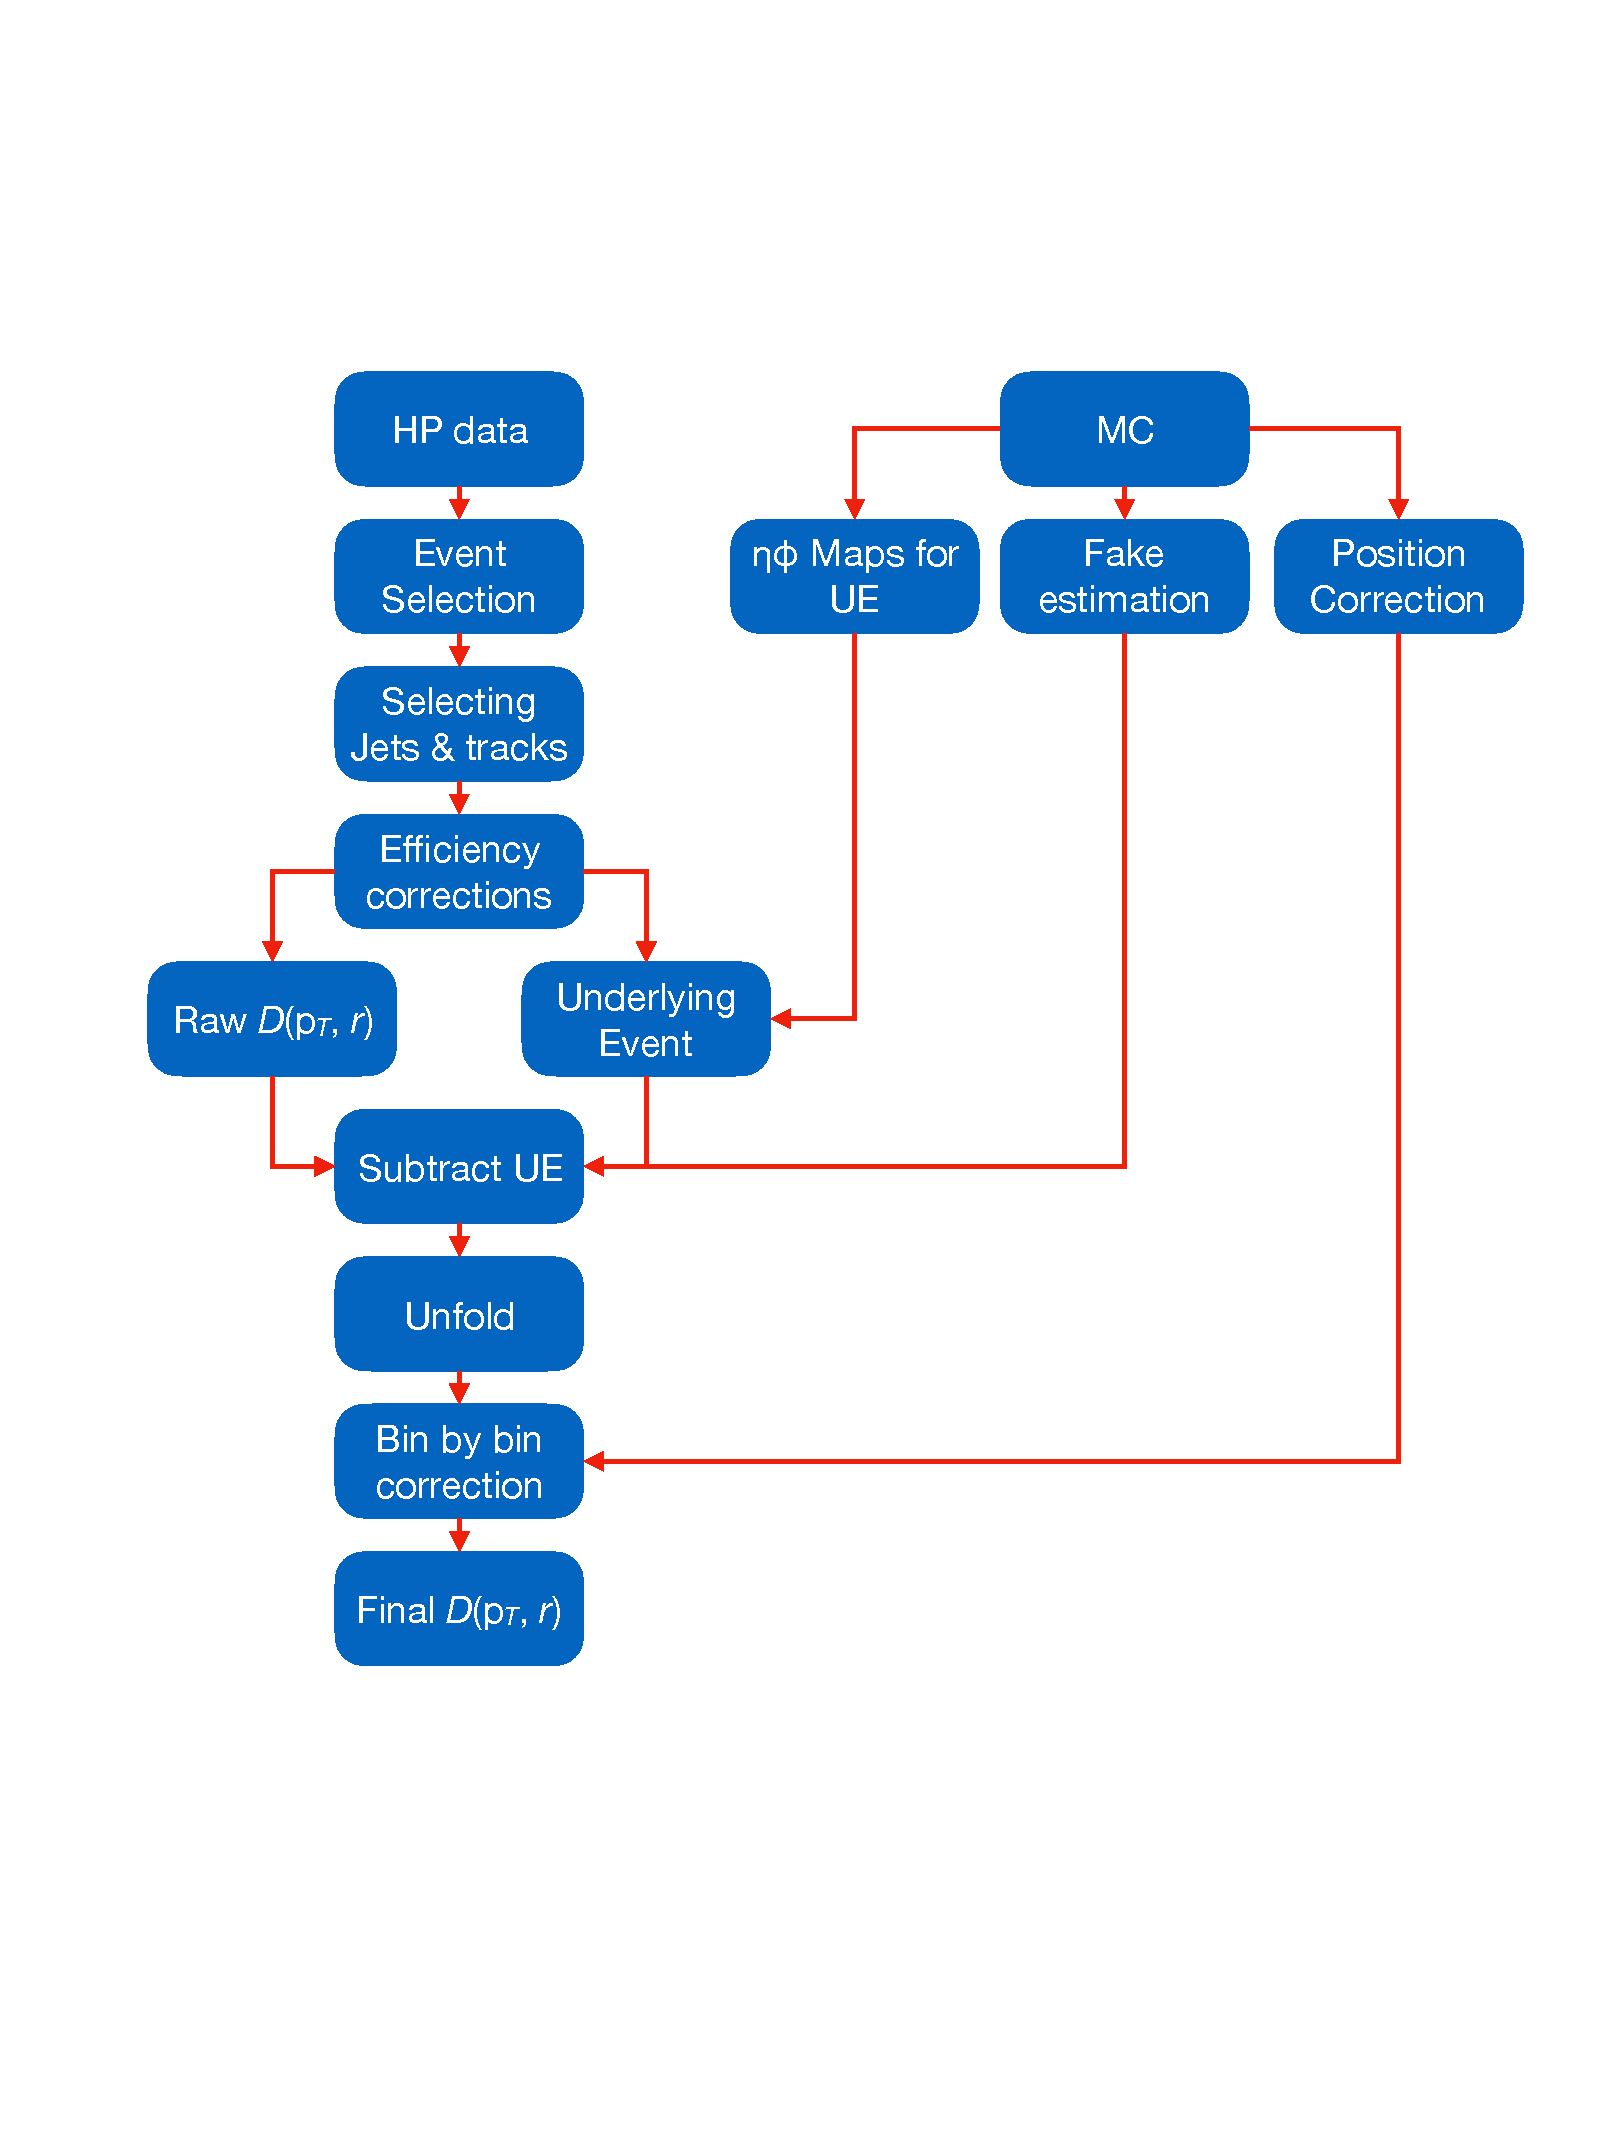
\includegraphics[width=0.6\textwidth]{figures/main/general/Shape_analyses_flow}
\caption{The diagram presents various corrections and cuts that are applied during the analysis.}
\label{fig:analysis_flow}
\end{figure}


\begin{itemize}
\item Jet selection
\item Track selection
\item Track momentum correction
\item Fake rates
\item Tracking efficiency
\item Underlying event subtraction of tracks
\item Unfolding
\end{itemize}




%%%%%%%%%%%%%%%%%%%%%%%%%%%%%%
\subsection{Jet Selection and final energy calibration}
\label{Sec:JetSelection}
Since the Inner Detector (ID) covers the $|\eta| < 2.5$, the analysis can only be performed for jets within the pseudorapidity interval of $|\eta| < 1.7$ to have the entire $ r = $ 0.8 cone under investigation fully covered by the tracking detector.
In both collision systems, jets are measured with \ptjet\ between 126~GeV and 316~GeV in following four successive intervals: 126--158, 158--200, 200--251, and 251--316~GeV.
The \ptjet\ cut is chosen so as to exclude the contribution of ``UE jets'' generated by fluctuations in the underlying event.
This binning is also used in previous heavy ion jet measurements such as Ref.~\cite{PhysRevC.98.024908}.

Truth jets were associated with the nearest reconstructed jet using the matching of $\dR<0.2$ for the performance study and to build response matrices for the unfolding procedure.
The same \dR\ matching criteria were employed in previous ATLAS HI jet analyses and are justified by a detailed performance study~\cite{ATLAS-COM-PHYS-2011-1733}.
To prevent nearby jets from distorting the measurement of \Dptr\ distributions, jets are rejected if there is a neighboring jet with higher \ptjet\ within an angular distance of $\Delta R < 1.0$.
The isolation cut removes approximately 0.01\% of jets (see Figure \ref{fig:ISO}), and has almost no impact on the final measurement.

\begin{figure}
\centering
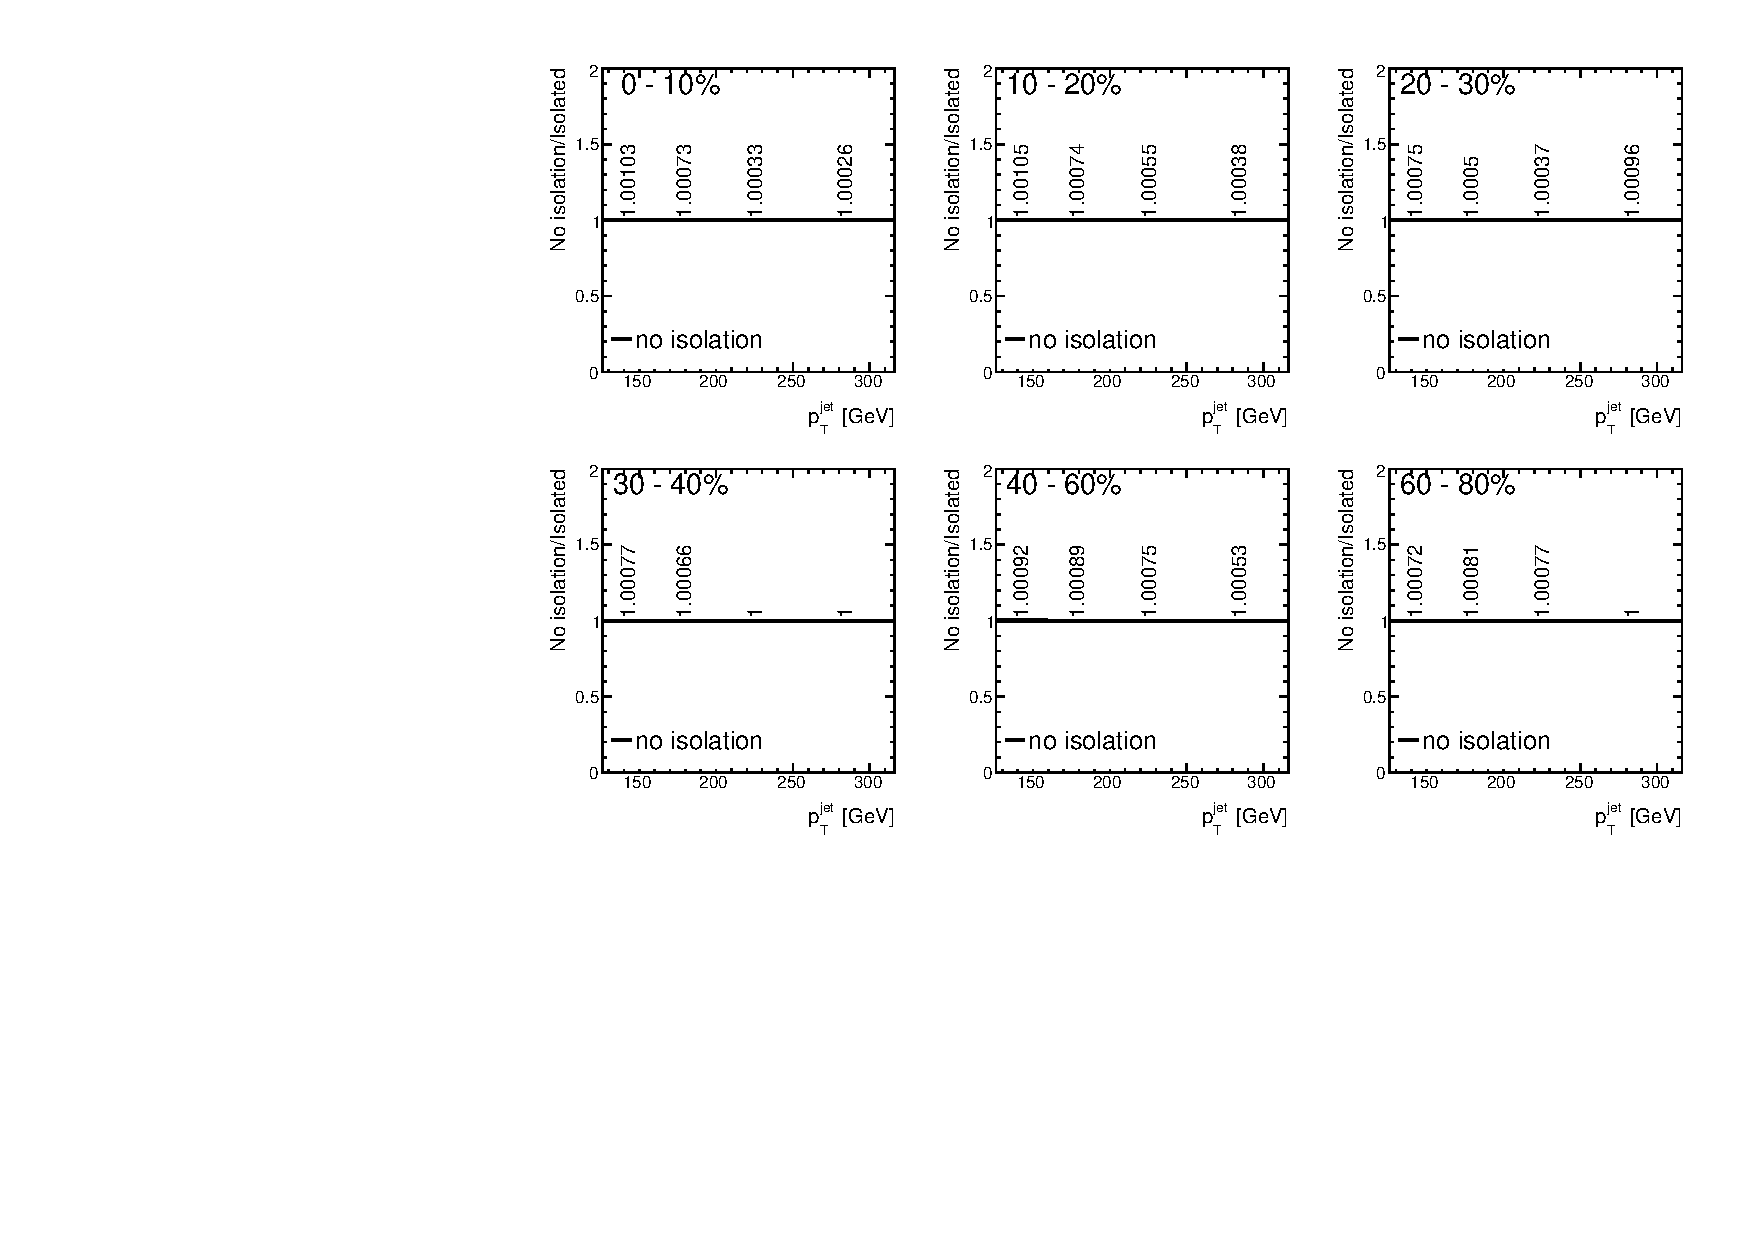
\includegraphics[width=0.70\textwidth]{figures/main/performance/jet_iso.pdf}
\caption{The ratios of the jet spectra with no isolation to that with isolation in the kinematic range of interest for \pbpb\ collisions, in all centralities.
The isolation requirement rejects less that 0.1\% of jets, and has almost no impact on the final measurement.}
\label{fig:ISO}
\end{figure}  

No correction for the jet reconstruction efficiency is necessary, as the analysis is performed in the jet \pT\ region where the jet reconstruction is fully efficient~\cite{2015392}.
The jet energy measured in the calorimeter can be affected by the presence of dead cells or cells with a bad response, by noise spikes in the hadronic end-cap or the EM calorimeter, and by out-of-time energy deposits from cosmic rays and beam backgrounds.
In the \pp\ analysis, these bad jets are removed via a set of standard recommended cuts.
The rate of these jets in the kinematic region of interest (100--316 \GeV) is less than 0.5\%.
This cleaning procedure is not applied in \PbPb\ collisions because it is incompatible with the heavy ion jet reconstruction procedure, and also because the low luminosity ensures noise bursts are negligible.
This is standard procedure for all heavy ion jet analyses.


%%%%%%%%%%%%%%%%%%%%%%%%%%%%%%
\subsection{Track selection}
\label{sec:trackselection}

The track selection cuts used here follow the cuts used in~\cite{PhysRevC.98.024908}.
These provide a low level of fake tracks and a track reconstruction efficiency that is independent of the \pt\ of the jet the track is associated with.

The cuts used here are the ``tight" cuts as described in Ref.~\cite{ref:tracktwiki} and were utilized in previous HI jet fragmentation measurements.
The default tracking cuts used both in \pp\ and \PbPb\ analysis are:
\begin{itemize}
\item{ track $\pT>$~1~GeV}
\item{ track $|\eta|<$~2.5}
\item{ tracks should have at least 9 silicon hits in $|\eta|\leq1.65$}
\item{ tracks should have at least 11 silicon hits in $|\eta|>1.65$}
\item{ tracks should have at least 1 hit in IB-layer + B-layer.}
\item{ tracks should have a IB-layer hit if it is expected, that is, if the track passed an active module.}
\item{ tracks should have a B-layer hit if it is expected and IB-layer hit is not expected.}
\item{ tracks should have  less than 3 holes in silicon detectors.}
\item{ tracks should have 0 holes in pixel detector.}
\item{ impact parameters of track with respect to primary vertex:  $|d_0| < 0.47 e^{(-0.15\pT)} + 0.19 e^{(3.4\rm{E-4}\pT)}$~mm, $|z_0*\sin\theta|<$1.0~mm.
The recommended values are  $|d_0| < 1.5$~mm for tracks with $\pt<10$~GeV and $|d_0| < 0.2$~mm for tracks with $\pt>10$~GeV.
This was chosen to guarantee a smooth behavior of the $d_{0}$ parameter as a function of track momentum.}
\item{All tracks with $\pTch >  \ptjet + \sqrt{ (3 \times \sigma_{\mathrm{JER}}(\ptjet))^2 + (3 \times \sigma_{\mathrm{TMR}}(\pTch))^2} $
%\begin{equation}
%\pTch >  \ptjet + \sqrt{ (3 \times \sigma_{\mathrm{JER}}(\ptjet))^2 + (3 \times \sigma_{\mathrm{TMR}}(\pTch))^2} 
%\end{equation}
are rejected from the analysis, where the TMR stands for track momentum resolution.
The purpose of this cut is to be consistent with previous fragmentation measurements~\cite{PhysRevC.98.024908}.
It has minimal impact on this analysis because the analysis is restricted to tracks below 63 GeV and jets above 100 GeV.}
\end{itemize}


A tighter tracking selection is used for systematic studies (``tight+'' cuts).
These cuts include all of the default cuts plus a 3$\sigma$ cut on the significance of the $d_0$ and $z_0 \sin\theta$.
Figures~\ref{fig:trkdataMCcomp_pp}-\ref{fig:trkdataMCcomp_pbpb_highpt} shows comparisons of the data and MC tracking quantities in \pp\ and \pbpb\ collisions, respectively, for different track \pT\ intervals.
It can be seen that the MC describes the data well.
A 20\% discrepancy is observed for low impact parameters.
The discrepancy is present far from the values of corresponding tracking cuts.
There is a small shift in the $z0$ distribution in the MC samples.
This difference is caused by the allowance of a small difference in the $z$ position of the primary vertex in the MC overlay procedure.
However this has negligible impact on the analysis as the overall quality requirement on the pointing parameter in the $z0$ is 1~mm.
Furthermore, Figure~\ref{fig:trkdataMCcomp_pbpb_highpt} shows the same comparison for high \pt\ tracks.
All the comparisons of distributions show the same qualitative features as seen at lower \pt\ with improving pointing with increasing track \pt.
The comparison of the reconstructed \pttrk\ with the generated kinematics for tracks passing these cuts is shown in Figure~\ref{fig:momres_pp}.

\begin{figure}
\centering{
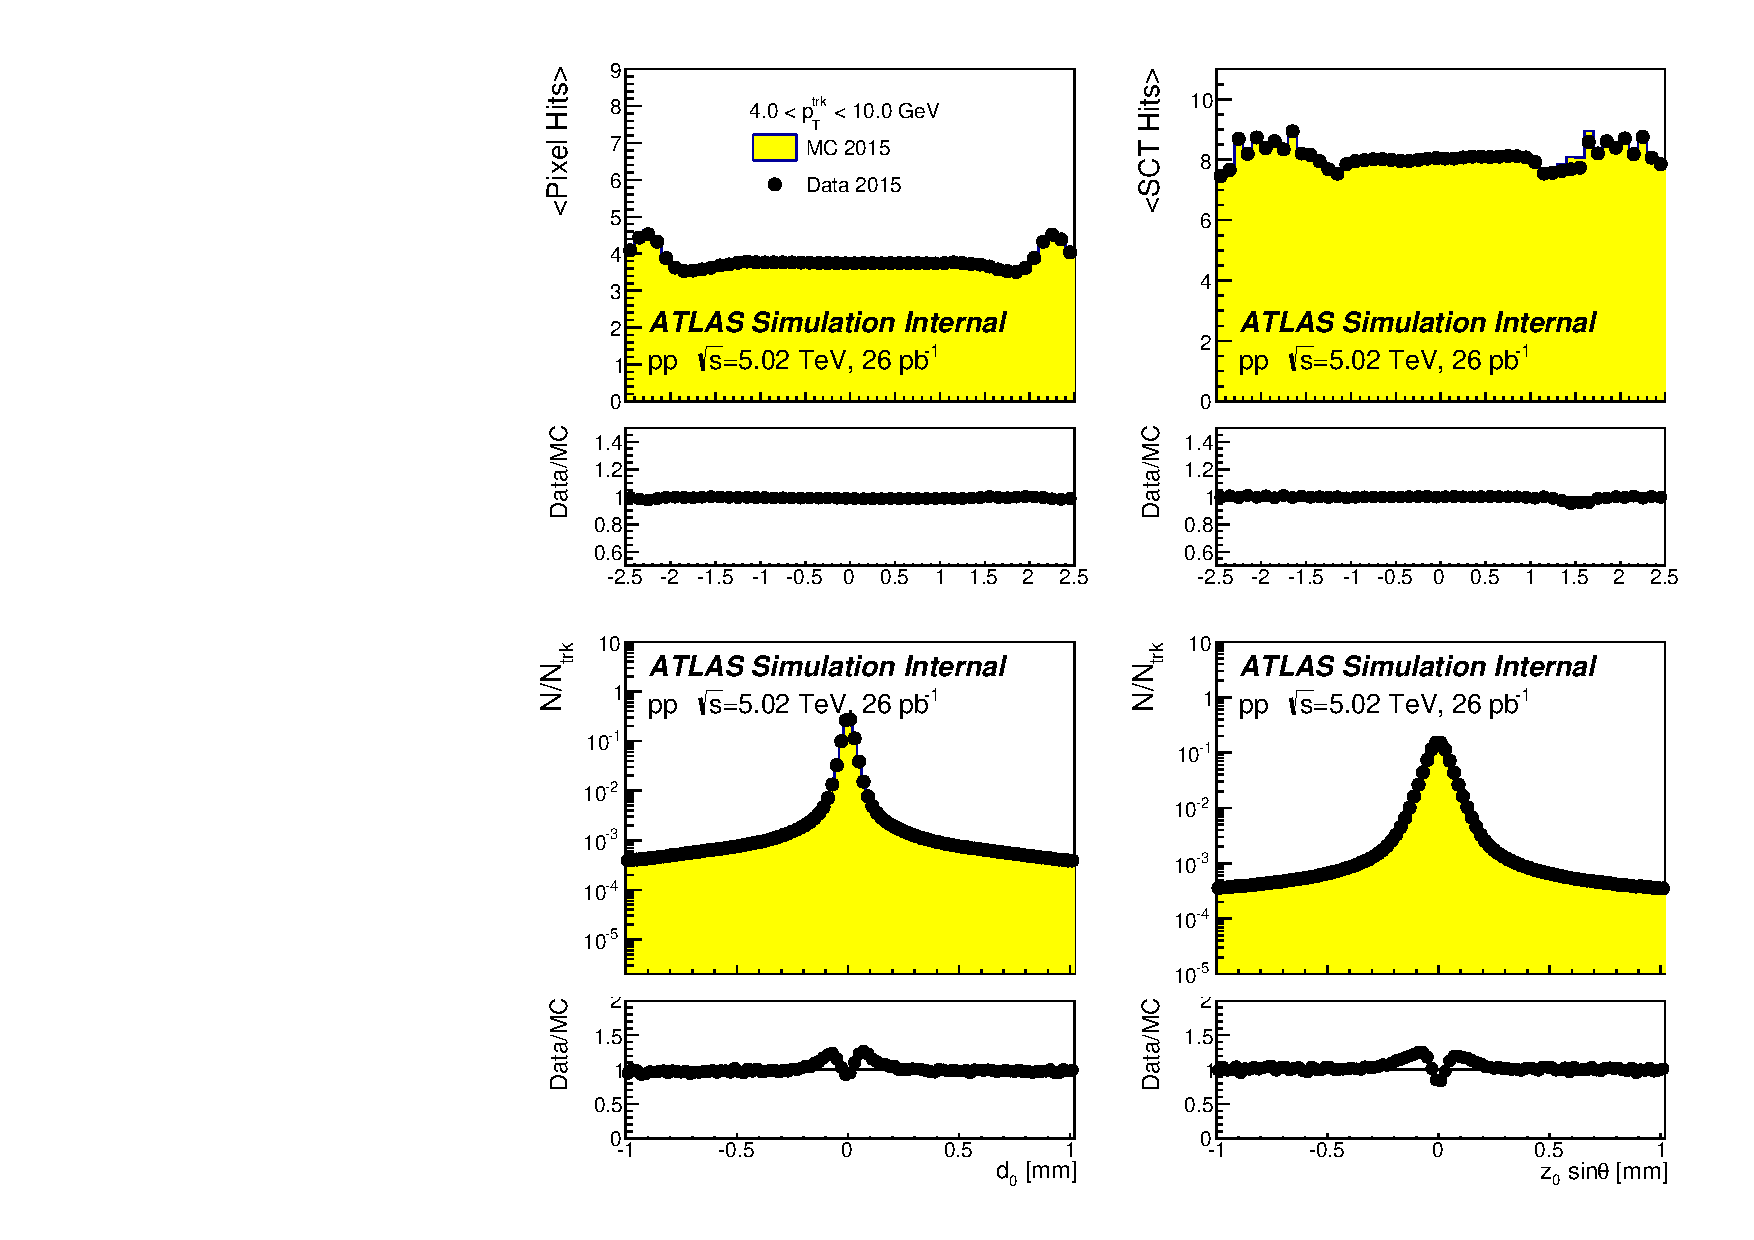
\includegraphics[width=0.75\textwidth]{figures/main/performance/TrkPerforPlots_5TeV_pp.pdf} }
\caption{Track quantity comparison between data (points) and MC (yellow histogram) in \pp\ collisions.
Tracks are selected to have 4.2~$<\pttrk<$~10~GeV.
Below each direct data and MC overlay is the corresponding data to MC ratio.
The quantities compared are: average number of pixel hits as a function of $\etatrk$ (top left), average number of SCT hits as a function of $\etatrk$ (top right), and number of tracks, $N_{\mathrm{trk}}$, normalized $d_0$ (bottom left), and $z_0 \sin\theta$ distributions (bottom right).
Figure from Ref.~\cite{Sickles:2235420}.}
\label{fig:trkdataMCcomp_pp}
\end{figure}

\begin{figure}
\centering{
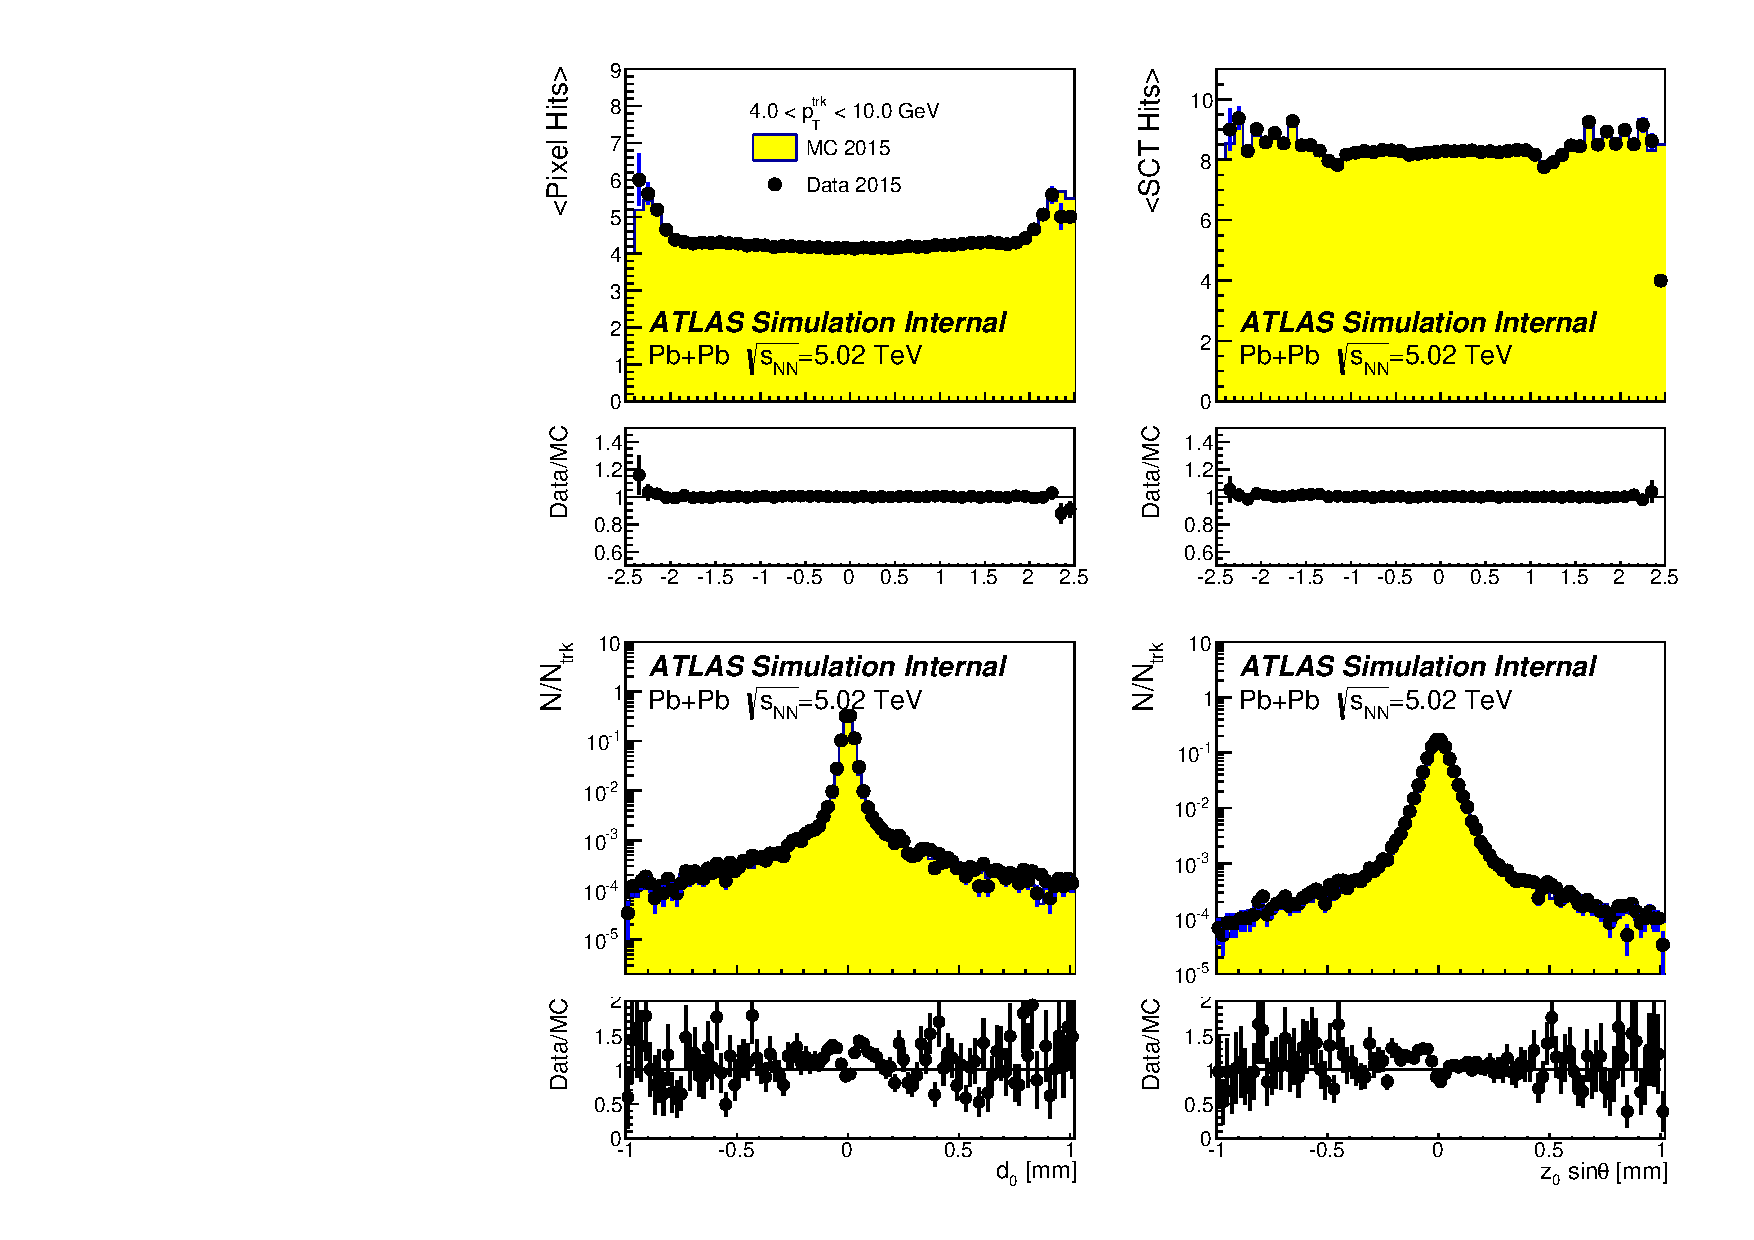
\includegraphics[width=0.75\textwidth]{figures/main/performance/TrkPerforPlots_PbPb_pt4p2_10p0GeV.pdf} }
\caption{Track quantity comparison between data (points) and MC (yellow histogram) in 0-10\% central \pbpb\ collisions.
Tracks are selected to have 4.2~$<\pttrk<$~10~GeV.
Below each direct data and MC overlay is the corresponding data to MC ratio.
The quantities compared are: average number of pixel hits as a function of $\etatrk$ (top left), average number of SCT hits as a function of $\etatrk$ (top right), track $d_0$ (bottom left), and track $z_0 \sin\theta$ (bottom right).
Figure from Ref.~\cite{Sickles:2235420}.}
\label{fig:trkdataMCcomp_pbpb}
\end{figure}

\begin{figure}
\centering{
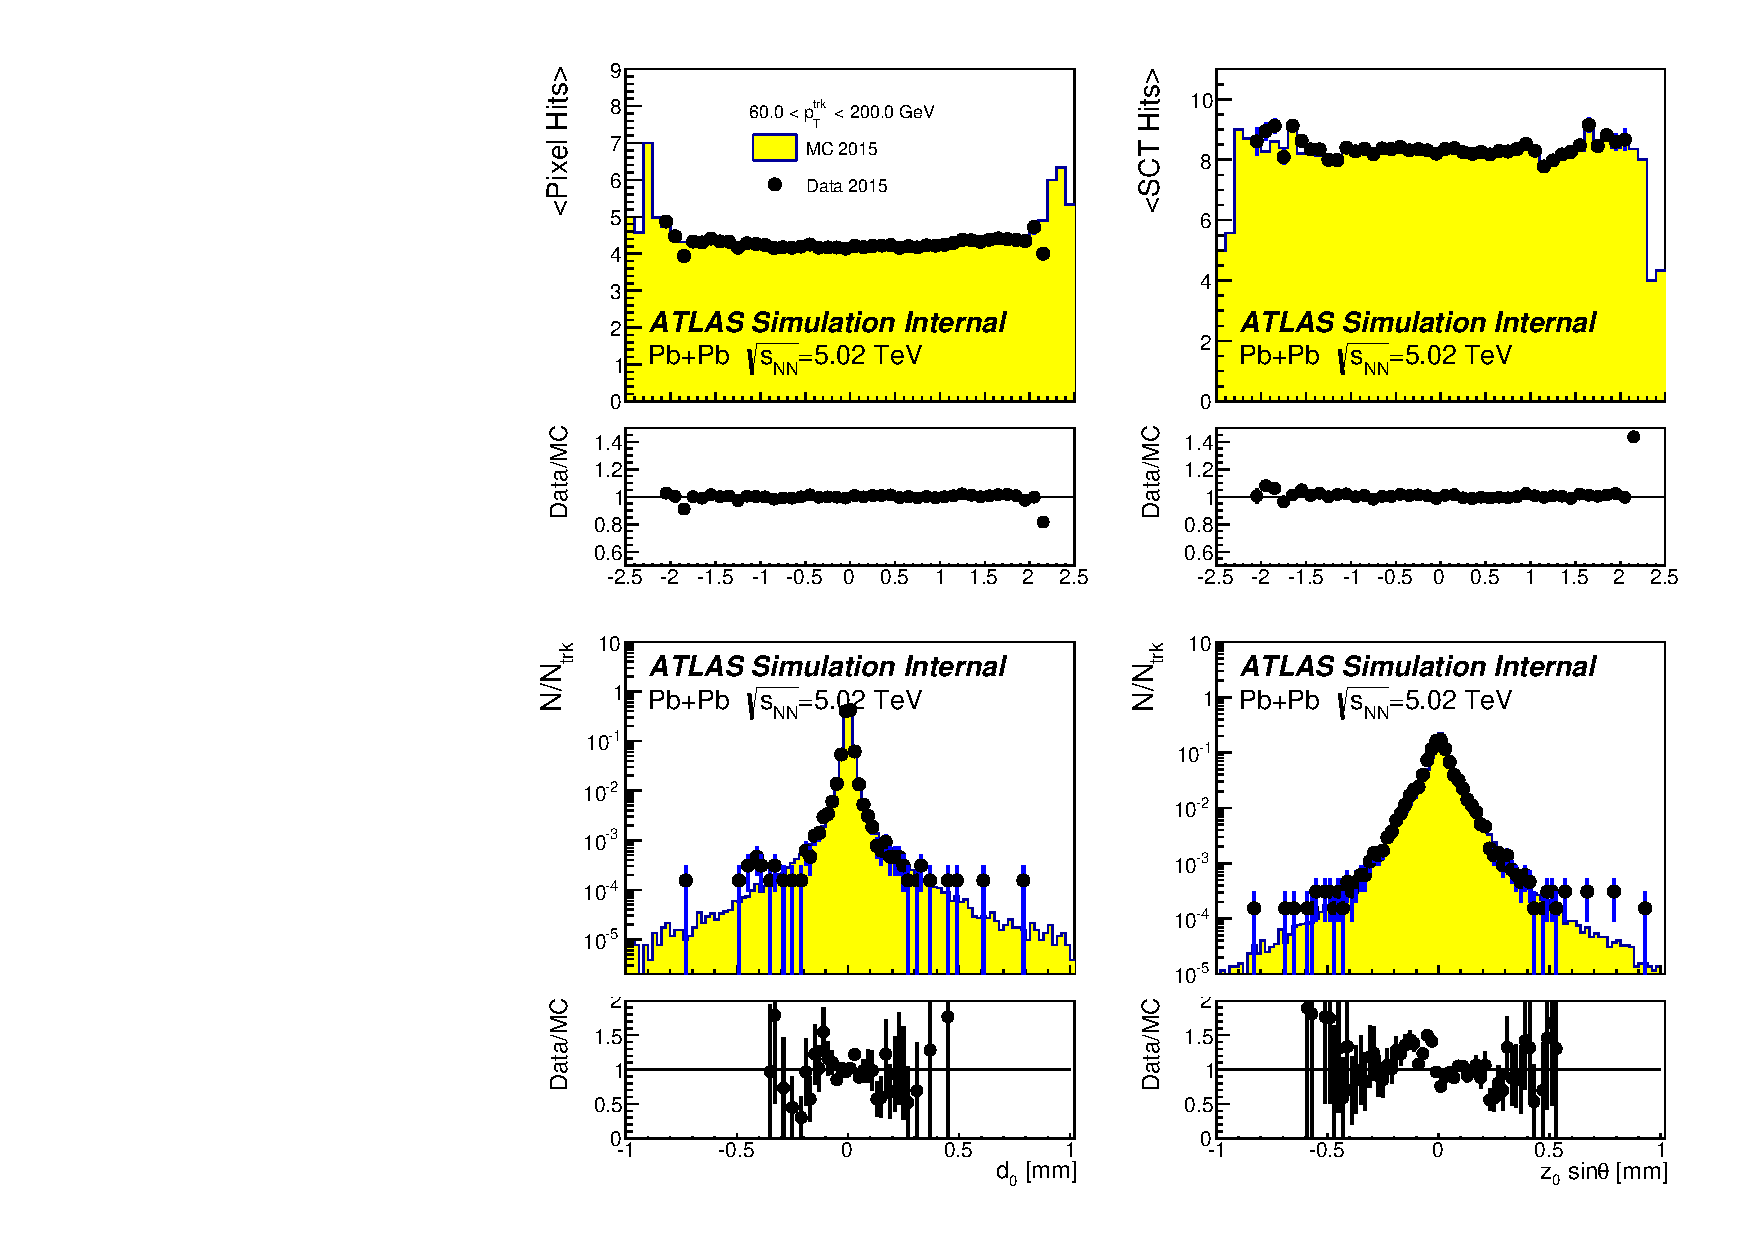
\includegraphics[width=0.75\textwidth]{figures/main/performance/TrkPerforPlots_PbPb_pt60_200GeV.pdf} }
\caption{Track quantity comparison between data (points) and MC (yellow histogram) in \pbpb\ collisions inclusive in collisions centrality.
Tracks are selected to have 60~$<\pttrk<$~200~GeV and to originate from jet with \pt\ in the interval from 251 to 316 GeV.
Below each direct data and MC overlay is the corresponding data to MC ratio.
The quantities compared are: average number of pixel hits as a function of $\etatrk$ (top left), average number of SCT hits as a function of $\etatrk$ (top right), track $d_0$ (bottom left), and track $z_0 \sin\theta$ (bottom right).
Figure from Ref.~\cite{Sickles:2235420}.}
\label{fig:trkdataMCcomp_pbpb_highpt}
\end{figure}


\begin{figure}
\centering{
\begin{tabular}{cc}
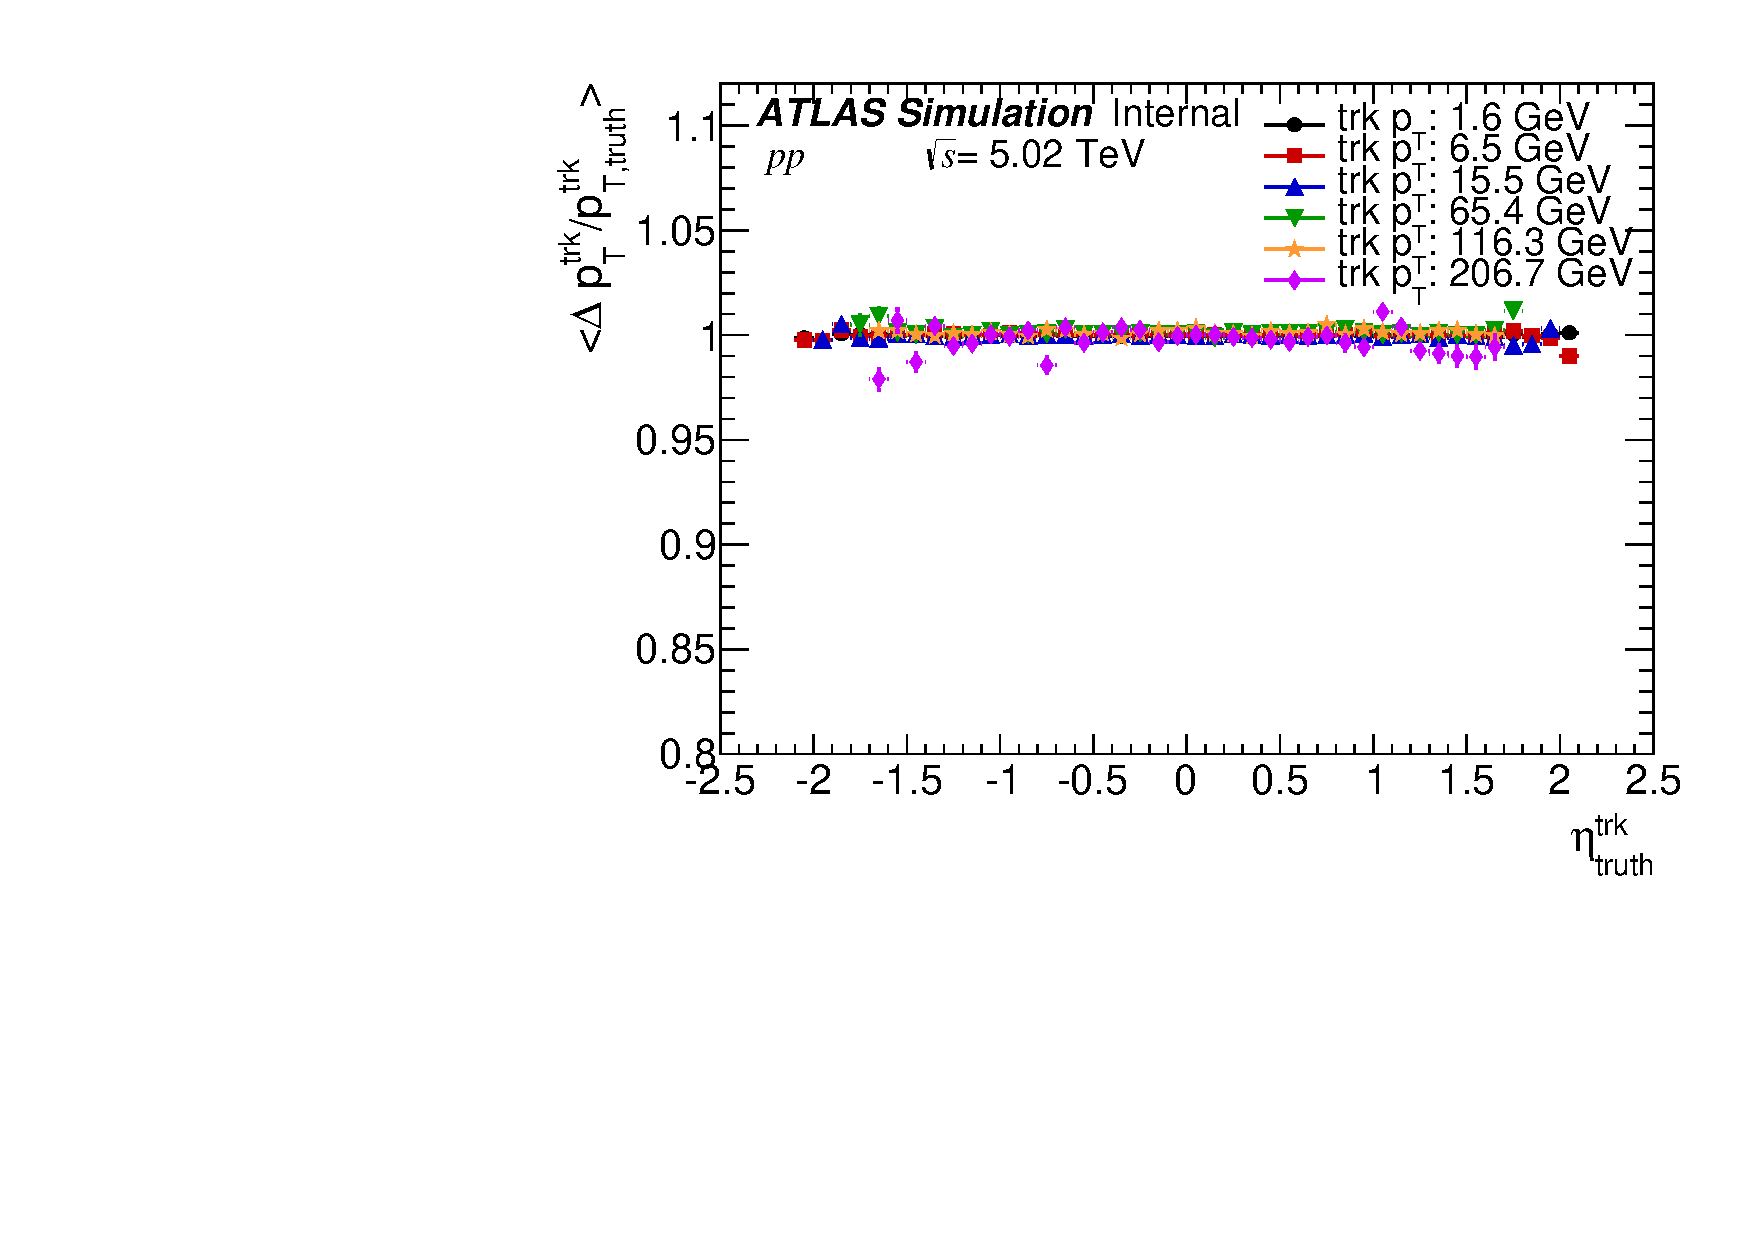
\includegraphics[width=0.45\textwidth]{figures/main/performance/scale_v_eta_pp.pdf} &
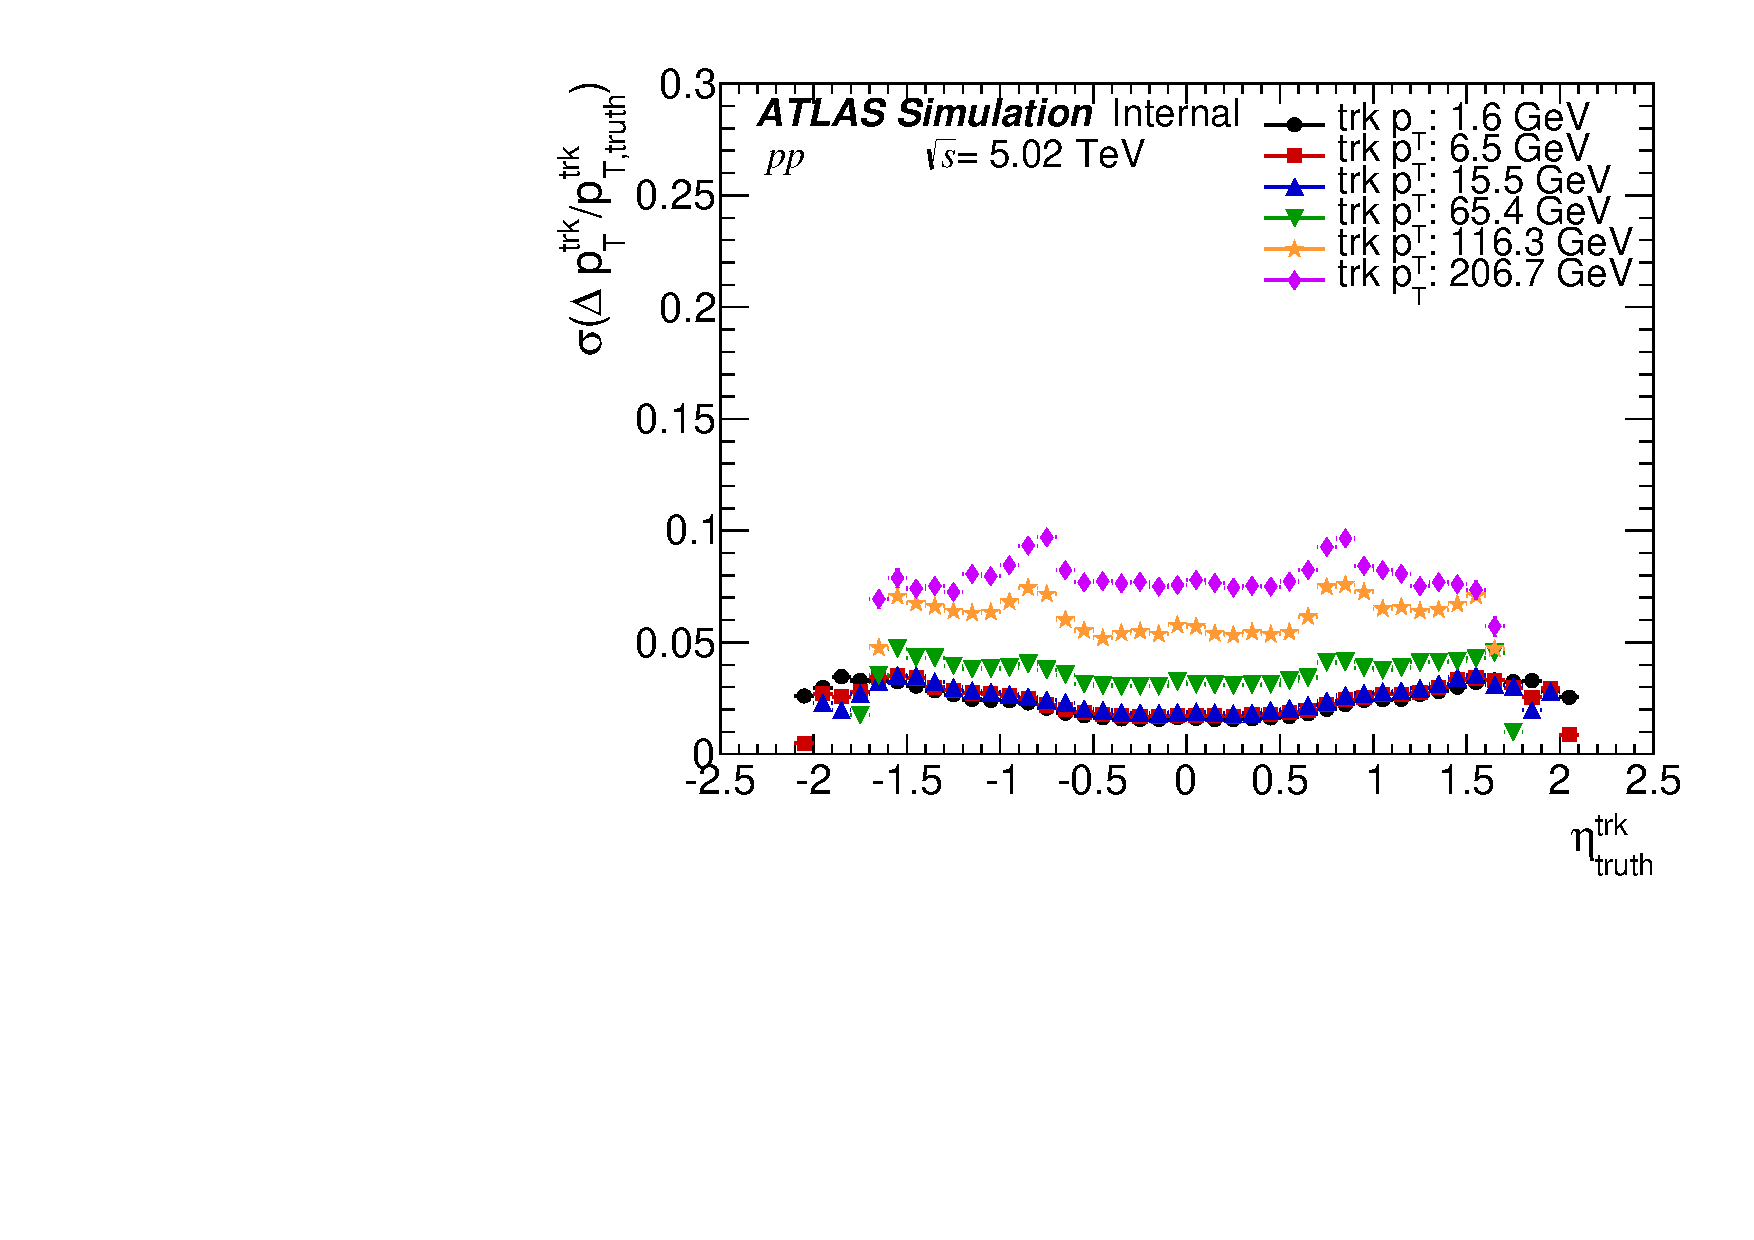
\includegraphics[width=0.45\textwidth]{figures/main/performance/resolution_v_eta_pp.pdf} \\ 
\end{tabular}}
\caption{(left) Comparison of the generated and reconstructed track \pt\ as a function of \etatrktruth\ for five track \pttrktruth\ selections.
(right) Track momentum resolution as a function of \etatrktruth\ for five \pttrktruth\ selections.
Both plots are for \pp\ MC.
All tracks shown in this plot have passed the 2015 default tracking cuts defined in this section.
The \pt\ in the legend corresponds to the bin centers in the following track \pt\ bins: 1.3 -- 1.8 GeV, 5.6 -- 7.5 GeV, 13.3 -- 17.7 GeV, 56.1 -- 74.8 GeV, 99.7 -- 132.9 GeV, \mbox{177.2 -- 236.2 GeV}.
Figure from Ref.~\cite{Sickles:2235420}.}
\label{fig:momres_pp}
\end{figure}



Figure~\ref{fig:ppcutflow_eta} presents the impact of individual tracking requirements in terms of the ratio of the number of tracks that pass given cut and the total number of reconstructed tracks in \pp\ MC.
This is shown as a function of track pseudorapidity in two different track \pT\ intervals and as a function of track \pT\ in two different pseudorapidity intervals.
The highest rejection for low \pT\ tracks is provided by the cut on $d_{0}$ pointing.
At high \pT\, the dominant effect is seen from the requirement on the number of silicon hits.
Similarly, Figure~\ref{fig:PbPbcutflow_eta} presents the impact of individual tracking requirements in \PbPb\ MC.
The difference between the impact of individual cuts can be attributed to a different setting of the tracking algorithm and to the overall increase of the track multiplicity as the number of rejected tracks does not linearly scale with the multiplicity that enters the denominator.


The primary particles\footnote{Primary particles are defined as particles with a mean lifetime $\tau>0.3\times 10^{-10}$ s either directly produced in \pp\ interactions or from subsequent decays of particles with a shorter lifetime.All other particles are considered to be secondary.}
used in this analysis have a mean lifetime \mbox{$\tau > 0.3 \times 10^{-10}$~s} and are either directly produced in \pp\ interactions or from subsequent decays of particles with a shorter lifetime.
They are required to have their barcode in the range $0 - 200000$.
Of these, particles with barcode $< 10000$ are coming from Pythia, while the remaining are from HIJING.
Particles with barcodes above 200000 are secondaries, and come from weak decays of $\Lambda$, $K_{S}$, $\Xi$, $\Sigma$, $\Omega$ and from particles created in interactions with the material.
Strange baryons are included: $\Sigma-$ (PDG ID 3112), $\Sigma+$ (PDG ID 3222), $\Xi-$ (PDG ID 3312), $\Omega-$ (PDG ID 3334).


\begin{figure}
\centering
\begin{tabular}{cc}
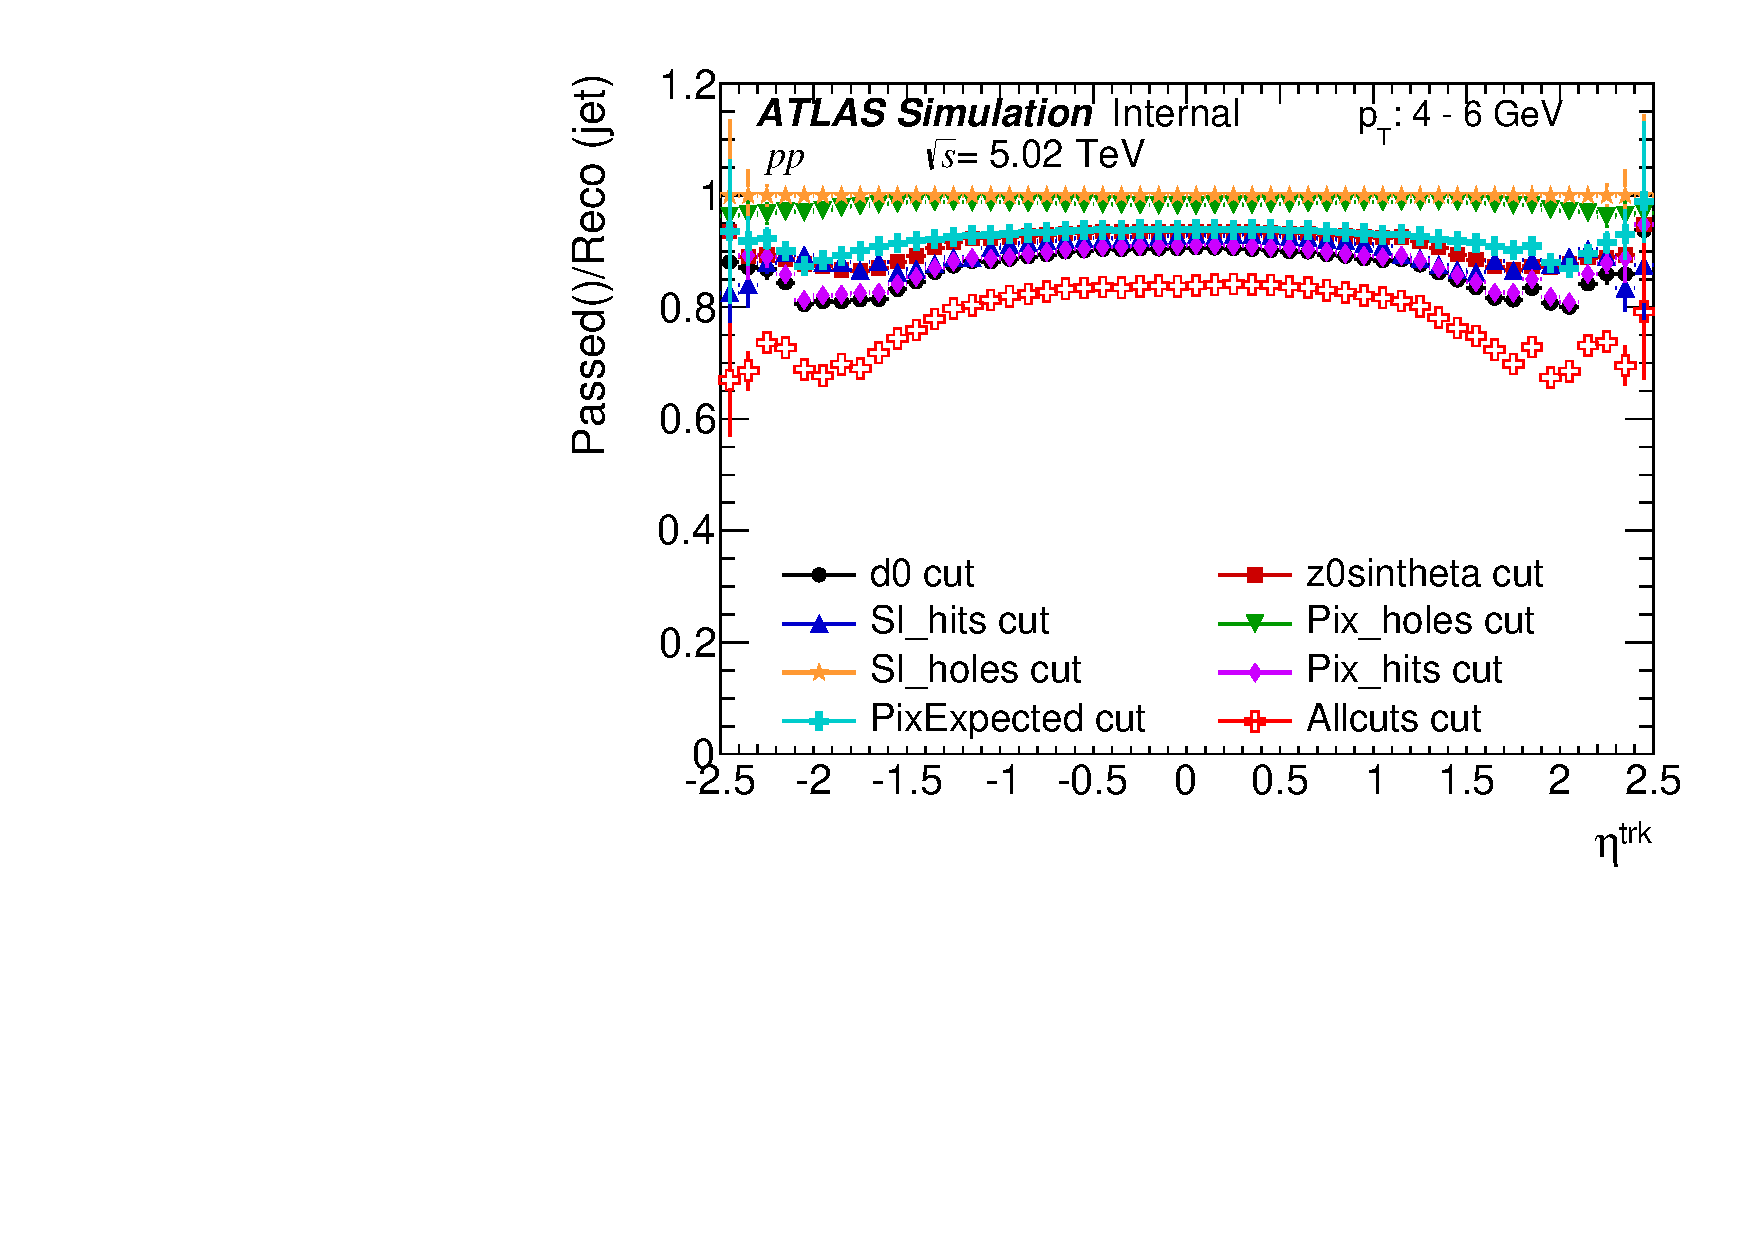
\includegraphics[width=0.45\textwidth]{figures/main/performance/cut_flow_RecoNorm_MC_pT_4_6_jet.pdf} &
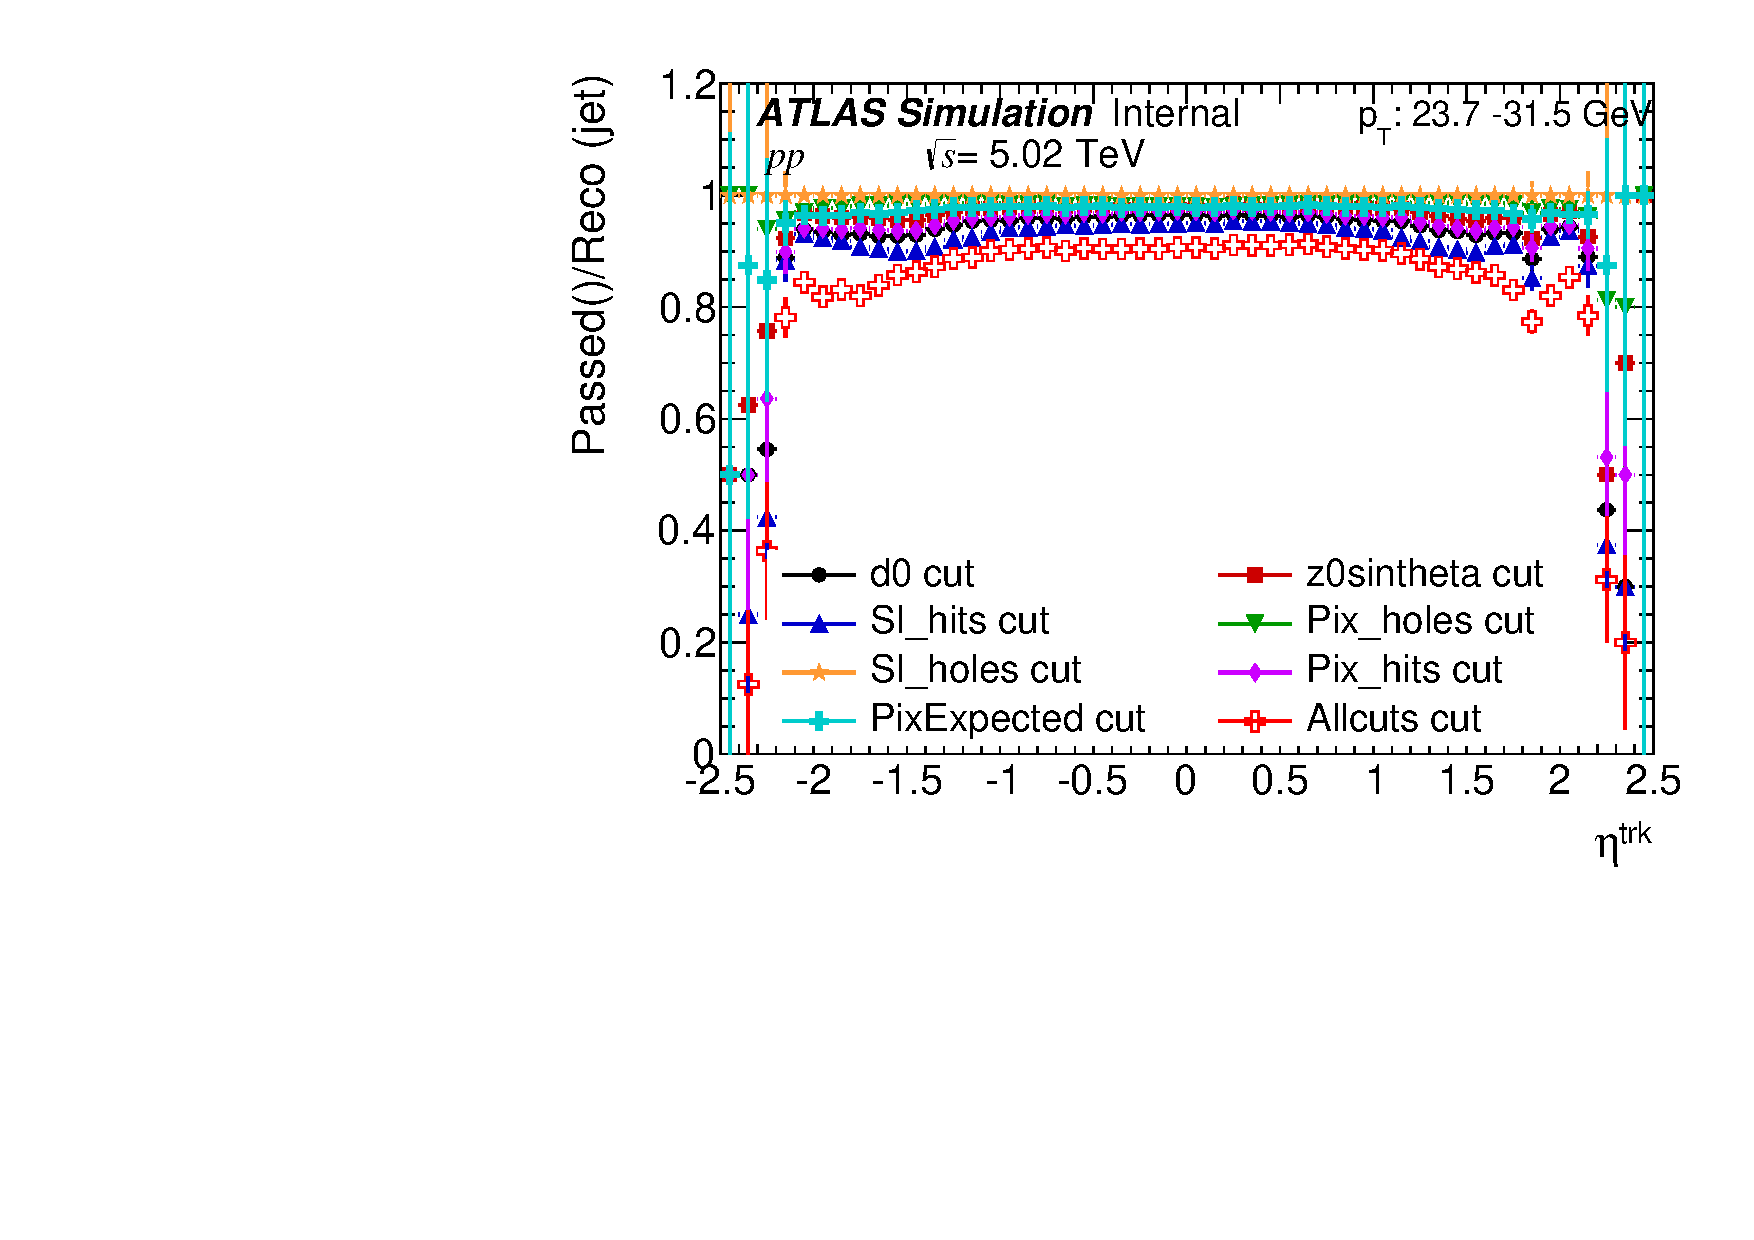
\includegraphics[width=0.45\textwidth]{figures/main/performance/cut_flow_RecoNorm_MC_pT_23p7_31p5_jet.pdf} \\
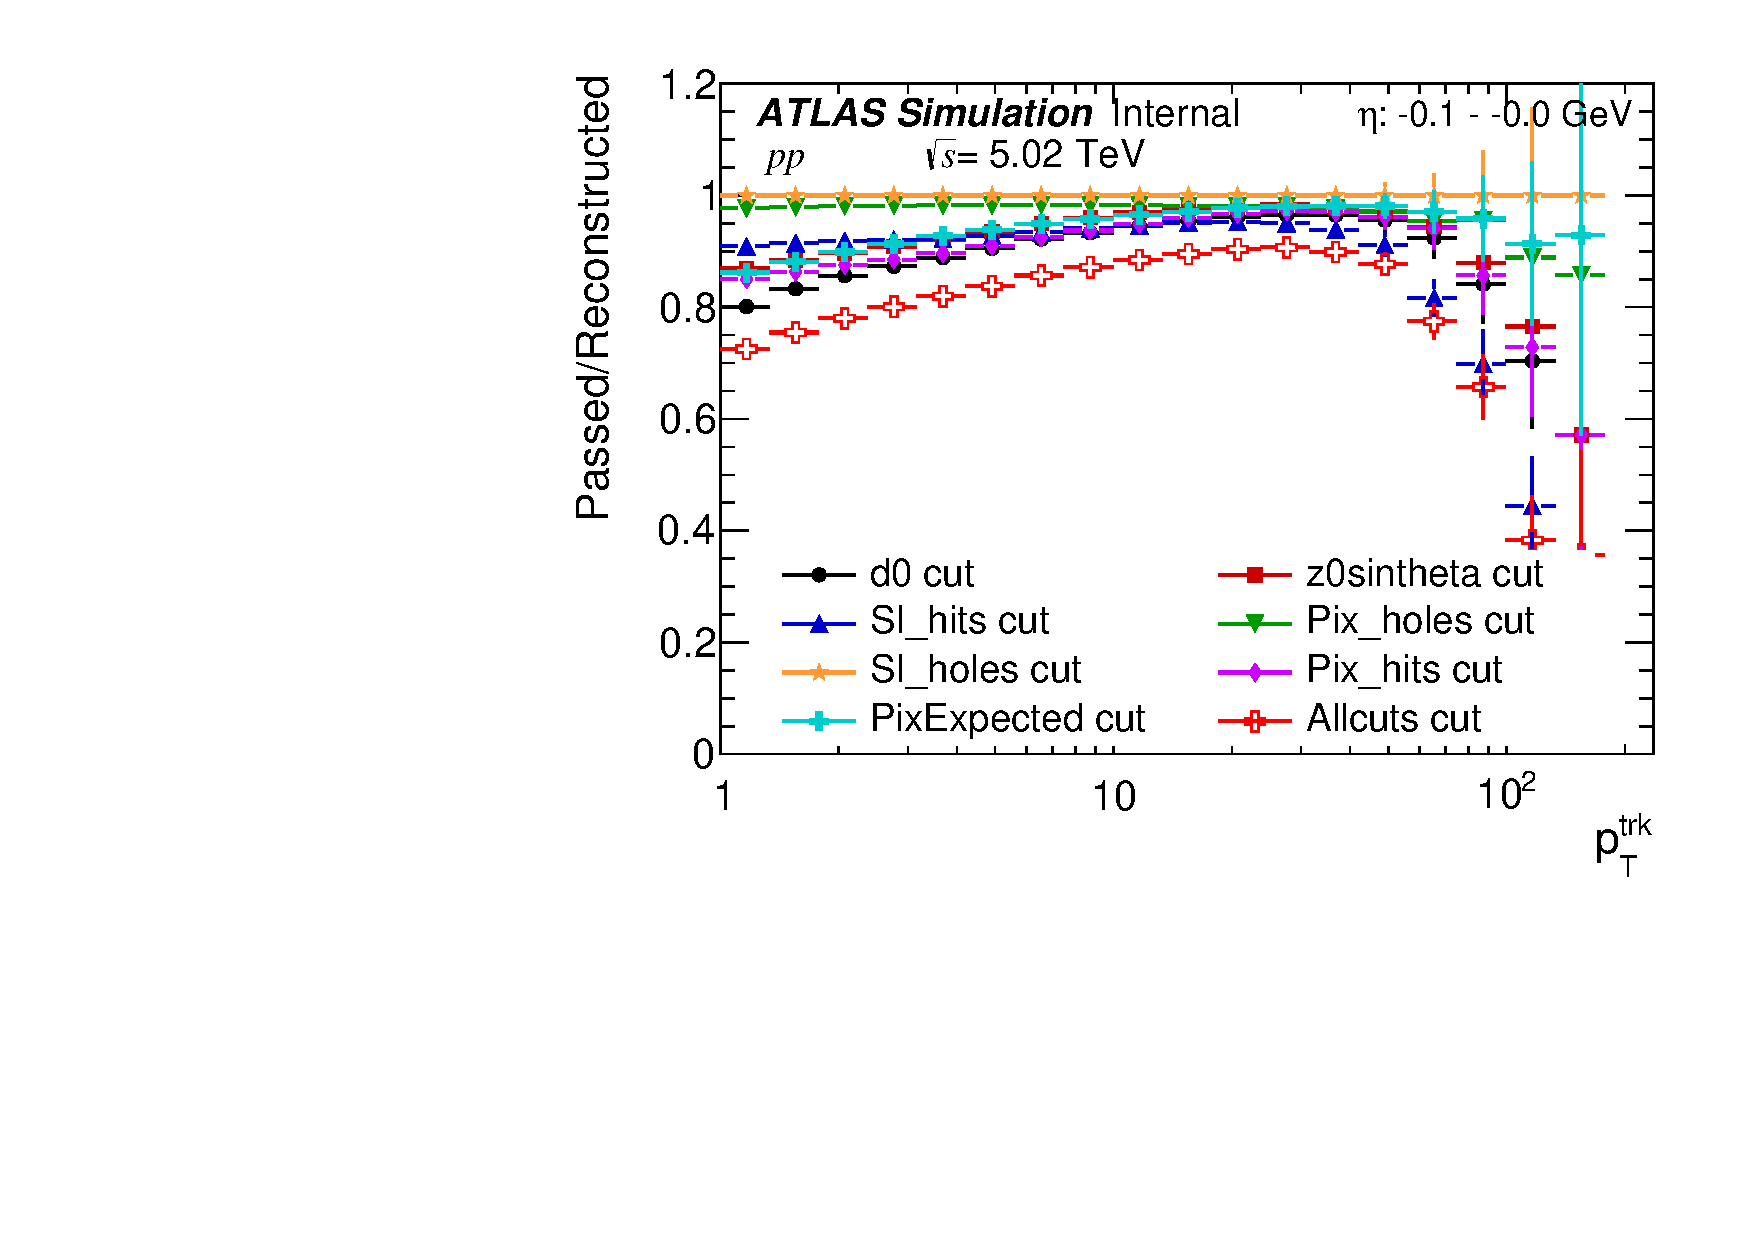
\includegraphics[width=0.45\textwidth]{figures/main/performance/cut_flow_RecoNorm_MC_eta_0p05_jet.pdf} &
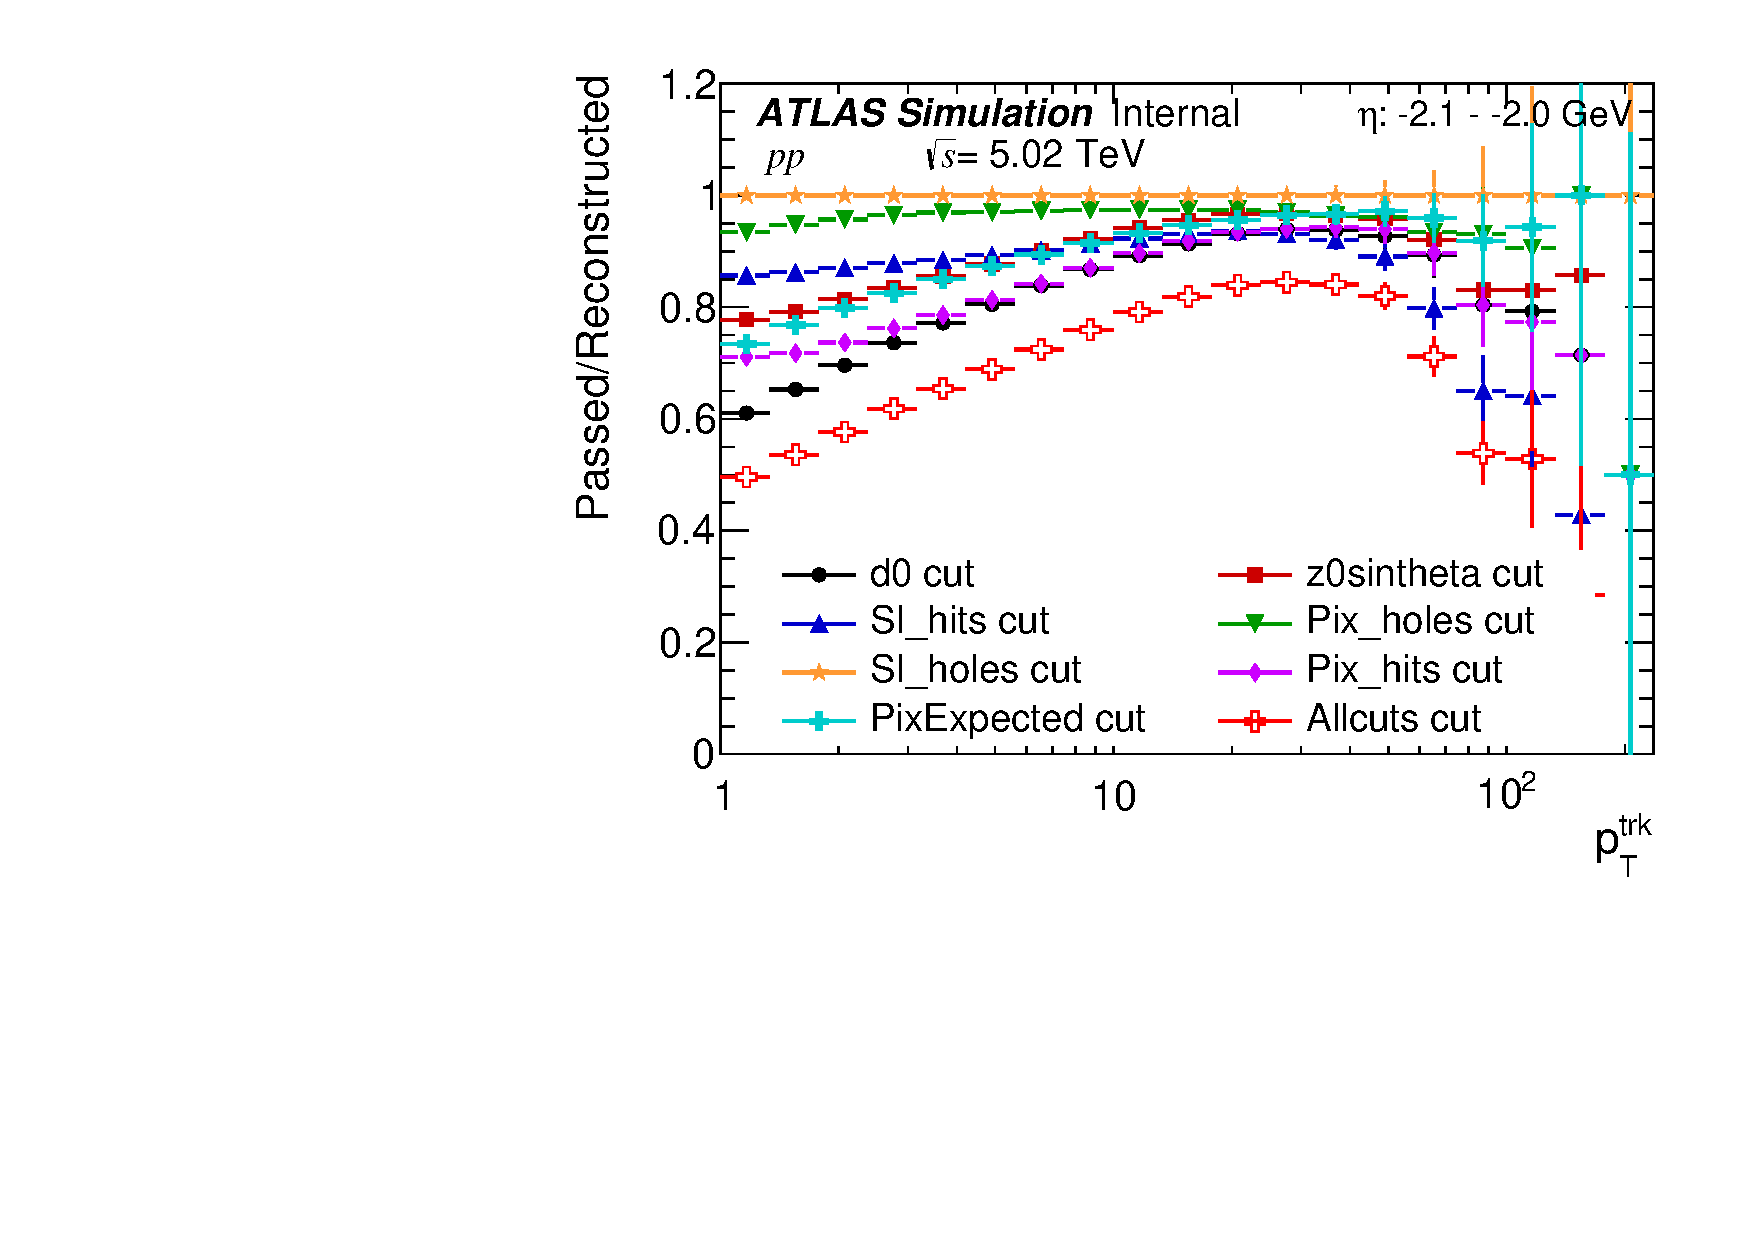
\includegraphics[width=0.45\textwidth]{figures/main/performance/cut_flow_RecoNorm_MC_eta_2p05_jet.pdf} \\
\end{tabular}
\caption{The impact of each cut applied individually in the \pp\ MC to the starting collection of tracks, as a function of
\etatrk (top) for 1.3~$< \pttrk<$~4.6~GeV (left) and for 23.7~$<\pttrk<$~31.5~GeV and as a function of track \pT\ for two different pseudorapidity intervals (bottom).
The final combination of all cuts is shown as well.
Figure from Ref.~\cite{Sickles:2235420}.}
\label{fig:ppcutflow_eta}
\end{figure}

\begin{figure}
\centering
\begin{tabular}{cc}
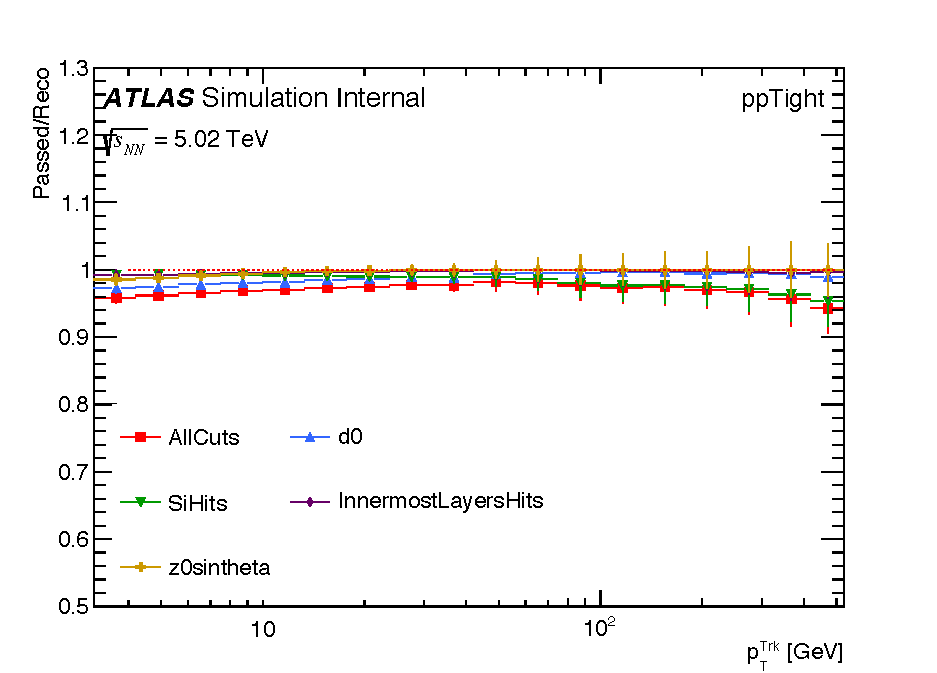
\includegraphics[width=0.45\textwidth]{figures/main/performance/PbPb_cutflow_pptight.pdf} &
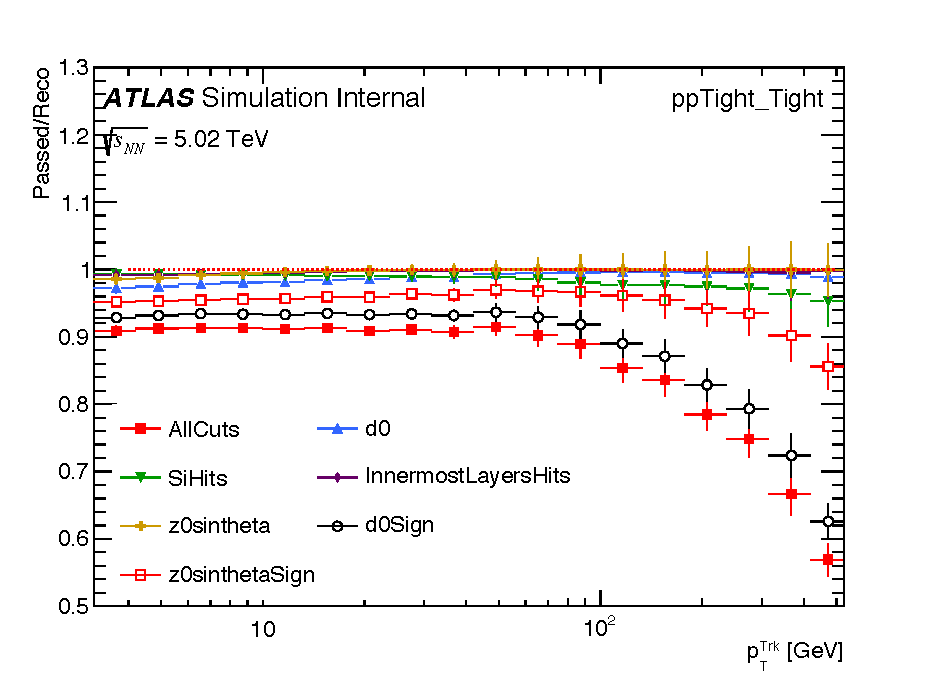
\includegraphics[width=0.45\textwidth]{figures/main/performance/PbPb_cutflow_pptight_tight.pdf} \\
\end{tabular}
\caption{The impact of each cut applied individually in the \PbPb\ MC 
to the starting collection of tracks, as a function of the track \pT\ inclusive in collision centrality for the default and the tight set of tracking requirements.
The final combination of all cuts
is shown as well.}
\label{fig:PbPbcutflow_eta}
\end{figure}



%%%%%%%%%%%%%%%%%%%%%%%%%%%%%%
\subsection{Track momentum correction}
\label{Sec:Trackmomentumcorrection}
Specific corrections are needed for track momentum in 5.02~TeV \pp\ and \PbPb\ data to account for a miss-alignment introduced in the track reconstruction.
The sign charge dependent momentum scale shift was observed in \pp\ data when the transverse momentum of muons reconstructed using muon spectrometer was compared to the transverse momentum of muons from the inner detector.
The difference as a function of muon momentum in \pbpb\ data can be seen in Figure~\ref{fig:ChMomentumScale}.
The correction to track \pt\ as a function of track $\eta$ and track $\phi$ is applied through sagitta bias maps introduced in Ref.~\cite{TrackingRec}.

\begin{figure}[h]
\centering
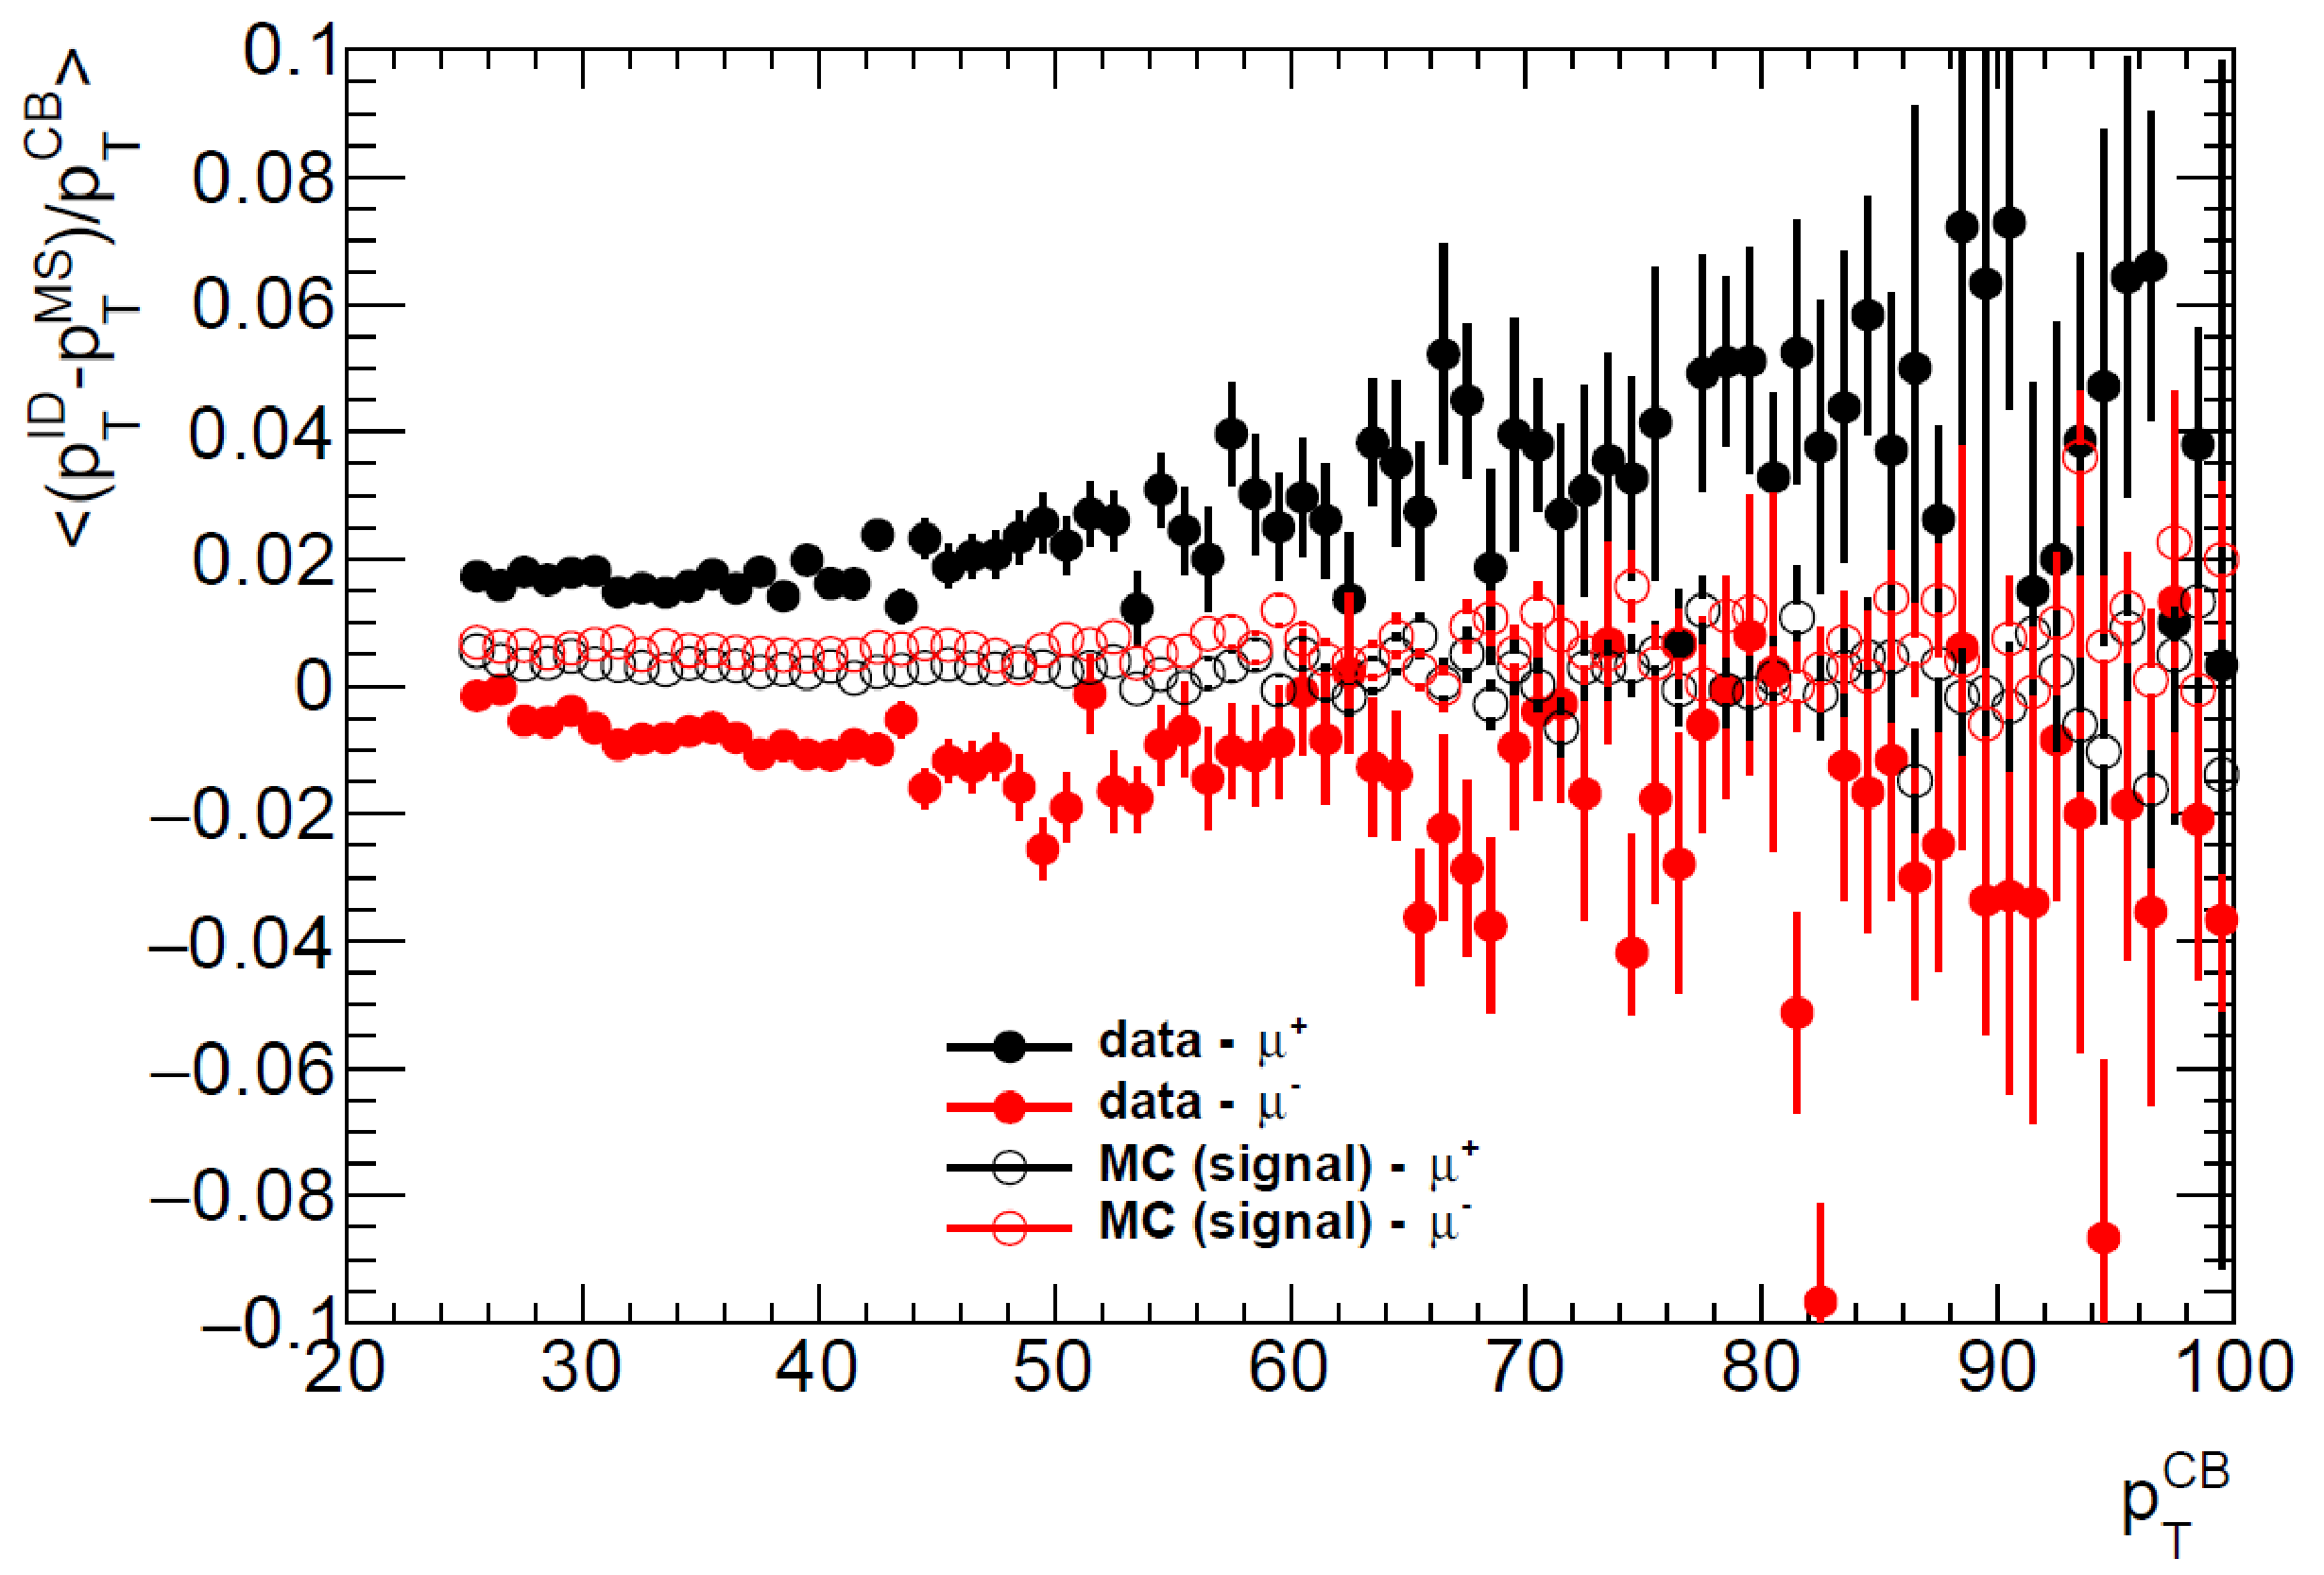
\includegraphics[width=0.55\textwidth]{figures/main/corrections/MuonPerf.pdf}
\caption{Comparisons of track momentum scale of positive and negative muons reconstructed using muon spectrometer and inner detector.
The muon traverse momentum evaluated from muon spectrometer (MC) is compared by that evaluated using the inner detector (ID) and the relative scale is normalized by the momentum that uses both detectors.
Figure from Ref.~\cite{Bold:2194917}.}
\label{fig:ChMomentumScale}
\end{figure}


%%%%%%%%%%%%%%%%%%%%%%%%%%%%%%
\subsection{Track reconstruction efficiency}
\label{sec:trackreco}

The tracking reconstruction efficiency is defined as the ratio between the number of primary truth charged particles that are reconstructed and the total number of primary truth charged particles in the given \pt\ and $\eta$ bin.
It is evaluated using MC tracks, where tracks are required to pass all the tracking cuts imposed on the data.

Matching between the reconstructed and the truth track is done via a cut on \mcprob.
This is defined as the probability that a reconstructed track matched to a truth track actually was a truth track.
It is calculated as:

\begin{align}
\mcprob = \frac{10N^{\mathrm{common}}_{\mathrm{pix}} + 5N^{\mathrm{common}}_{\mathrm{SCT}} + N^{\mathrm{common}}_{\mathrm{TRT}}}{10N^{\mathrm{track}}_{\mathrm{pix}} + 5 N^{\mathrm{track}}_{\mathrm{SCT}} + N^{\mathrm{track}}_{\mathrm{TRT}}}
\end{align}
where $N^{\mathrm{common}}_X$  are the number of hits in detector $X$ in common between the truth and reconstructed track.
$N^{\mathrm{track}}_X$ is the number of total hits in the reconstructed track.

Tracks with $\mcprob > 0.3$ are associated with the truth track and those with a lower value are not and are classified as fake tracks.
The choice of $\mcprob = 0.3$ is based on the recommendation from the ATLAS tracking group and was used in~\cite{201865}.
The sensitivity of the measurement on the value of the \mcprob\ cut is included in the systematic uncertainties.

In MC samples, the ``track barcode'' classifies reconstructed tracks to different classes based on the origin (primary, secondary, pileup, beam halo, fake).
We require $0 < \mathrm{barcode} < 200000$ in evaluation of the tracking efficiency to remove pileup, beam halo, secondary particles, and fake particles.
Reconstructed tracks that do not have a matched truth track with given \mcprob\ are labeled all together as fake tracks.
The tracking cuts need to provide both good efficiency for generator level tracks and to adequately reject fakes.

\begin{figure}
\centering
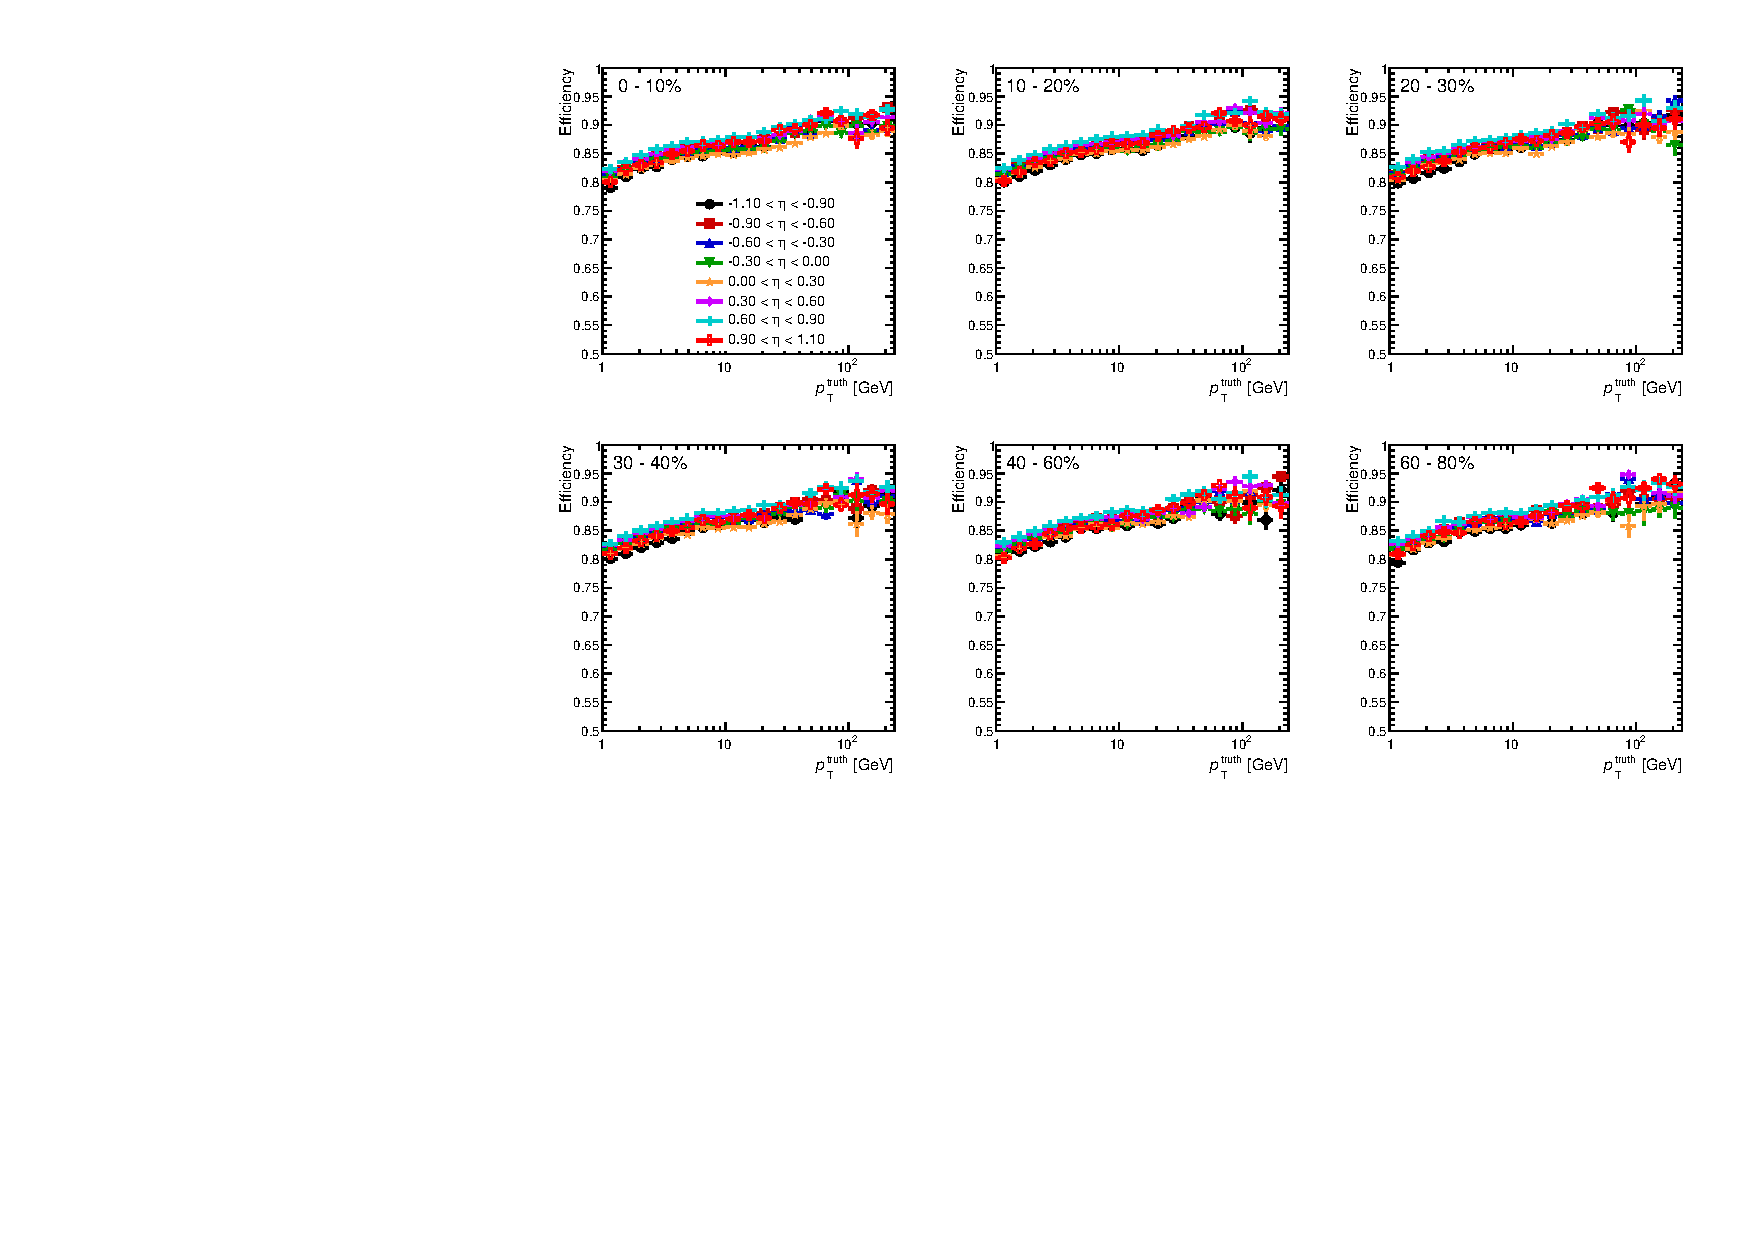
\includegraphics[width=0.7\textwidth]{figures/main/corrections/eff_cent_trketa_PbPb_ppTight.pdf}
\caption{Efficiency for reconstructing tracks evaluated using the default tracking selections in different track $\eta$ bins in the \pbpb\ MC overlay samples.
Each panel is a different centrality bin.}
\label{fig:pbpbeffdefault_final}
\end{figure}

\begin{figure}
\centering
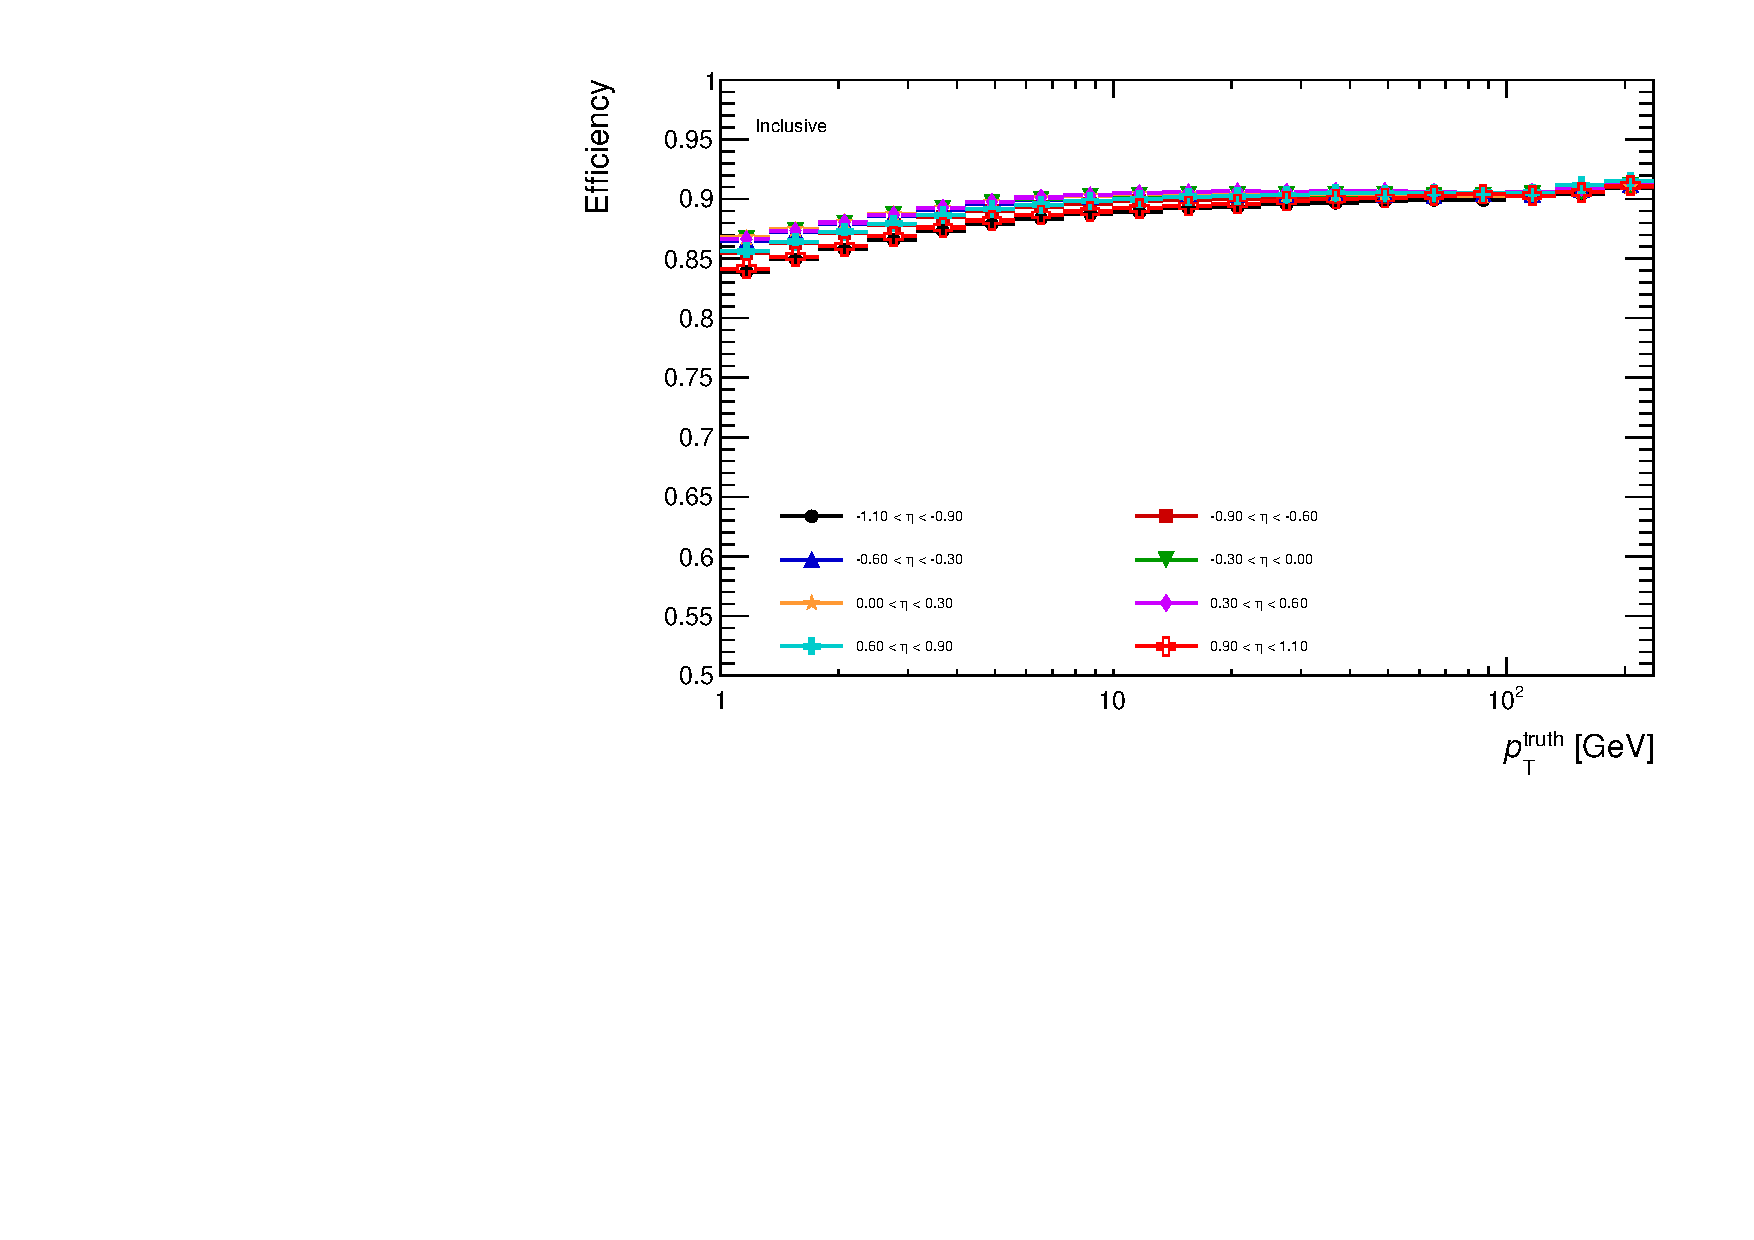
\includegraphics[width=0.45\textwidth]{figures/main/corrections/eff_cent_trketa_pp_ppTight.pdf}
\caption{Efficiency for reconstructing tracks evaluated using the default tracking selections in different track $\eta$ bins in the \pp\ MC samples.}
\label{fig:ppeffdefault_final}
\end{figure}

The final efficiency corrections applied were determined and applied as a function track \pt\ and track $\eta$, and can be seen in Figures~\ref{fig:pbpbeffdefault_final}-\ref{fig:ppeffdefault_final} for \pp\ and \PbPb\ collisions.
No significant dependence on the collision centrality is observed.
The efficiency exhibits a small, but monotonic increase with the track \pt.
Only a small variation with the track $\eta$ is observed in the region $|\eta|<1.1$.
The efficiency correction is applied on a track-by-track basis, assuming $\pttrk = \pTtrue$.
While that assumption is not strictly valid, the efficiency varies sufficiently slowly with $\pTtrue$ that the error introduced by this assumption is negligible, up to 1\%.
The tracking efficiency determined in Ref.~\cite{PhysRevC.98.024908} was not seen to be dependent on \ptjet\ for $\pttrk \lesssim 40$ GeV as can be seen in Figures~\ref{fig:pbpbeffdefaultjetpt_y0}-\ref{fig:ppeffdefaultjetpt}.
The small depletion of the efficiency for tracks with $\pt \sim 10-40$~GeV was attributed to the convolution of how jet fragments and with the performance of the track reconstruction in the dense core of the jet~\cite{PhysRevC.98.024908}.


\begin{figure}
\centering
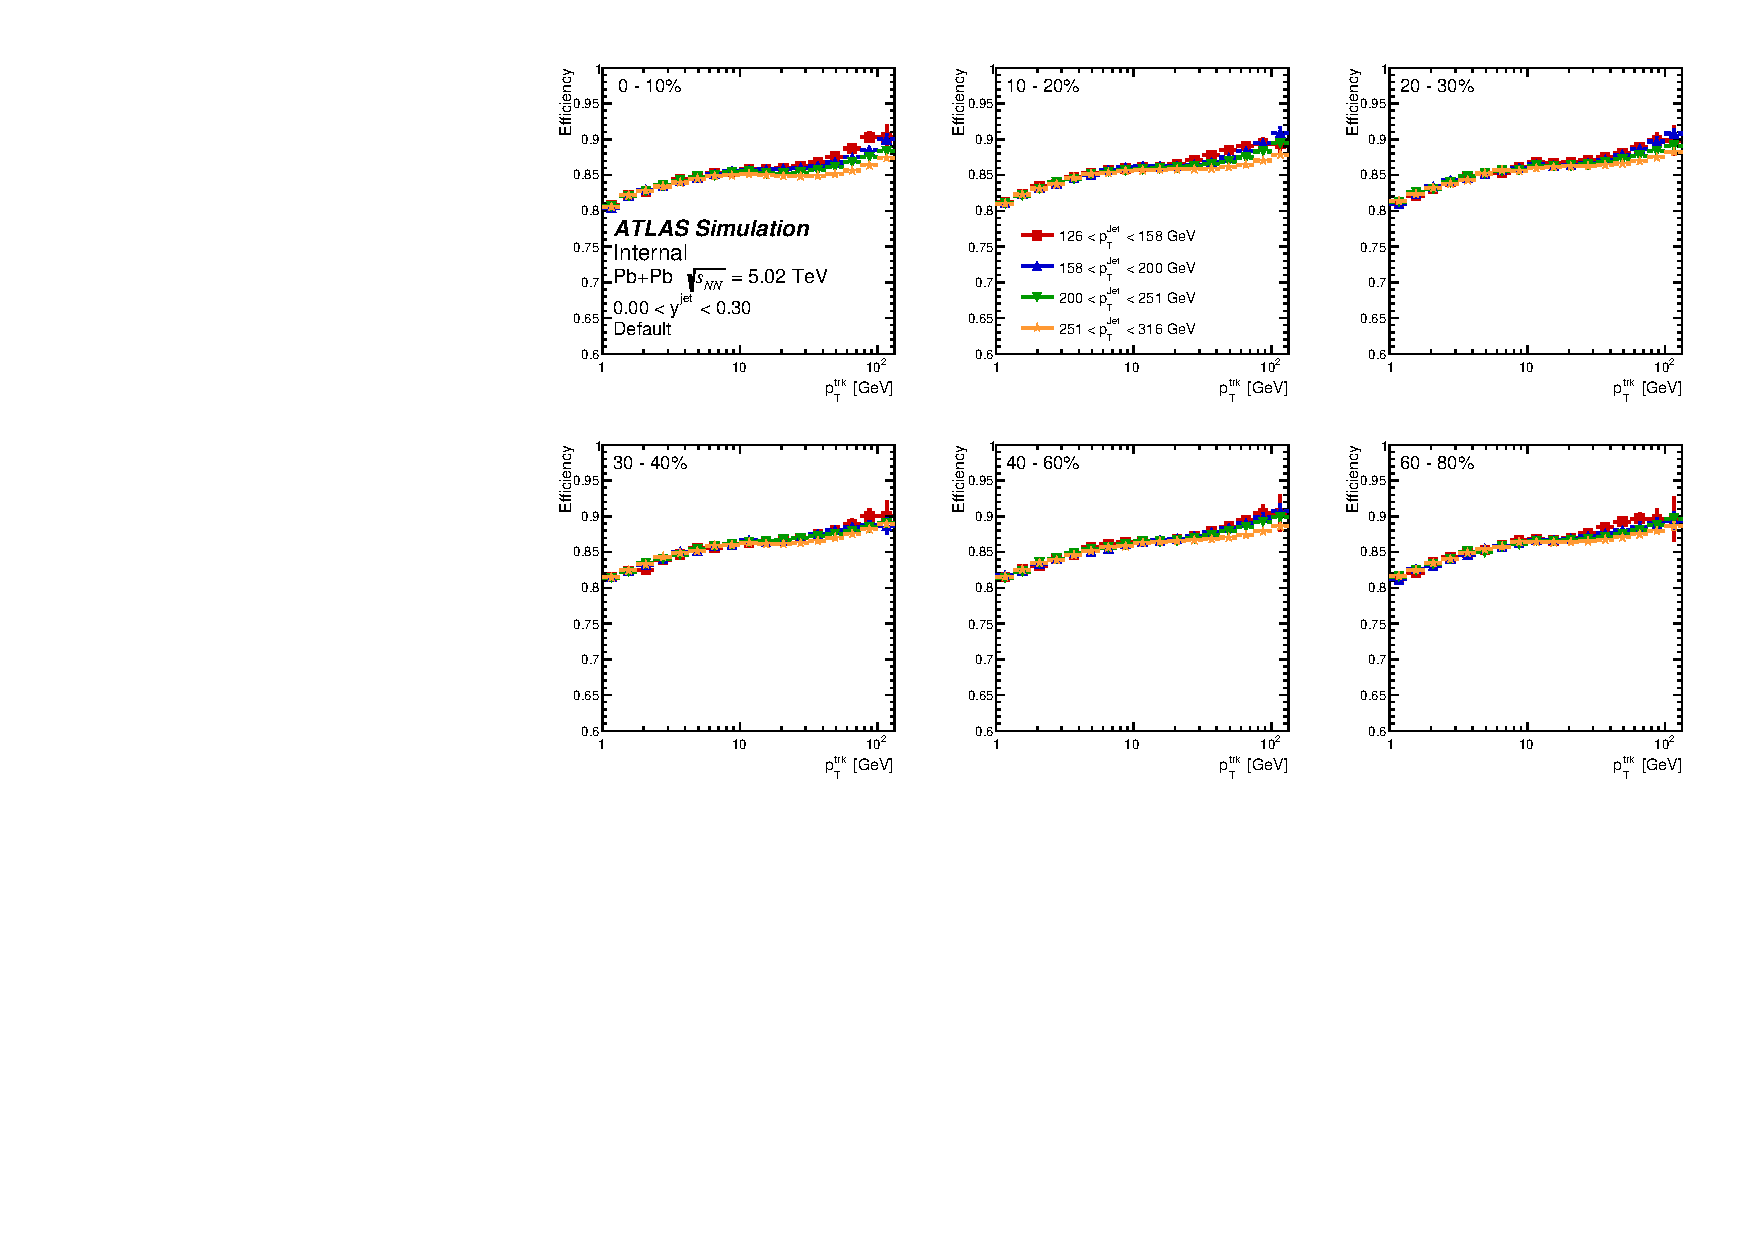
\includegraphics[width=0.7\textwidth]{figures/main/corrections/eff_centrality_jetpt_jety0_ppTight.pdf}
\caption{Efficiency for reconstructing tracks evaluated using the default tracking selections in different jet \pT\ bins and jet rapidity interval $|y|<0.3$ in the \pbpb\ MC overlay samples.
Each panel is a different centrality bin.}
\label{fig:pbpbeffdefaultjetpt_y0}
\end{figure}

\begin{figure}
\centering
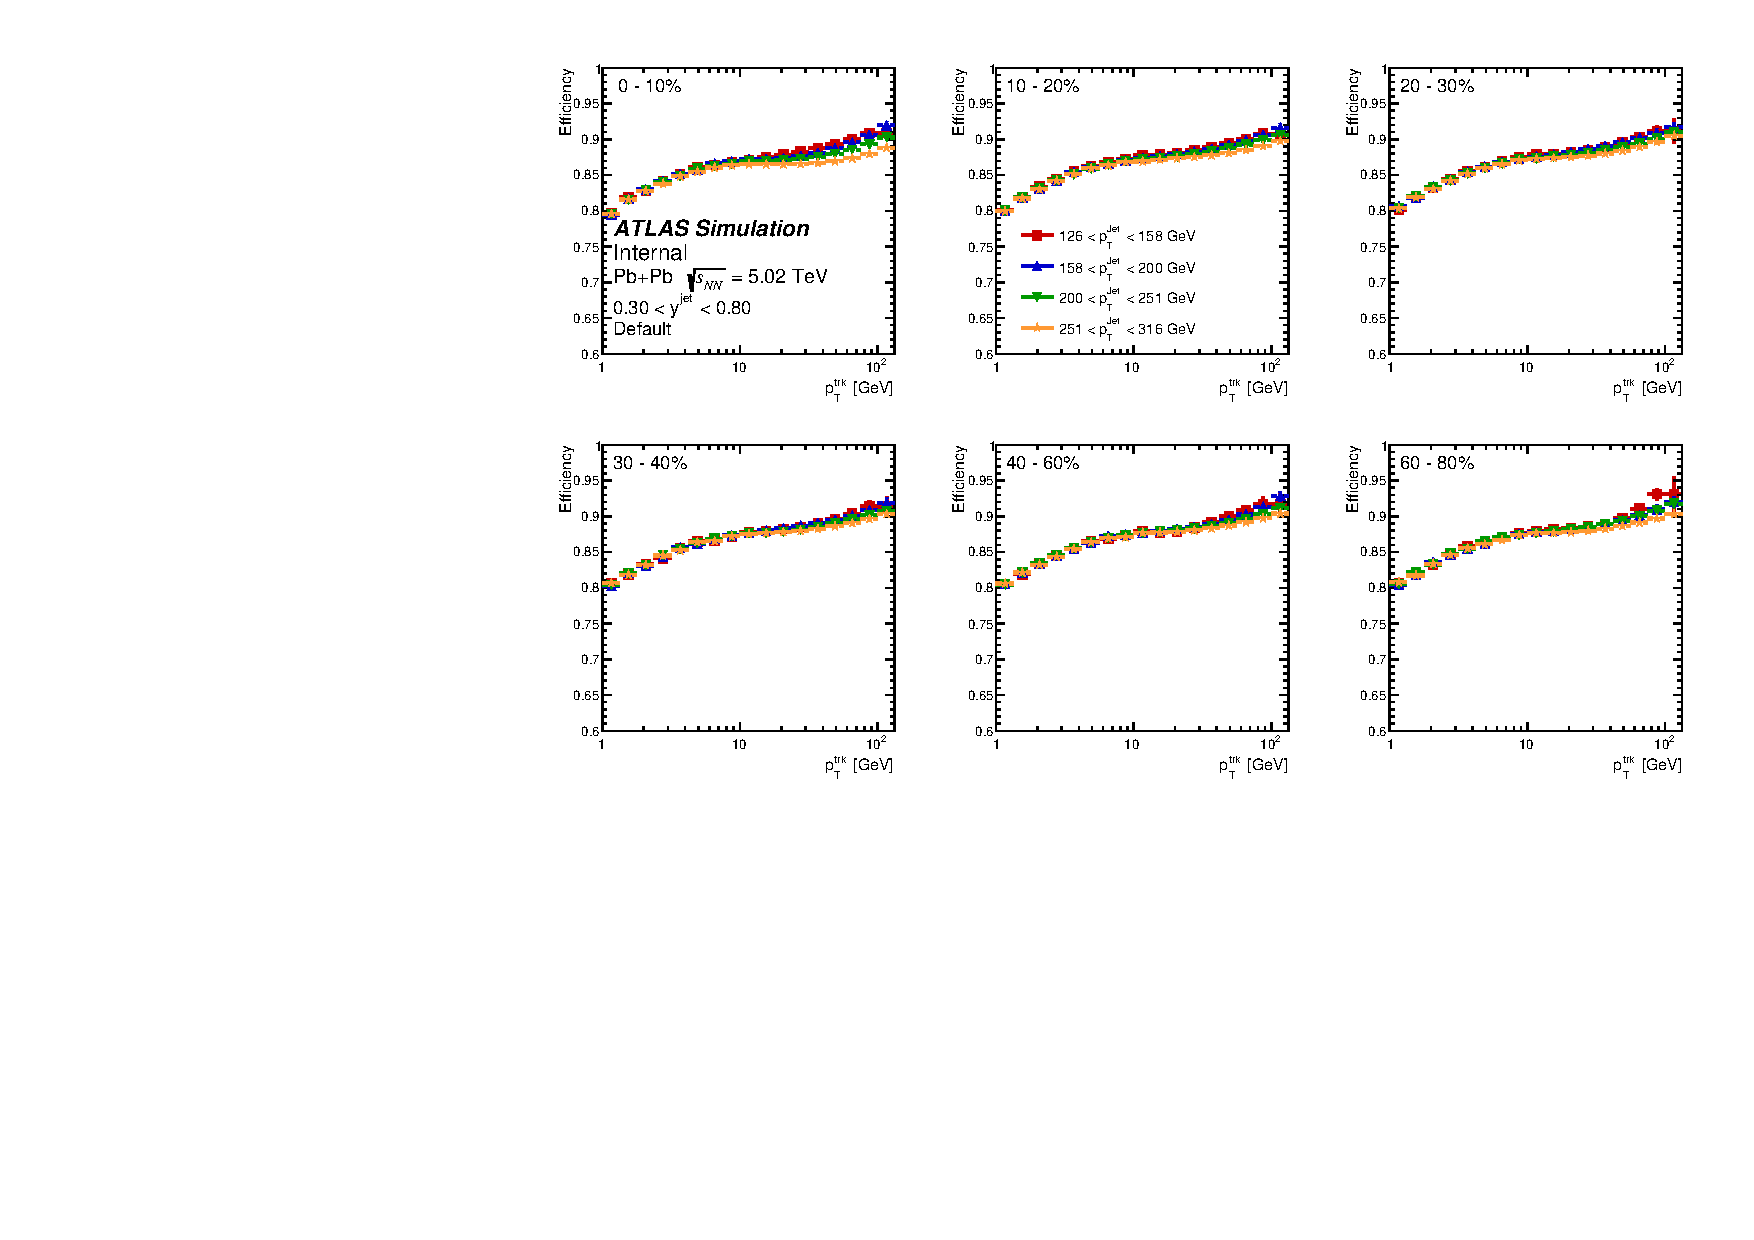
\includegraphics[width=0.7\textwidth]{figures/main/corrections/eff_centrality_jetpt_jety1_ppTight.pdf}
\caption{Efficiency for reconstructing tracks evaluated using the default tracking selections in different jet \pT\ bins and jet rapidity interval $0.3<|y|<0.8$ in the \pbpb\ MC overlay samples.
Each panel is a different centrality bin..}
\label{fig:pbpbeffdefaultjetpt_y1}
\end{figure}

\begin{figure}
\centering
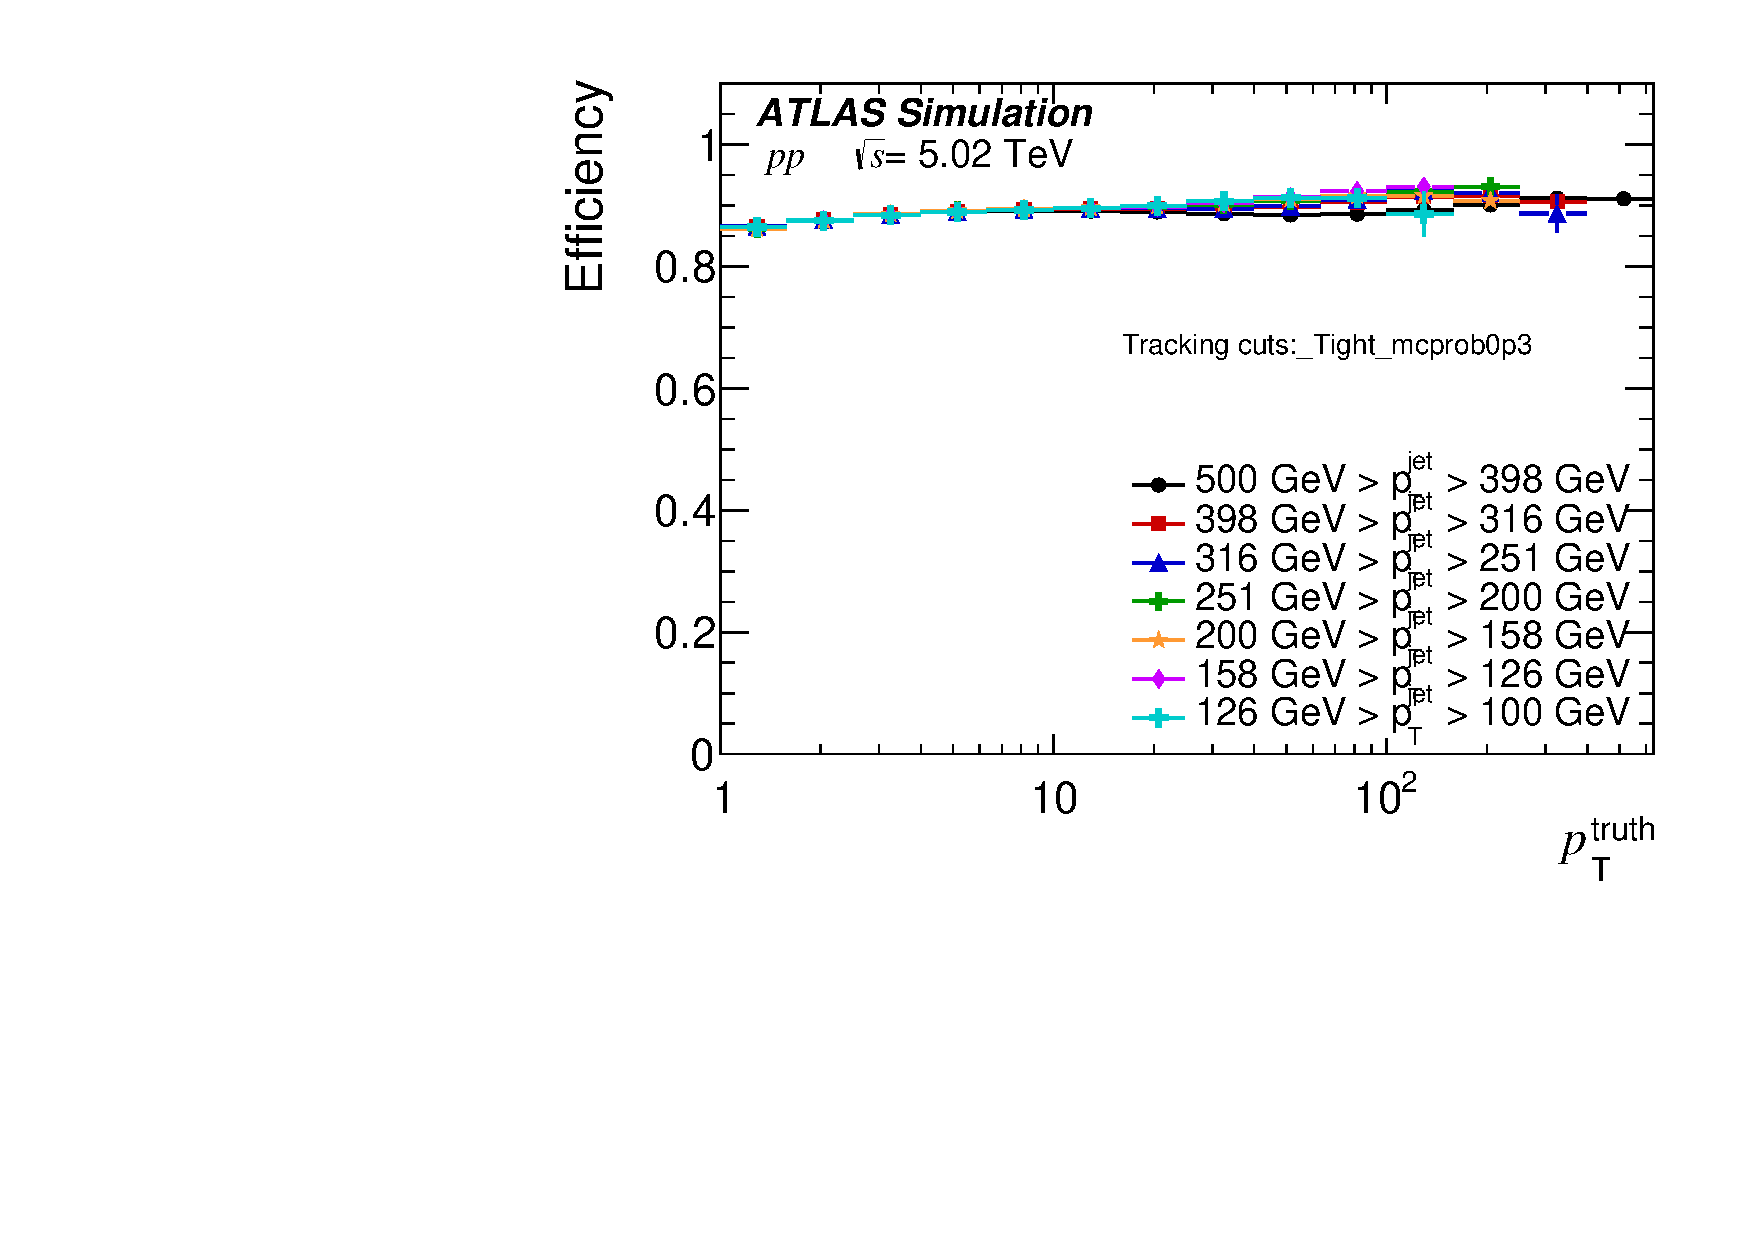
\includegraphics[width=0.45\textwidth]{figures/main/corrections/Trk_eff_v_pt_r005f_Tight_mcprob0p3_CX_Injet_0p0_0p3_pp_5p02.pdf}
\caption{Efficiency for reconstructing tracks evaluated using the default tracking selections in different jet \pT\ bins, in the \pp\ MC samples.}
\label{fig:ppeffdefaultjetpt}
\end{figure}

%%%%%%%%%%%%%%%%%%%%%%%%%%%%%%
\subsection{Fake rates}
\label{sec:fakerates}
Reconstructed tracks that cannot be matched to a primary particle in the MC samples or are matched to a secondary particle are considered to be ``fake'' tracks.
The rate of these tracks was evaluated and extensively studied in Ref.~\cite{PhysRevC.98.024908} in the \pp, \pbpb\ HIJING MC, and in \pbpb\ MC overlay samples.
The MC overlay sample is used to crosscheck the fake rate at higher \pt, but is not used for any corrections.
It was shown that as the \pttrk\ approaches the  \ptjet\ the fraction of fake tracks increases due to the steeply falling spectra of generator level tracks.
Figures~\ref{fig:fakeratepp} and \ref{fig:fakeratepbpb} show the fraction of tracks that are identified as fakes, secondaries, or part of UE in case of \PbPb\ collisions as a function of \pttrk\ for selections in \ptjet in \pp\ and \pbpb\ collisions, respectively.
The rate decreases with \pttrk\ up to approximately 10~GeV and then remains constant until \pttrk\ approaches \ptjet\ where the rate increases again.
In \pbpb\ collisions, the ``fake'' rate also includes tracks which are from the underlying event from the real collisions into which the jet is overlaid.
The rate of these underlying event tracks increases with decreasing \pttrk\ and increasing collision centrality.
The contribution from UE is negligible for tracks with \pT\ above 10 GeV as no centrality dependence is seen.
The Figure~\ref{fig:fakeratepbpb} excludes the very low \pT\ region where the distribution would be completely dominated by the UE.
The size of the UE is then presented further in Figure~\ref{fig:UEimpact}.
To separate the contribution of UE tracks (see section~\ref{sec:cuts_UE}) from the fake tracks in \PbPb\ collisions and cross-check the centrality dependence of the fake rate, 200,000 MB \PbPb\ fully reconstructed HIJING MC~\cite{Wang:1991hta} events were used.
The HIJING MC generator is capable of simulating global properties of HI collisions.
The estimated fake rate of tracks associated with jets with $\pT>40$ GeV is at the level of 1\% and it exhibits similar behavior as observed in Figure~\ref{fig:fakeratepbpb}.
No significant dependence of the fake rate on the collision centrality was found~\cite{PhysRevC.98.024908}.

\begin{figure}
\centering
\begin{tabular}{cc}
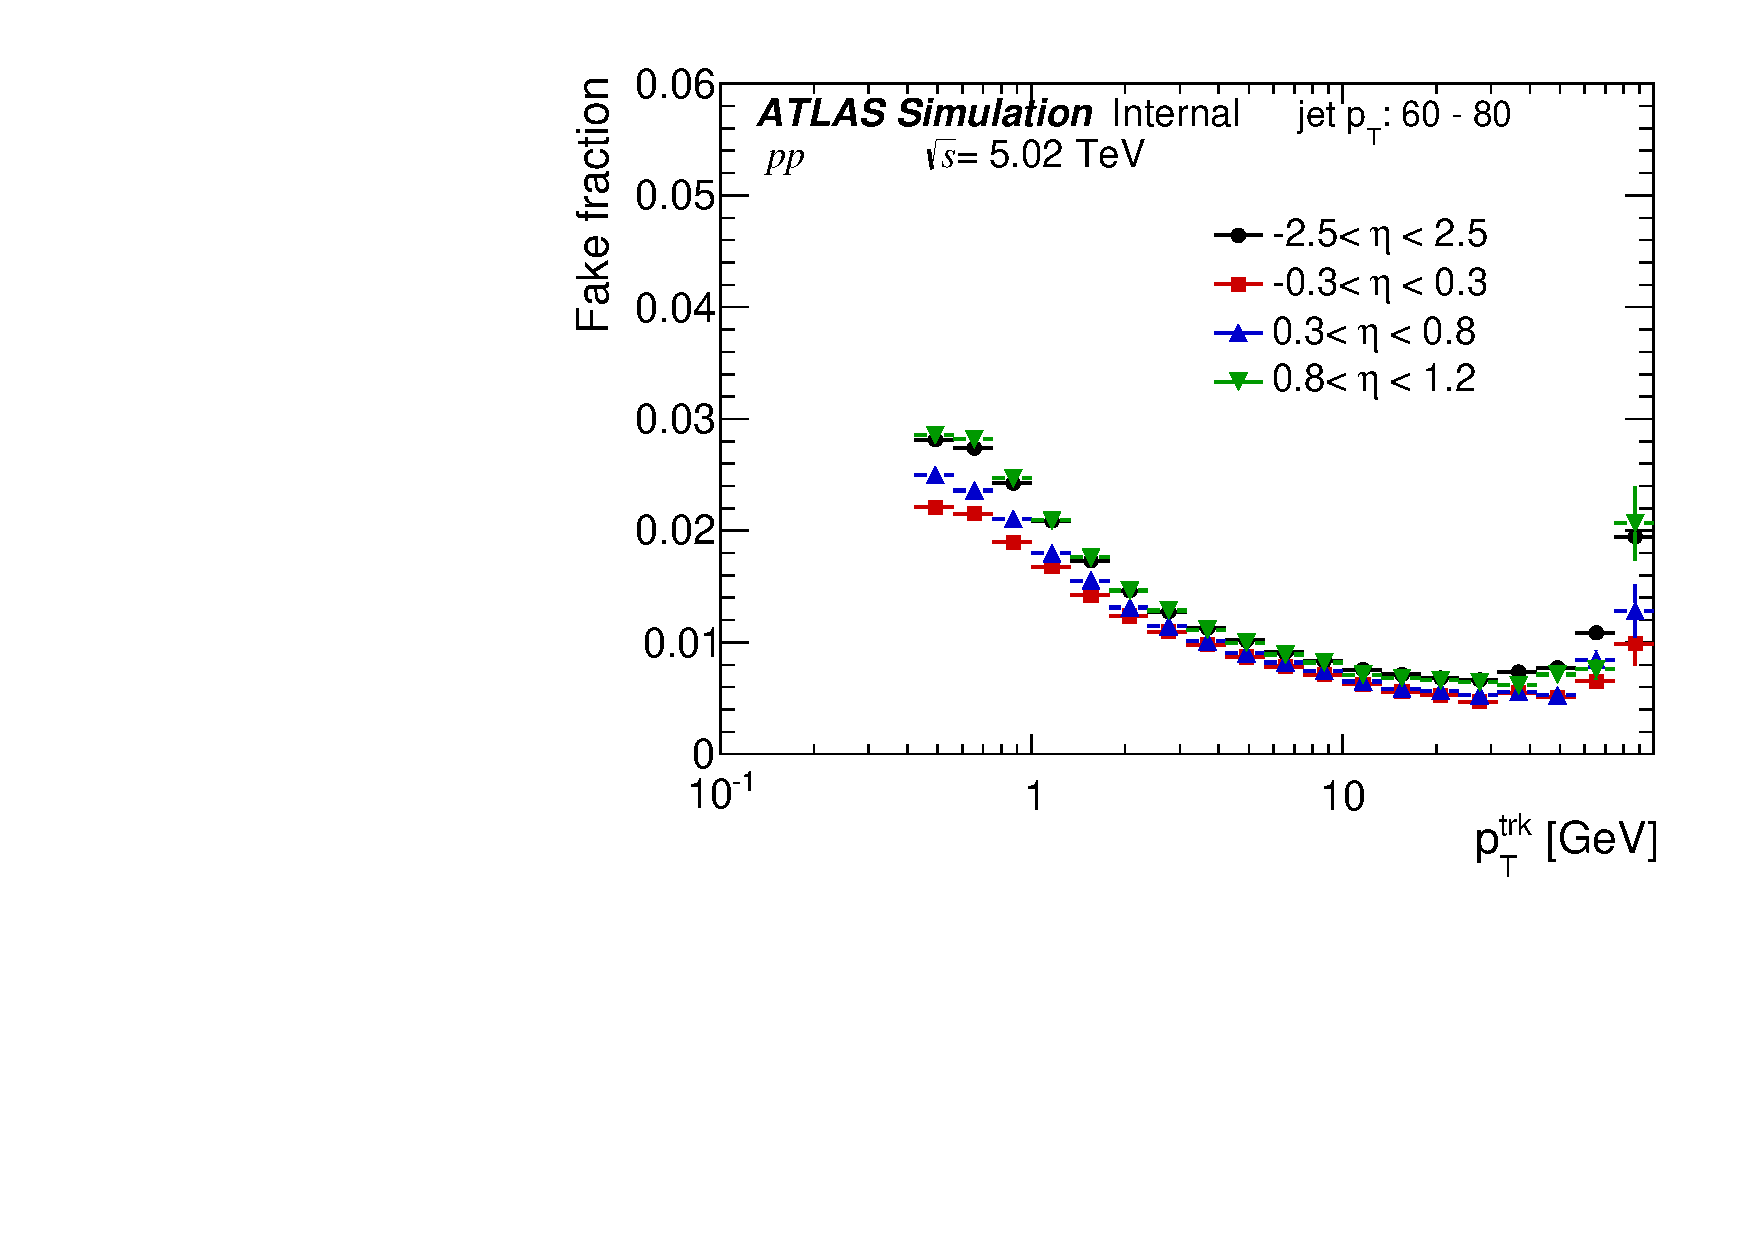
\includegraphics[width=0.45\textwidth]{figures/main/corrections/fake_rates/FakesEta_pp_5p02_r003_Tight_mcprob0p3_JZ2_jetpt_2.pdf} &
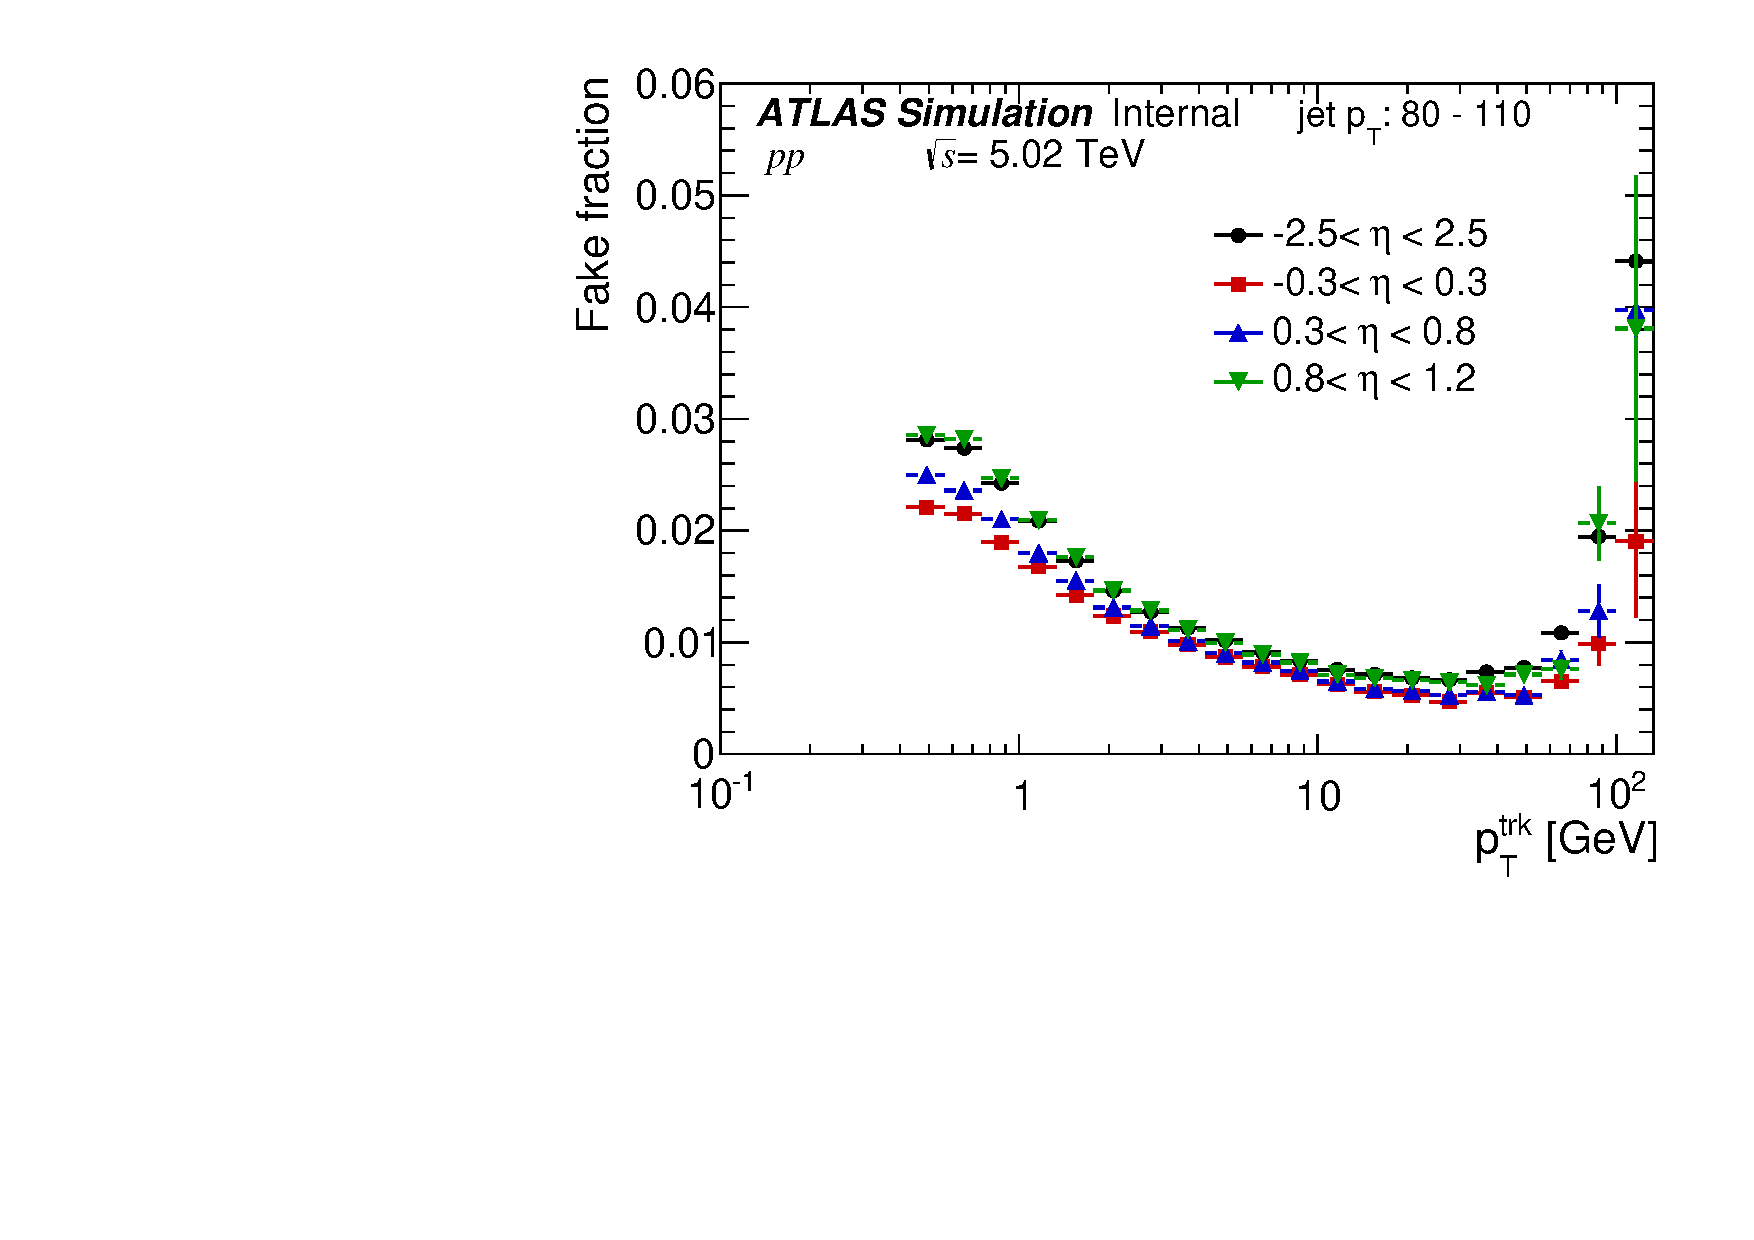
\includegraphics[width=0.45\textwidth]{figures/main/corrections/fake_rates/FakesEta_pp_5p02_r003_Tight_mcprob0p3_JZ2_jetpt_3.pdf} \\
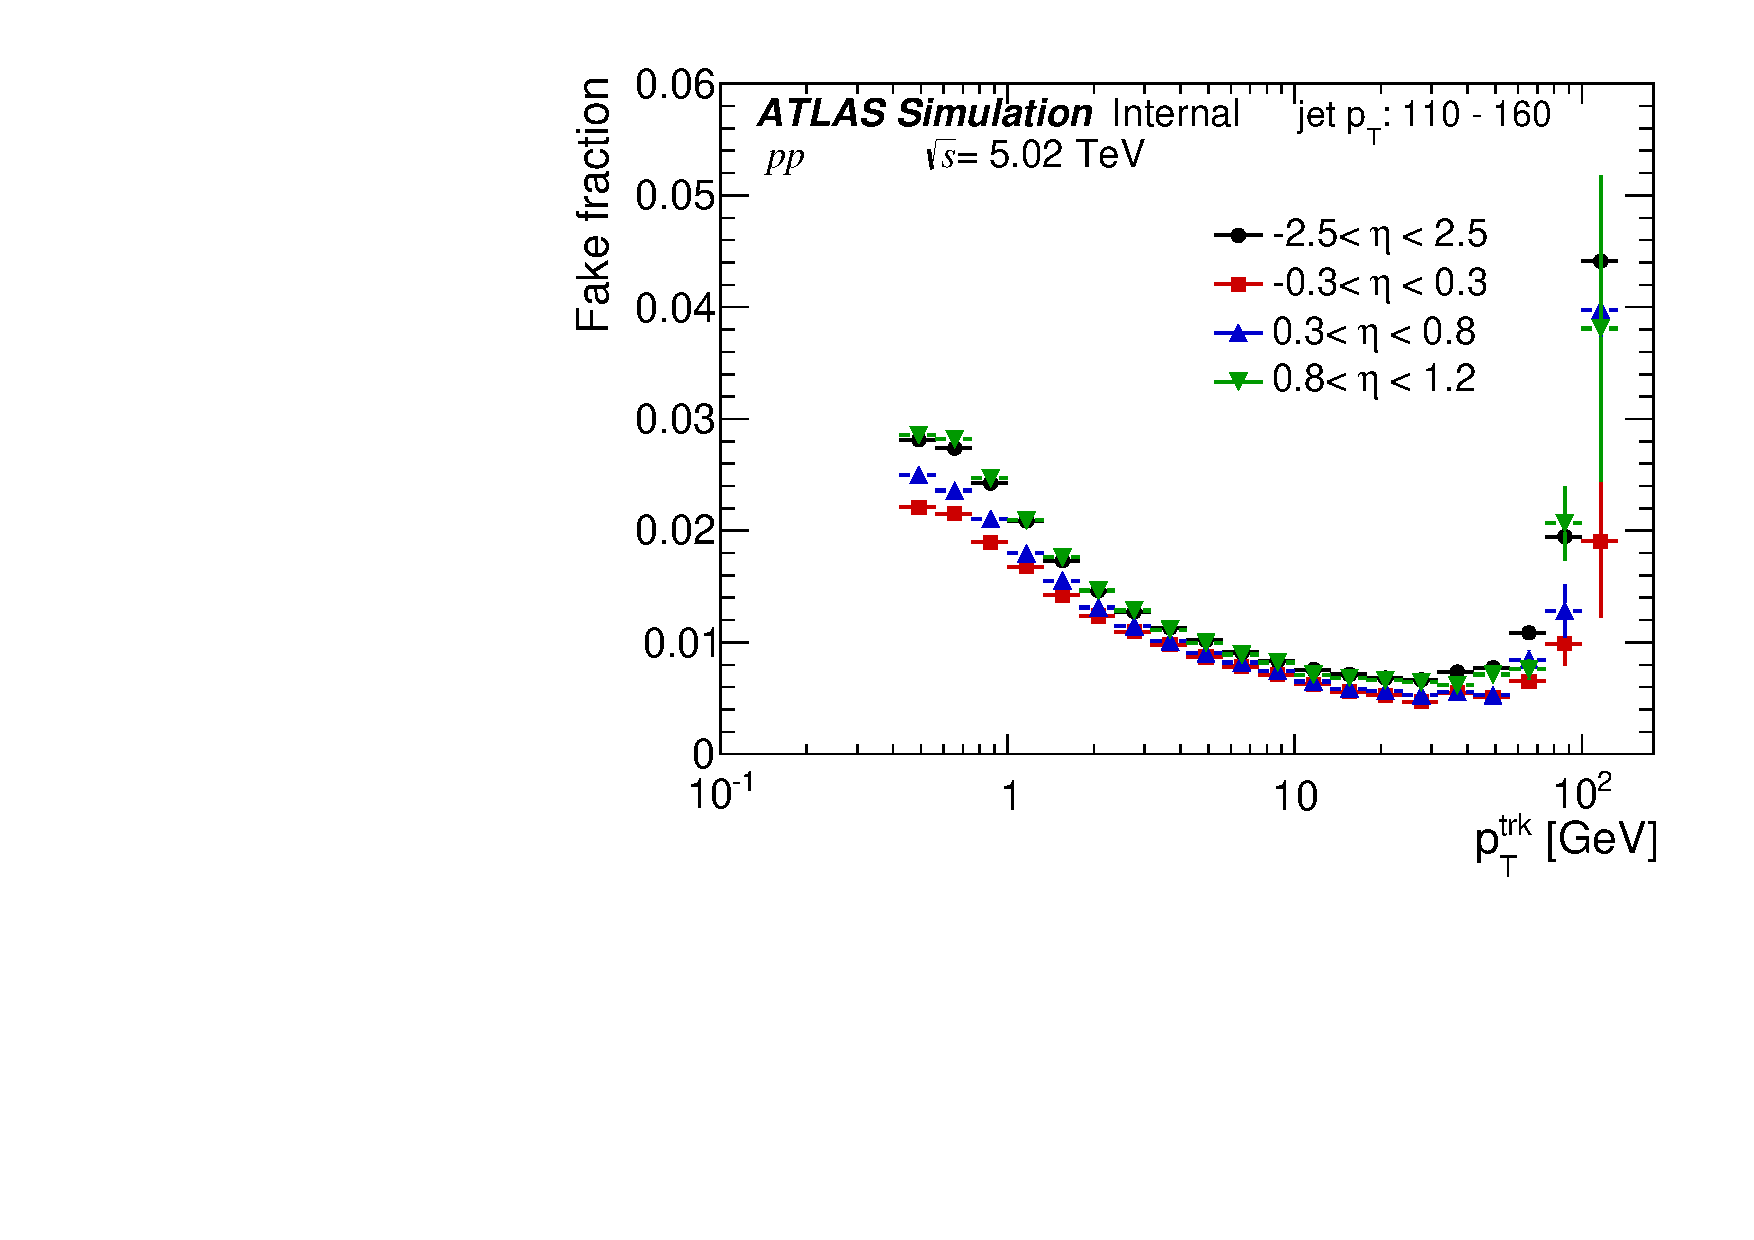
\includegraphics[width=0.45\textwidth]{figures/main/corrections/fake_rates/FakesEta_pp_5p02_r003_Tight_mcprob0p3_JZ2_jetpt_4.pdf} &
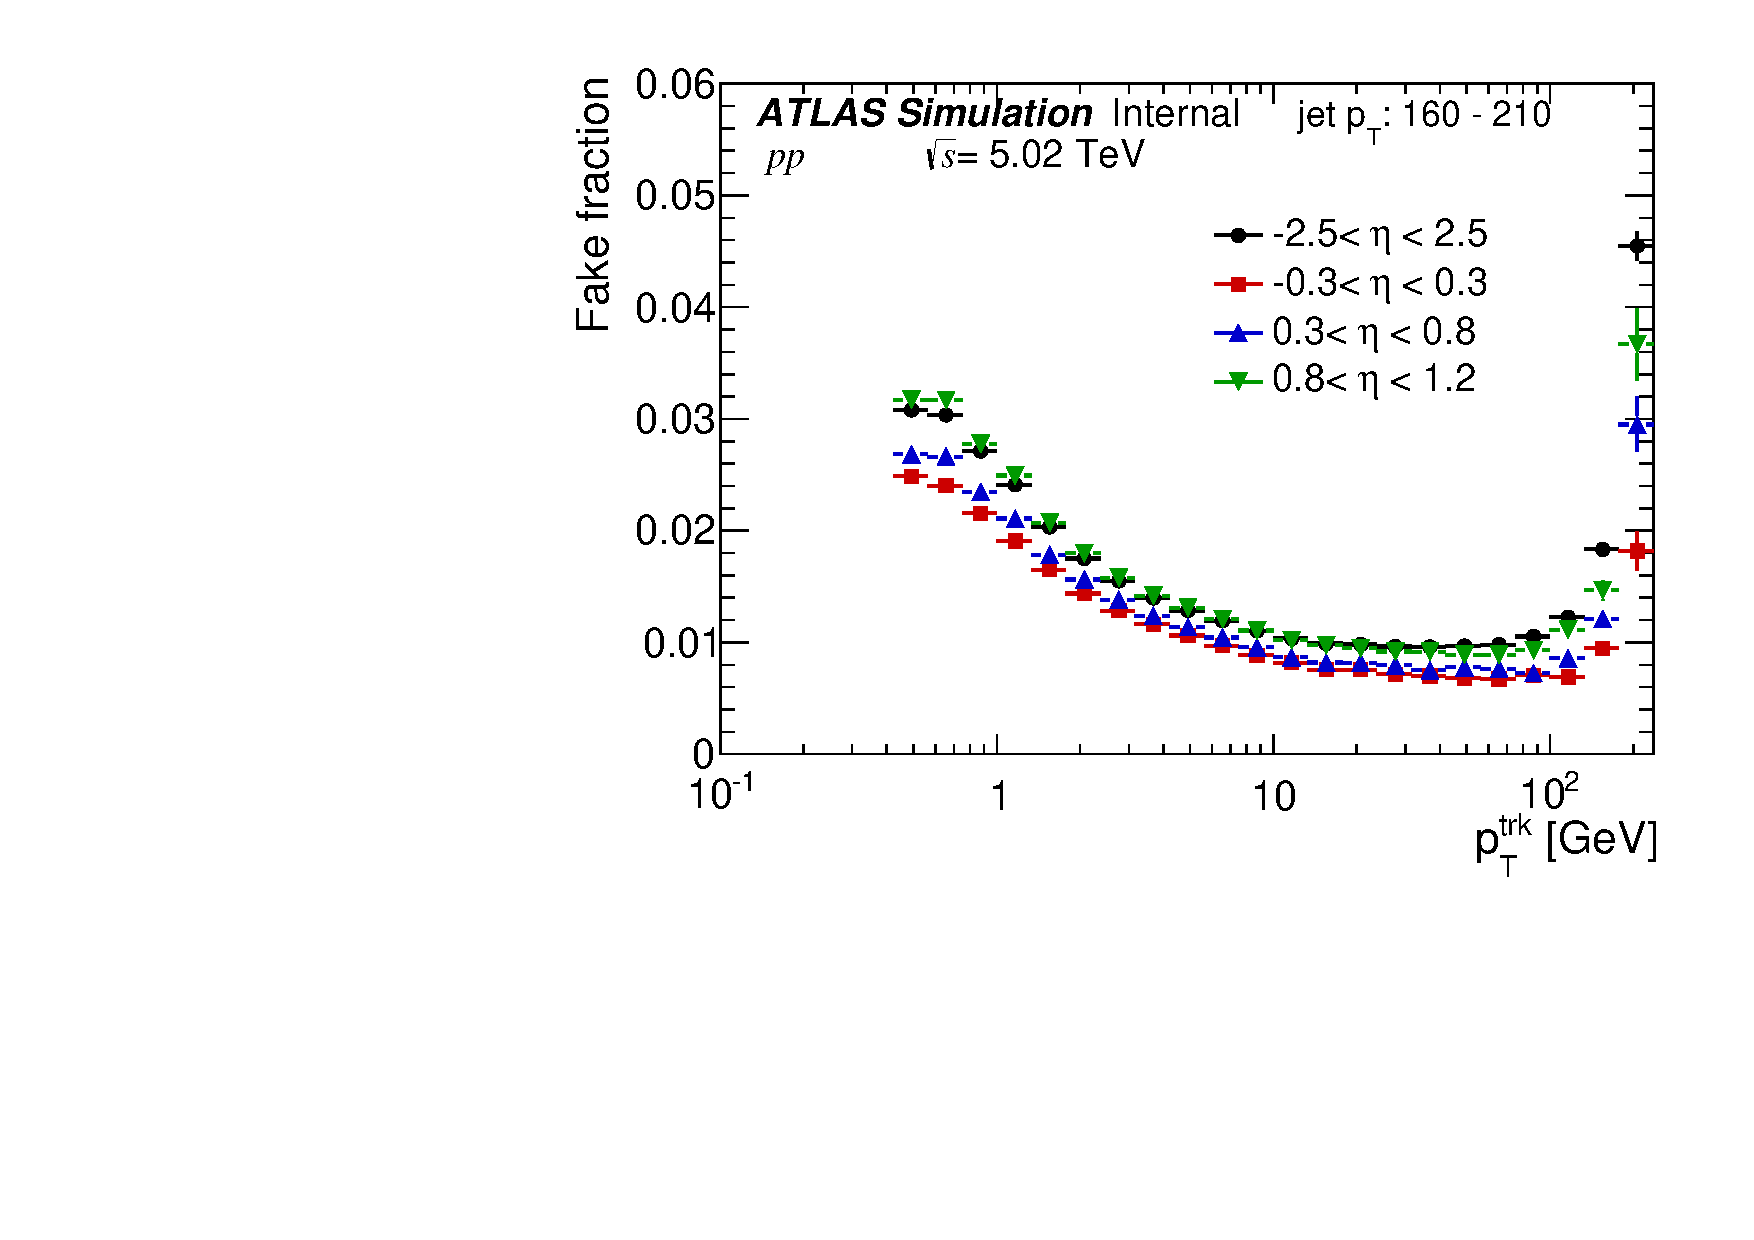
\includegraphics[width=0.45\textwidth]{figures/main/corrections/fake_rates/FakesEta_pp_5p02_r003_Tight_mcprob0p3_JZ3_jetpt_5.pdf} \\
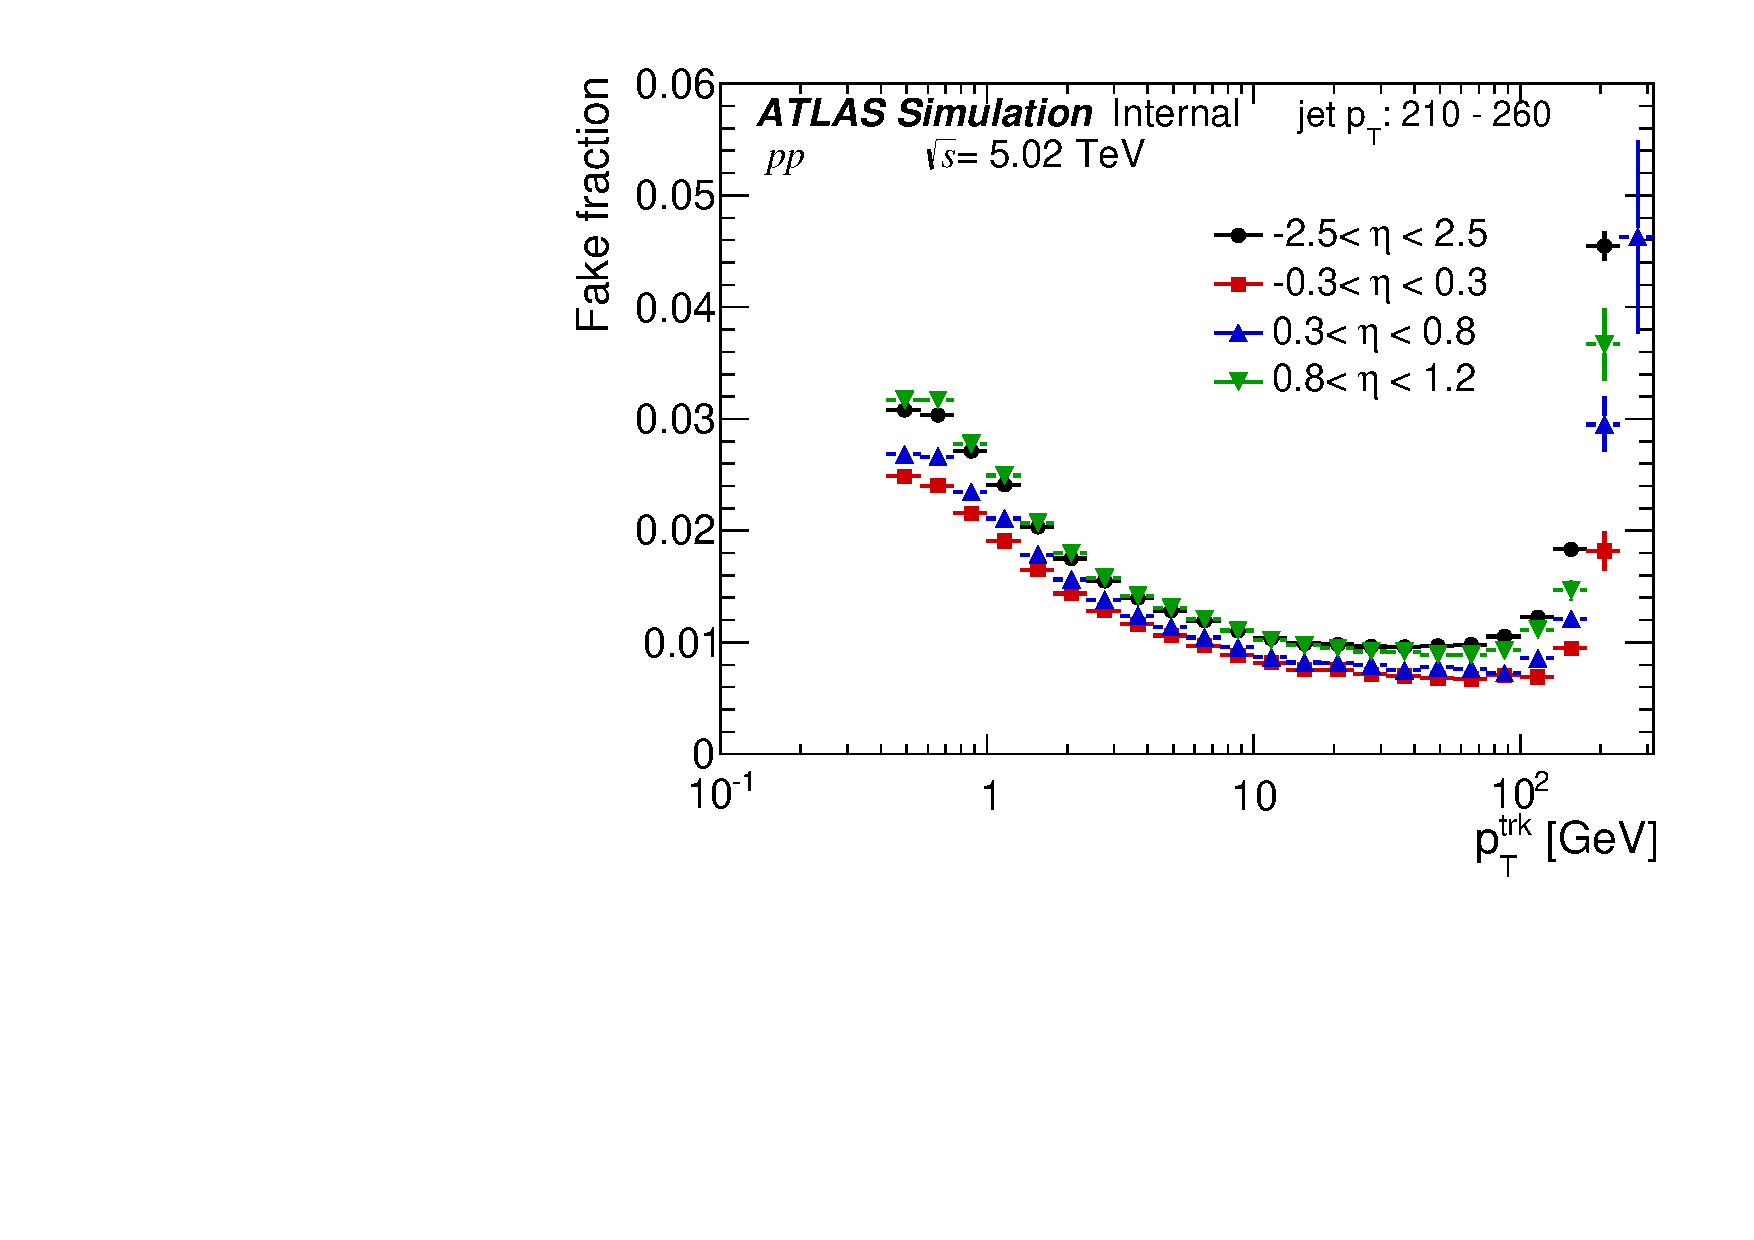
\includegraphics[width=0.45\textwidth]{figures/main/corrections/fake_rates/FakesEta_pp_5p02_r003_Tight_mcprob0p3_JZ3_jetpt_6.pdf} &
\end{tabular}
\caption{Fake rate for five different \ptjet\ selections in 5.02 TeV \pp\ collisions and four pseudorapidity intervals.
The fake rate is evaluated for default value of \mcprob\ cut of 0.3 used in 2015 analysis.
Figure from Ref.~\cite{Sickles:2235420}.}
\label{fig:fakeratepp}
\end{figure}  

\begin{figure}
\centering
\begin{tabular}{cc}
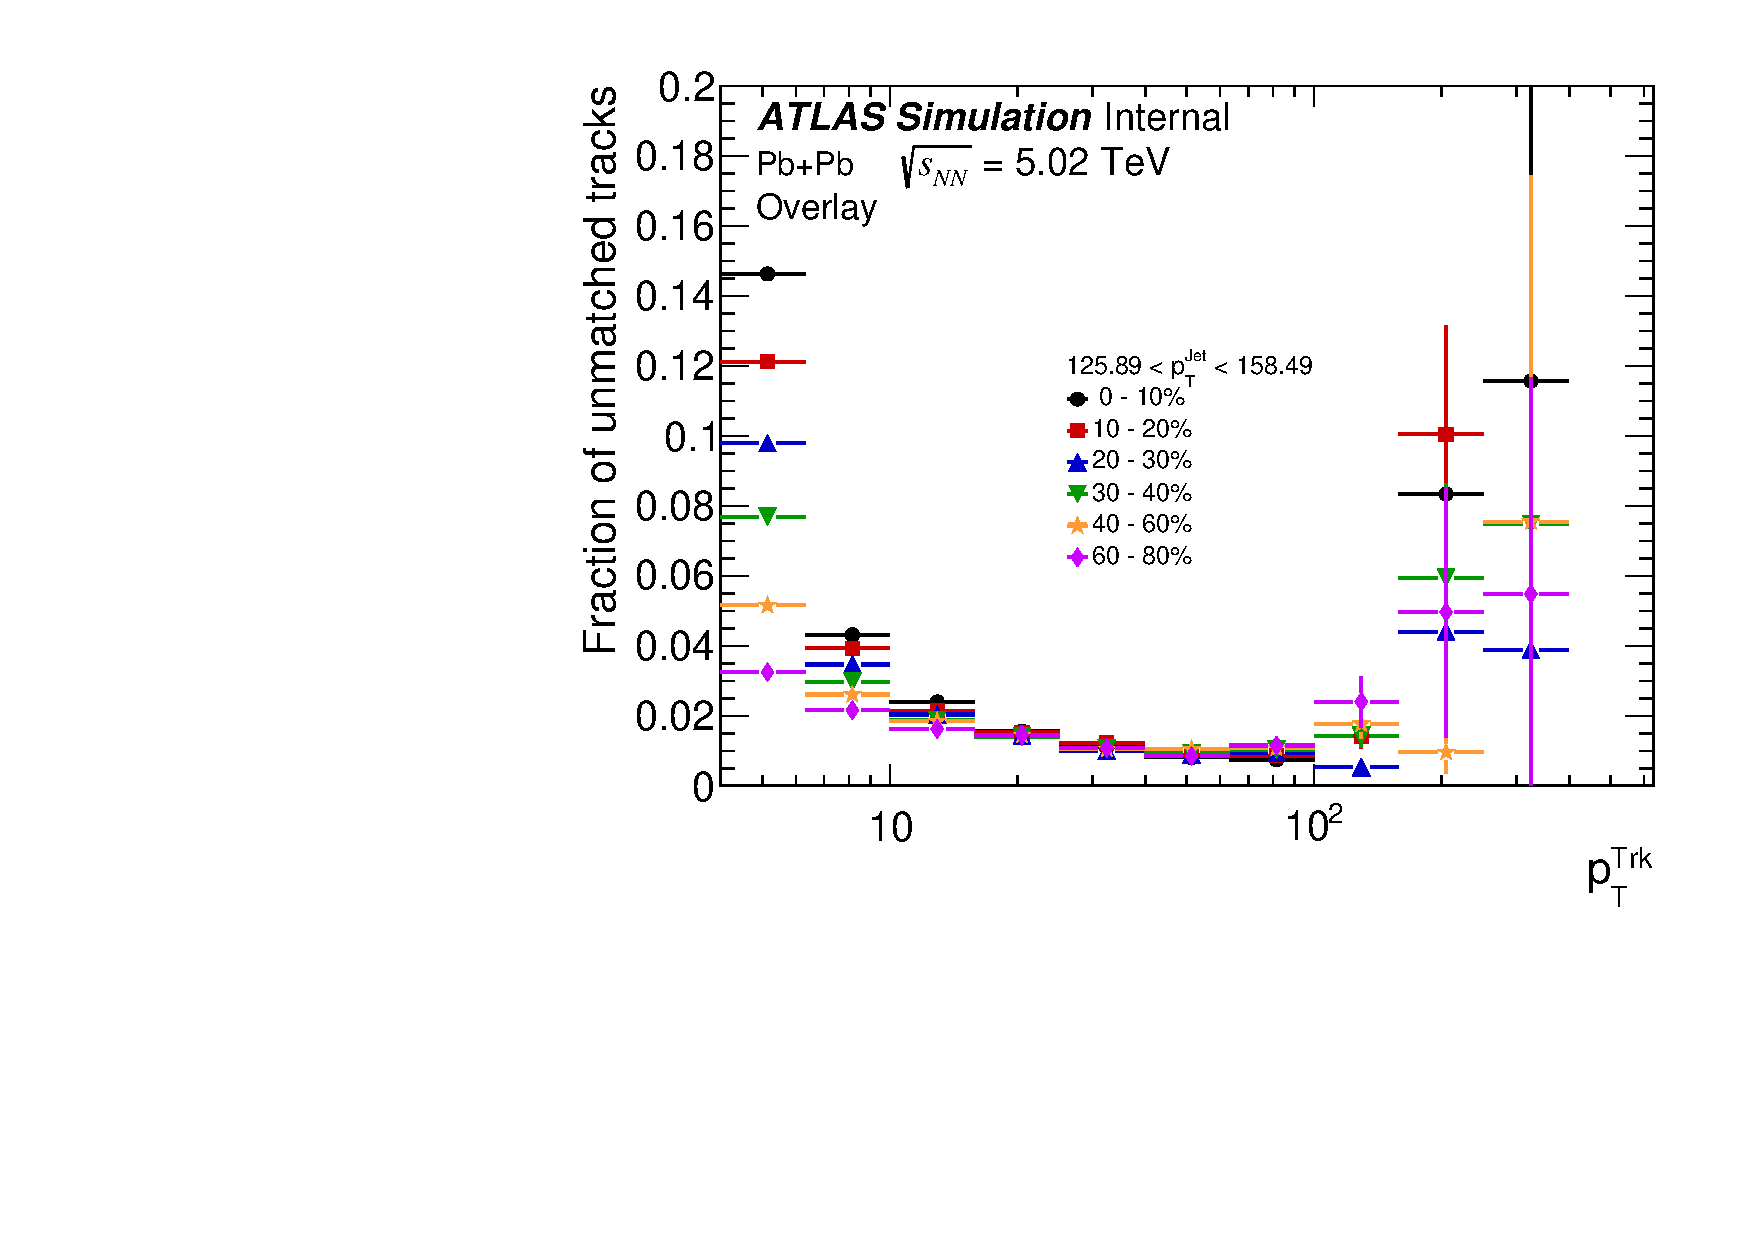
\includegraphics[width=0.45\textwidth]{figures/main/corrections/fake_rate_pt_125GeV.pdf} &
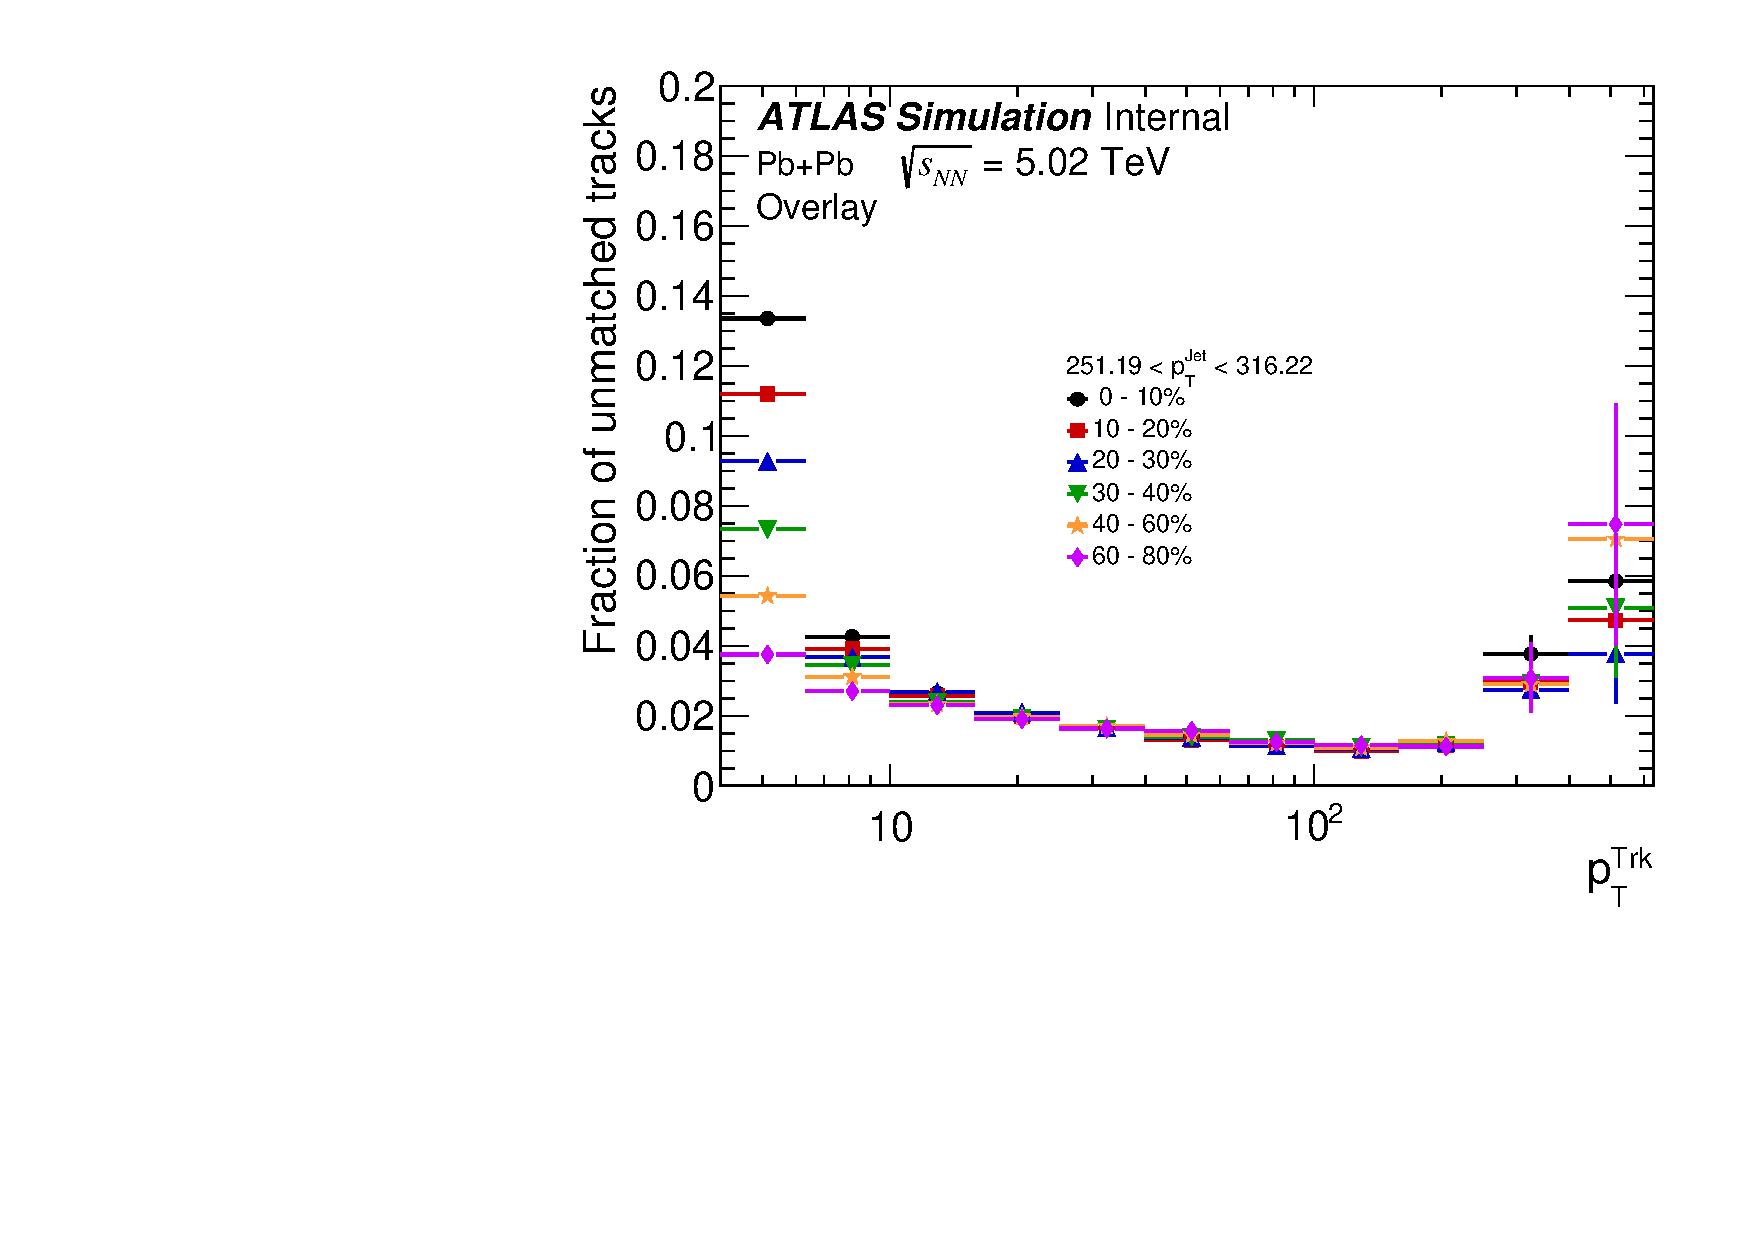
\includegraphics[width=0.45\textwidth]{figures/main/corrections/fake_rate_pt_251GeV.pdf} \\
\end{tabular}
\caption{ Rate of tracks unmatched to truth tracks
in \pbpb\ collisions for different centrality selections as indicated on the plot as a function of \pttrk.
The unmatched tracks include both fake tracks and tracks from the underlying event.
The panels show two \ptjet\ selections: 126-158~GeV (left) and 251-316~GeV (right).
The low \pT\ part is omitted as it is dominated by the contribution from the UE.
Figure from Ref.~\cite{Sickles:2235420}.}
\label{fig:fakeratepbpb}
\end{figure}
\begin{figure}
\centering
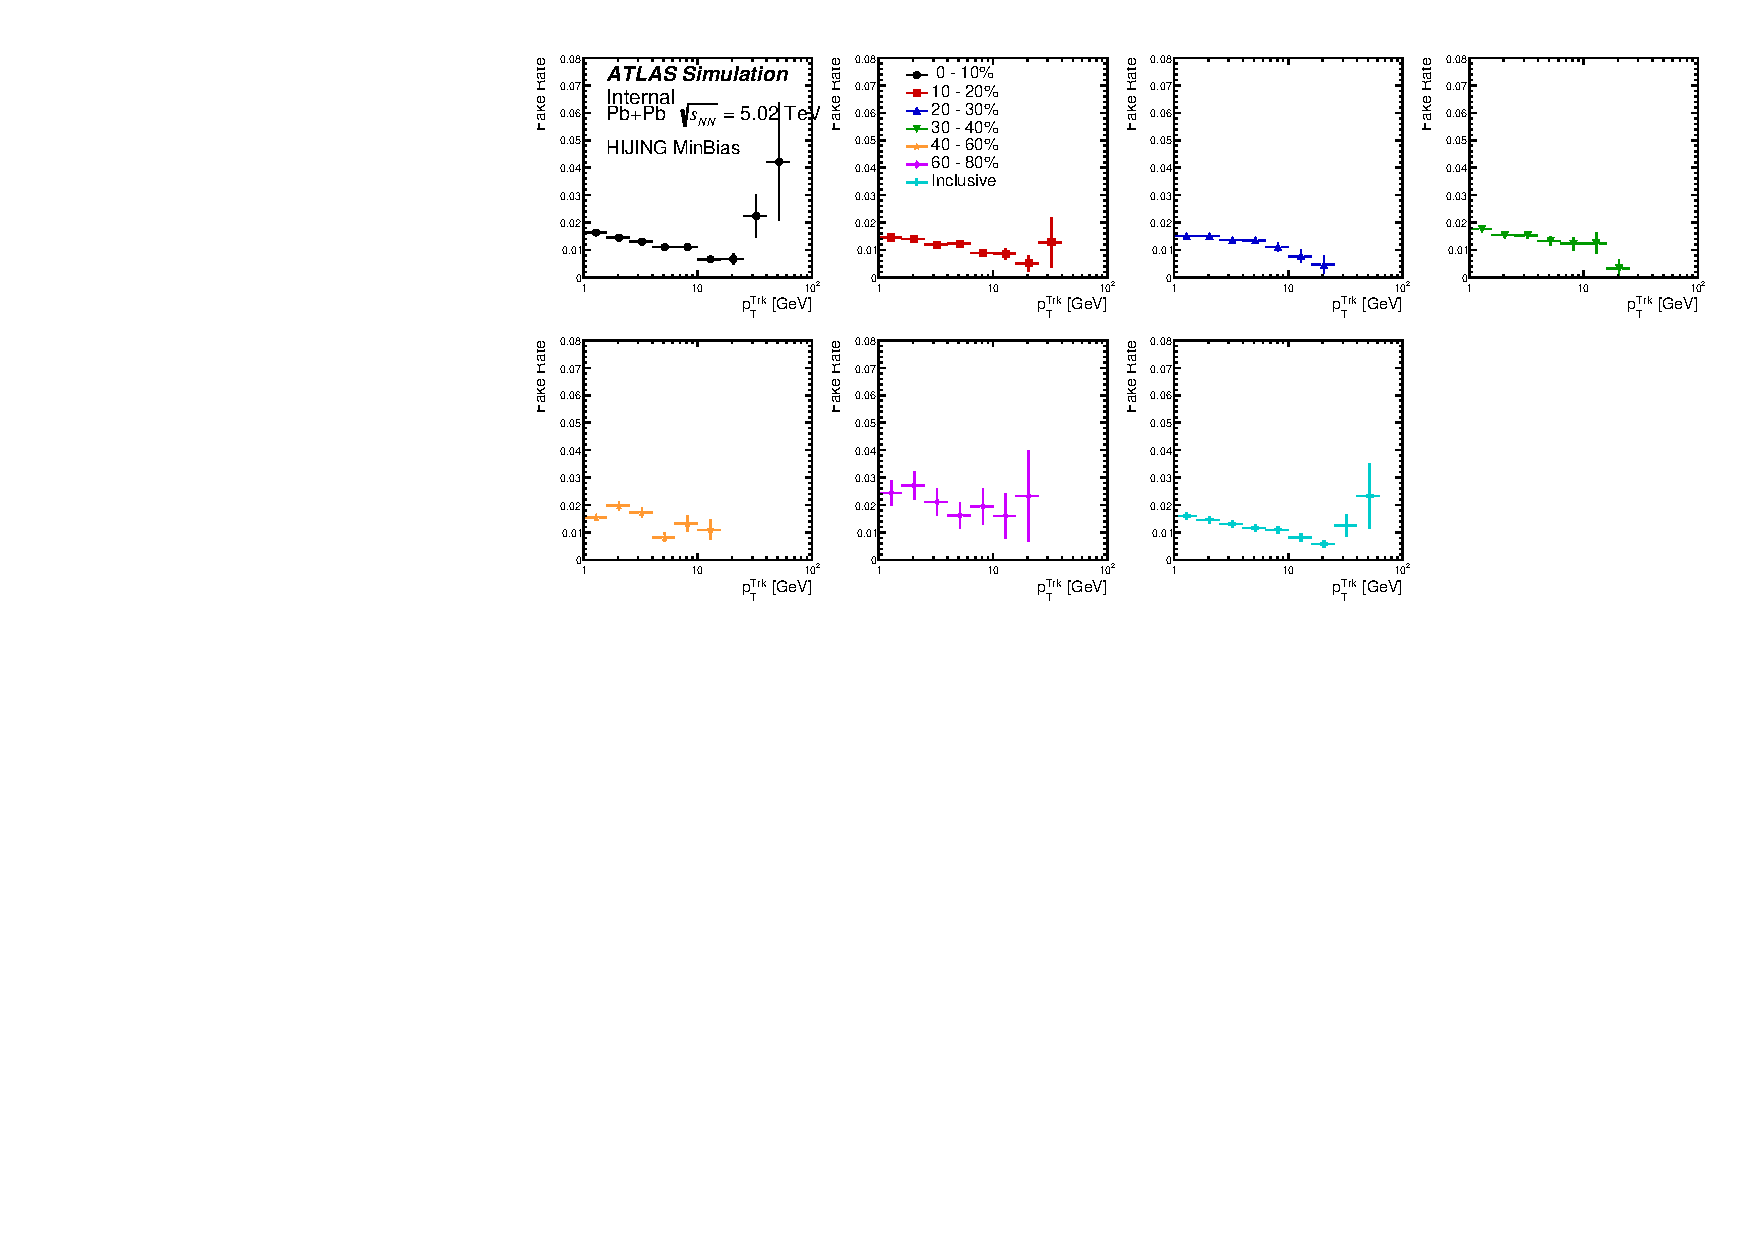
\includegraphics[width=1.\textwidth]{figures/main/performance/fake_rate_hijingMB.pdf}
\caption{ Fake rate for six different centrality intervals in 5.02 TeV \pbpb\ HIJING MC collisions.
The fake rate is evaluated for default value of $\mcprob = 0.3$ in 2015 analysis.}
\label{fig:fakeratehijing}
\end{figure}


To correct for the contribution from fake and secondary particles, charged particle distributions are estimated using reconstructed tracks that do not have a truth match as defined by criteria described in previous paragraphs.
These distributions are then subtracted from the measured distributions both in the data and MC.
This procedure is applied for tracks above 10 GeV in \PbPb\ collisions and for tracks above 1 GeV in \pp\ collisions.
The correction also removes any residual UE above 10~GeV in case of \PbPb.
The choice of the 10 GeV cut is based on the centrality dependence of the rate of truth-unmatched tracks in MC overlay samples shown in Figure~\ref{fig:fakeratepbpb}.
The correction for UE, fake and secondary tracks below 10 GeV in \PbPb\ collisions is discussed in the next section.


%%%%%%%%%%%%%%%%%%%%%%%%%%%%%%
\subsection{Underlying event subtraction of tracks}
\label{sec:cuts_UE}
Charged particles from the nucleon-nucleon scatterings that are not associated with the hard scattering in question constitute a background to the \Dptr\ distributions that needs to be subtracted from the measured distributions.
This background strongly depends on the collisions centrality and on the charged particle \pt.
In the measurement of the inclusive jet fragmentation functions it was found that the UE contribution is negligible for charged particles with $\pt>10$~GeV~\cite{PhysRevC.98.024908}.
This can be seen in the centrality dependence of the combined rate of fake and underlying event charged particles shown in Figure~\ref{fig:fakeratepbpb} where no significant centrality dependence is observed for track above 10 GeV.

In \pp\ collisions, the UE is not subtracted.
The pileup contribution is negligible and subtracting the intrinsic UE from the hard scattering processes would also necessitate a similar subtraction in the particle level fragmentation functions in \pbpb\ that would be generator dependent and make comparisons between \pp\ and \pbpb\ non-trivial.

In \pbpb\ collisions, the UE from the soft processes is estimated using two independent methods.
The ``Map method" is nominally used for the analysis while the ``Cone method" is used to provide a systematic uncertainty.
The former uses charged particle distributions of $\mathrm{d}N_{\mathrm{ch}}/\mathrm{d}\phi\mathrm{d}\eta(\mathrm{cent},\pt, \mathrm{d}\Psi_{\mathrm{ch}})$ in MC overlay events, while the latter evaluates the underlying event on an event-by-event basis using a grid of cones.

%%%%%%%%%%%%%%%
\subsubsection{Map Method}
\label{sec:map_method}
In the "Map Method", $\eta-\phi$ maps of the average number of UE charged particles in a given annulus around a jet ($\nchUE^{\mathrm{Map}}$) are determined in MC overlay events using tracks without a truth match.
The maps are filled as a function of the distance from the jet, \ptjet, \etajet, \phijet, angle of the jet to the reaction plane\footnote{The reaction plane angle $\Psi$ is determined on an event-by-event basis by a standard method using the $\phi$ variation of transverse energy in the forward calorimeter} $ \mathrm{d}\Psi_{\mathrm{ch}}$, \pt\ and centrality.

Examples of the these distributions for three different annuli (0--0.05, 0.25 -- 0.30, 0.60--0.70), in the $\mathrm{d}\Psi$ interval of  0.80 -- 1.00, for six collision centrality classes and for 1--1.6 GeV particles in 126 -- 158 GeV jets are shown in Figure~\ref{fig:ue_map}.
The number of UE particles associated with a jet decreases with size of the annulus, decreasing centrality, increasing track \pT\ and increasing distance to the reaction plane.

\begin{figure}
\begin{subfigure}{.5\textwidth}
\centering 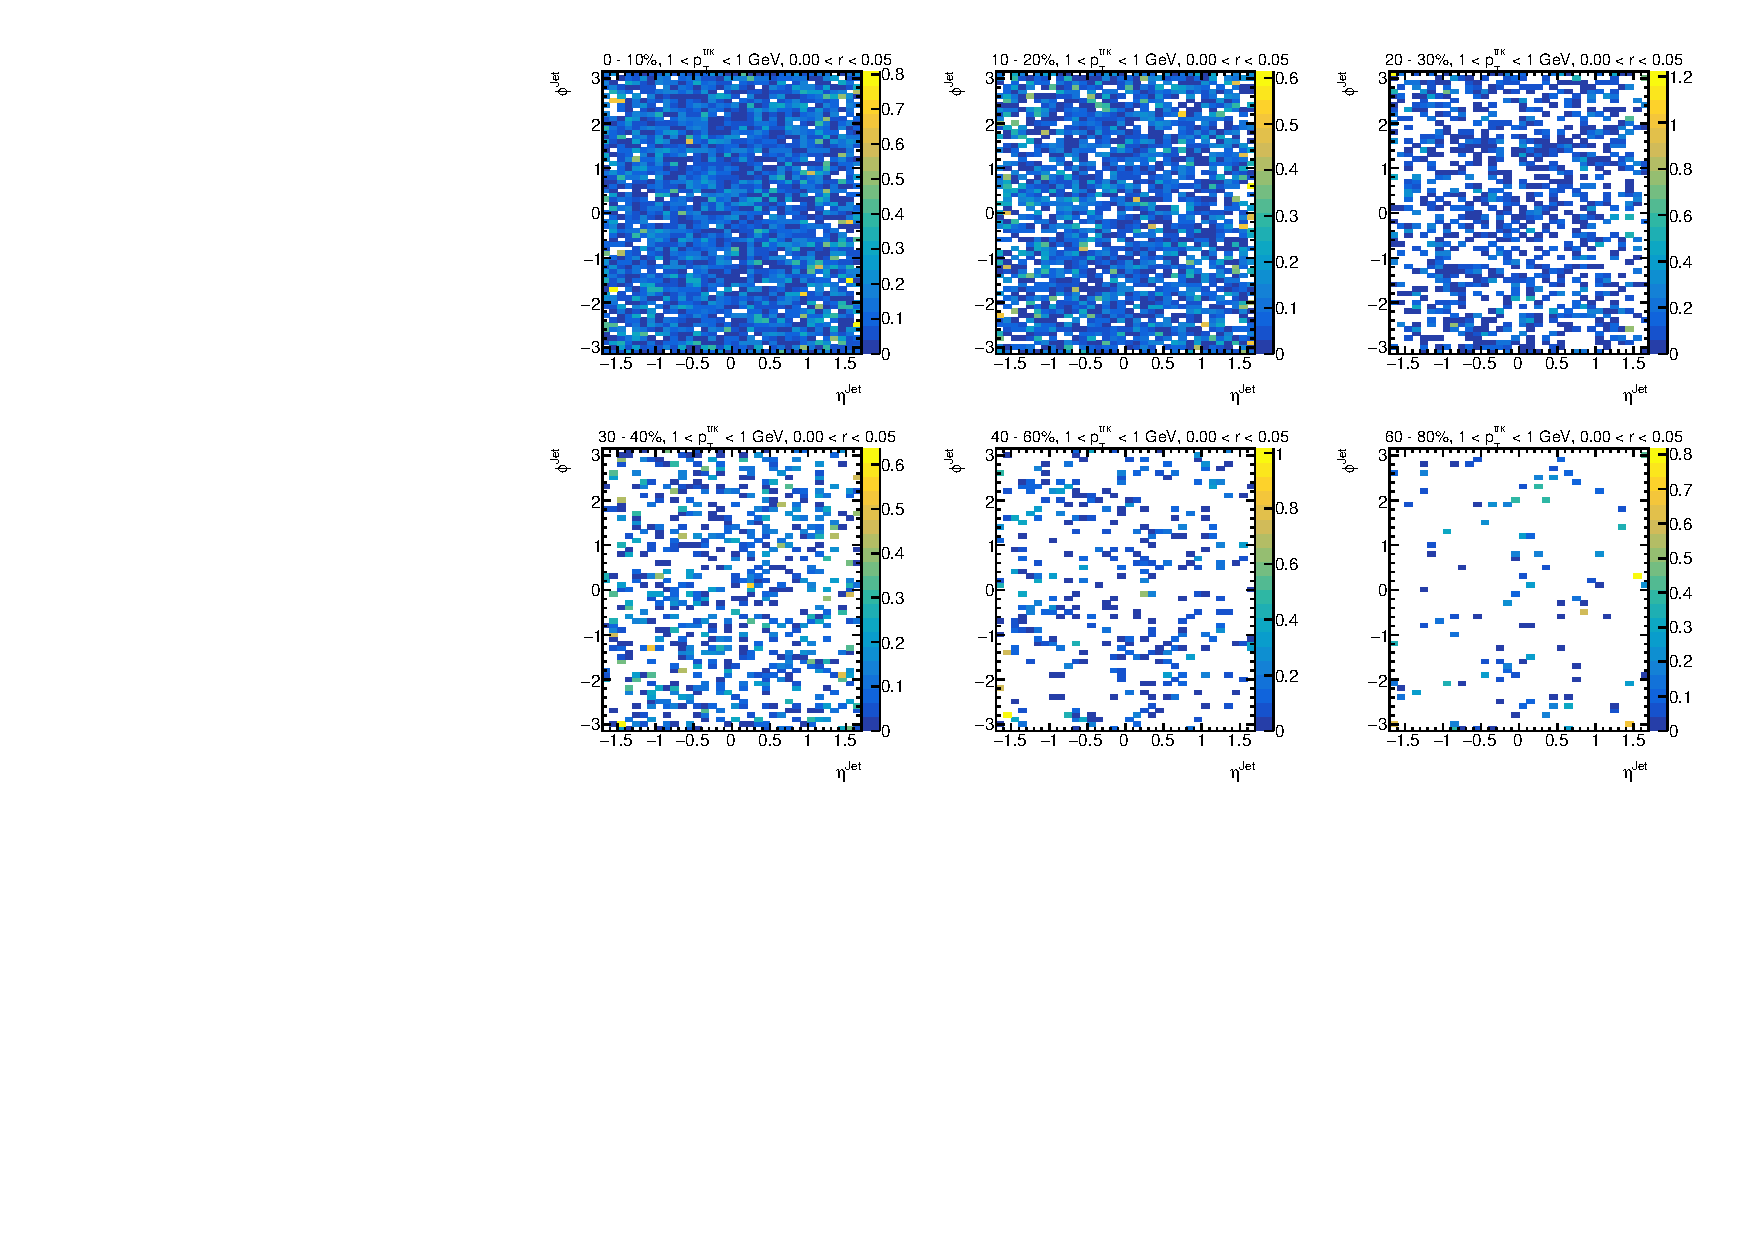
\includegraphics[width=1\textwidth]{figures/main/UE/eta_phi_map_trk2_dR0}
\caption{}
\end{subfigure} \quad
\begin{subfigure}{.5\textwidth}
\centering 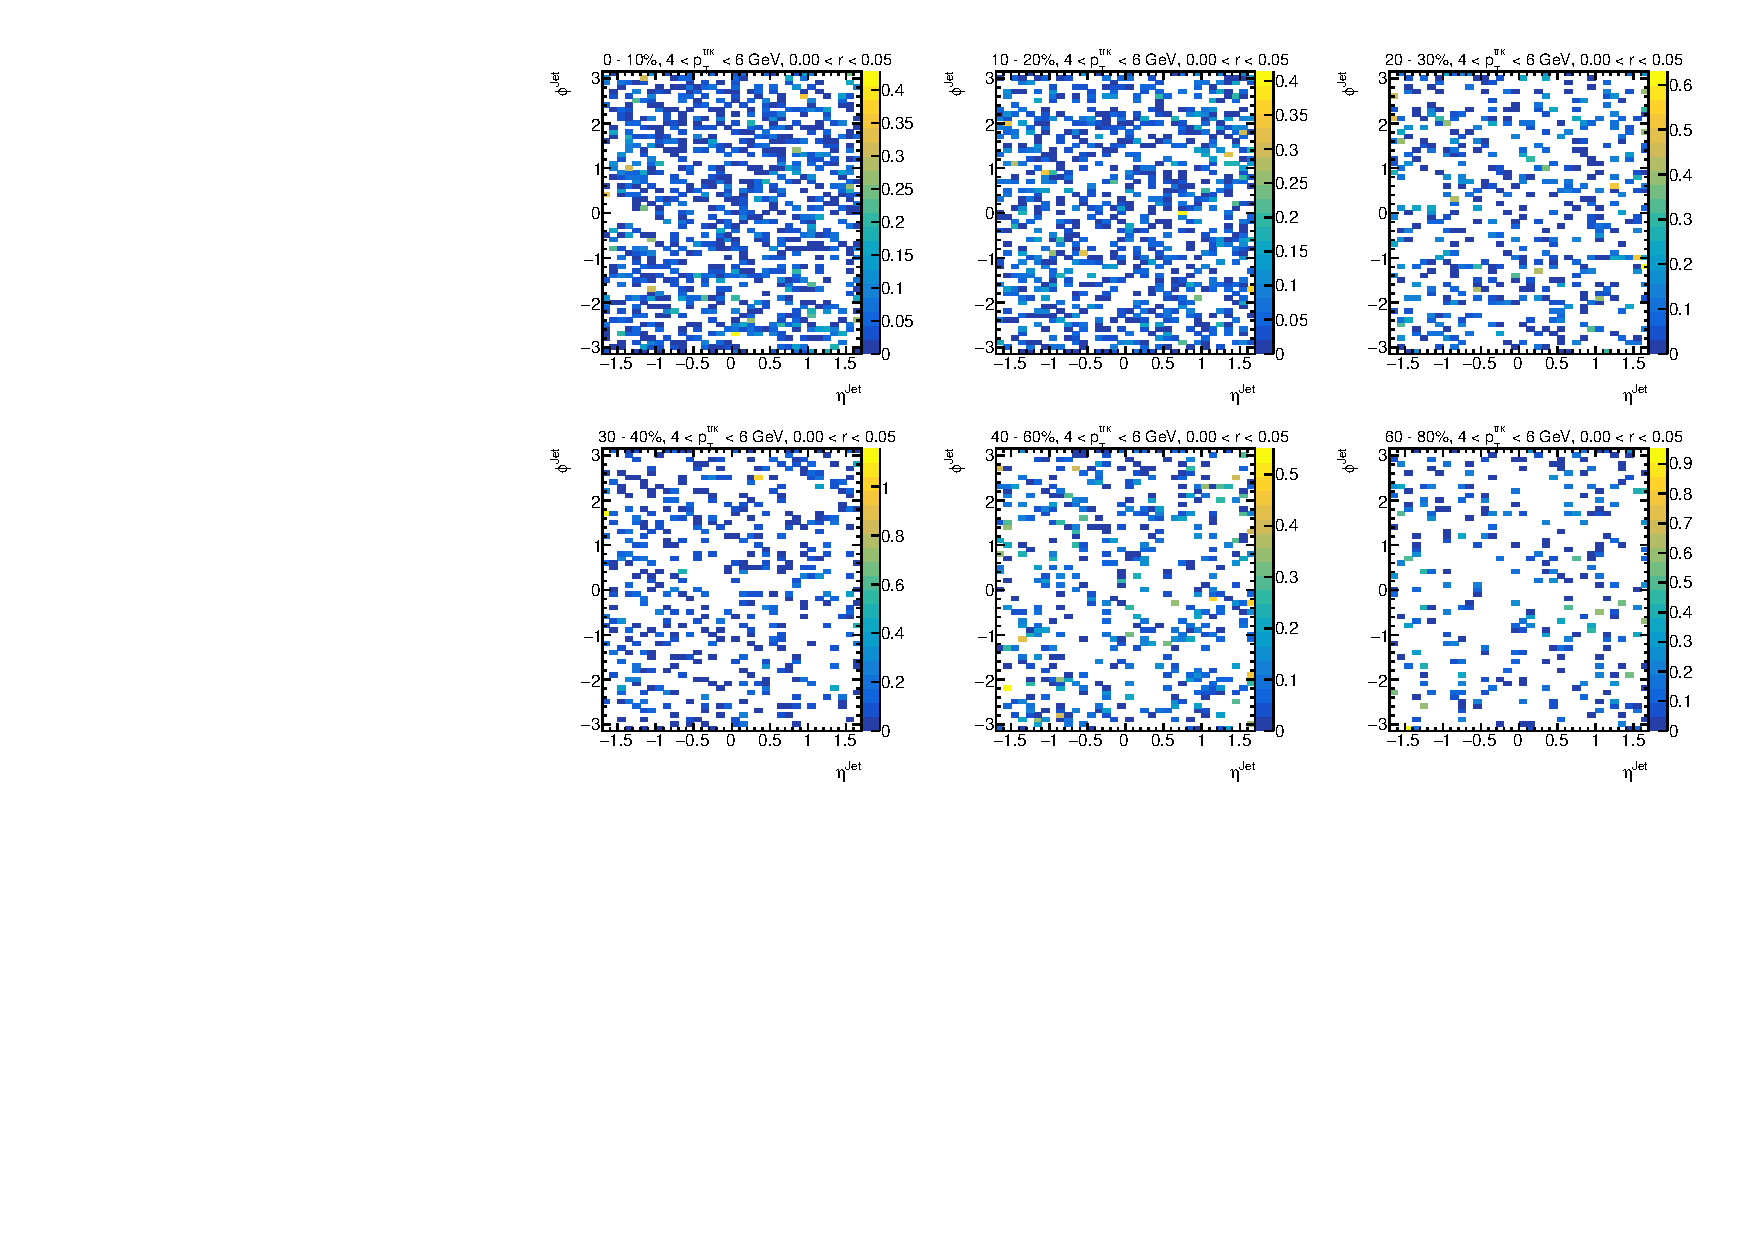
\includegraphics[width=1\textwidth]{figures/main/UE/eta_phi_map_trk6_dR0}
\caption{}
\end{subfigure} \\
\begin{subfigure}{.5\textwidth}
\centering 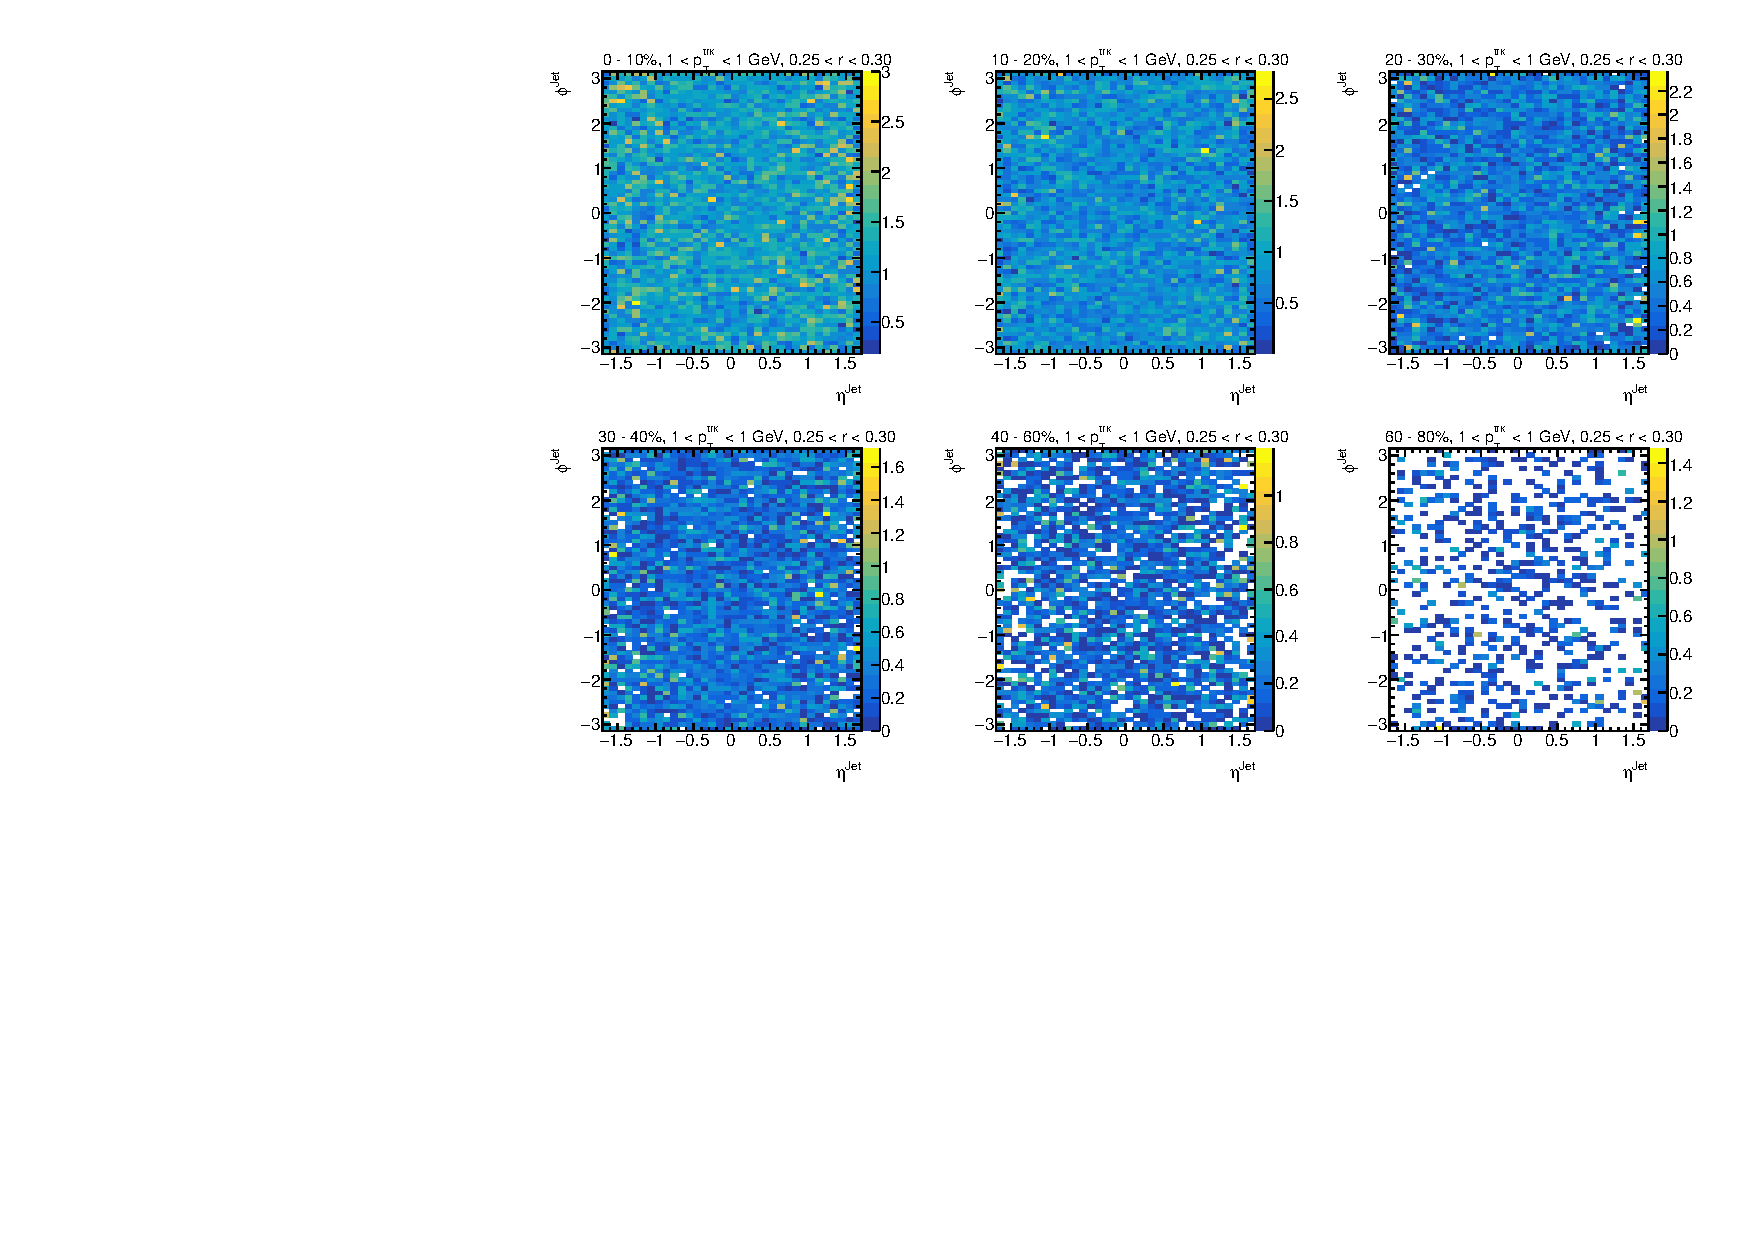
\includegraphics[width=1\textwidth]{figures/main/UE/eta_phi_map_trk2_dR5}
\caption{}
\end{subfigure}  \quad
\begin{subfigure}{.5\textwidth}
\centering 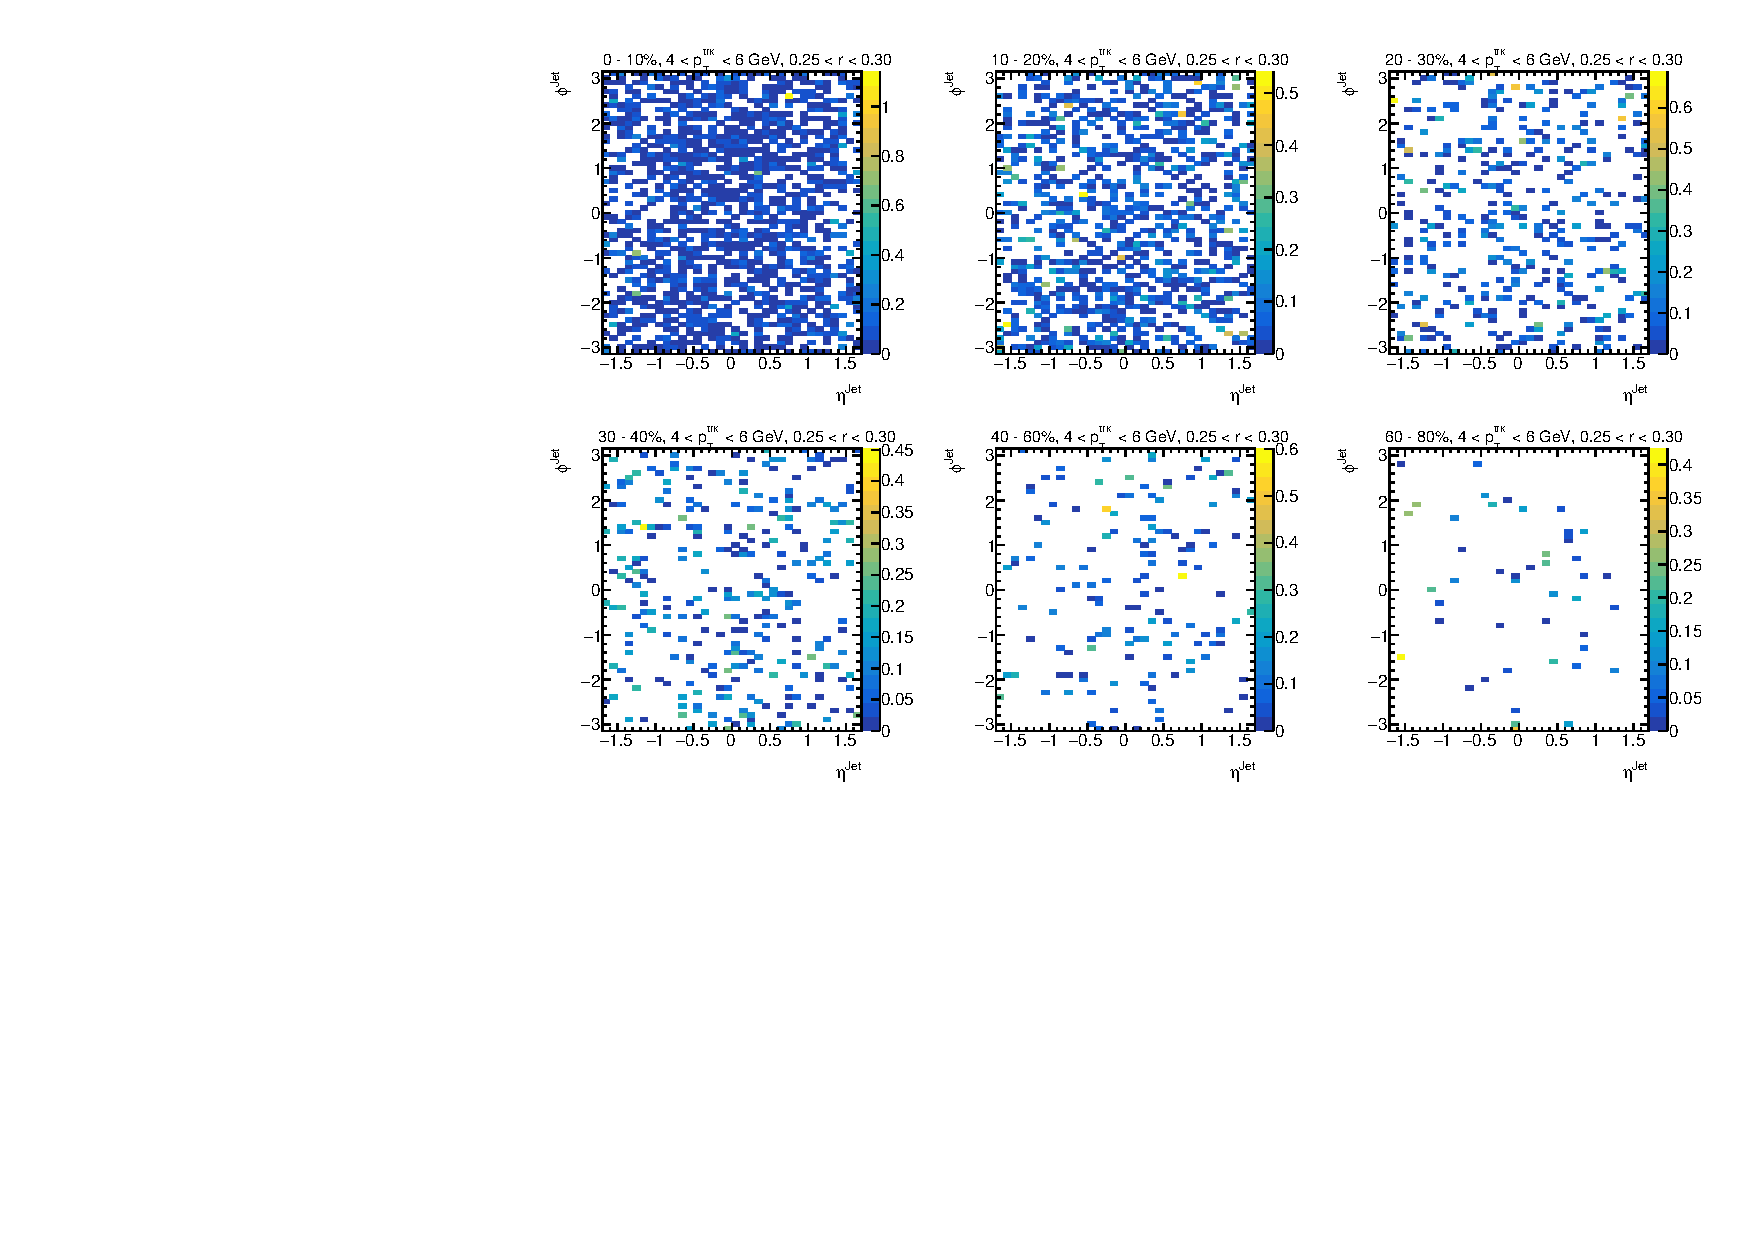
\includegraphics[width=1\textwidth]{figures/main/UE/eta_phi_map_trk6_dR5}
\caption{}
\end{subfigure} \\
\begin{subfigure}{.5\textwidth}
\centering 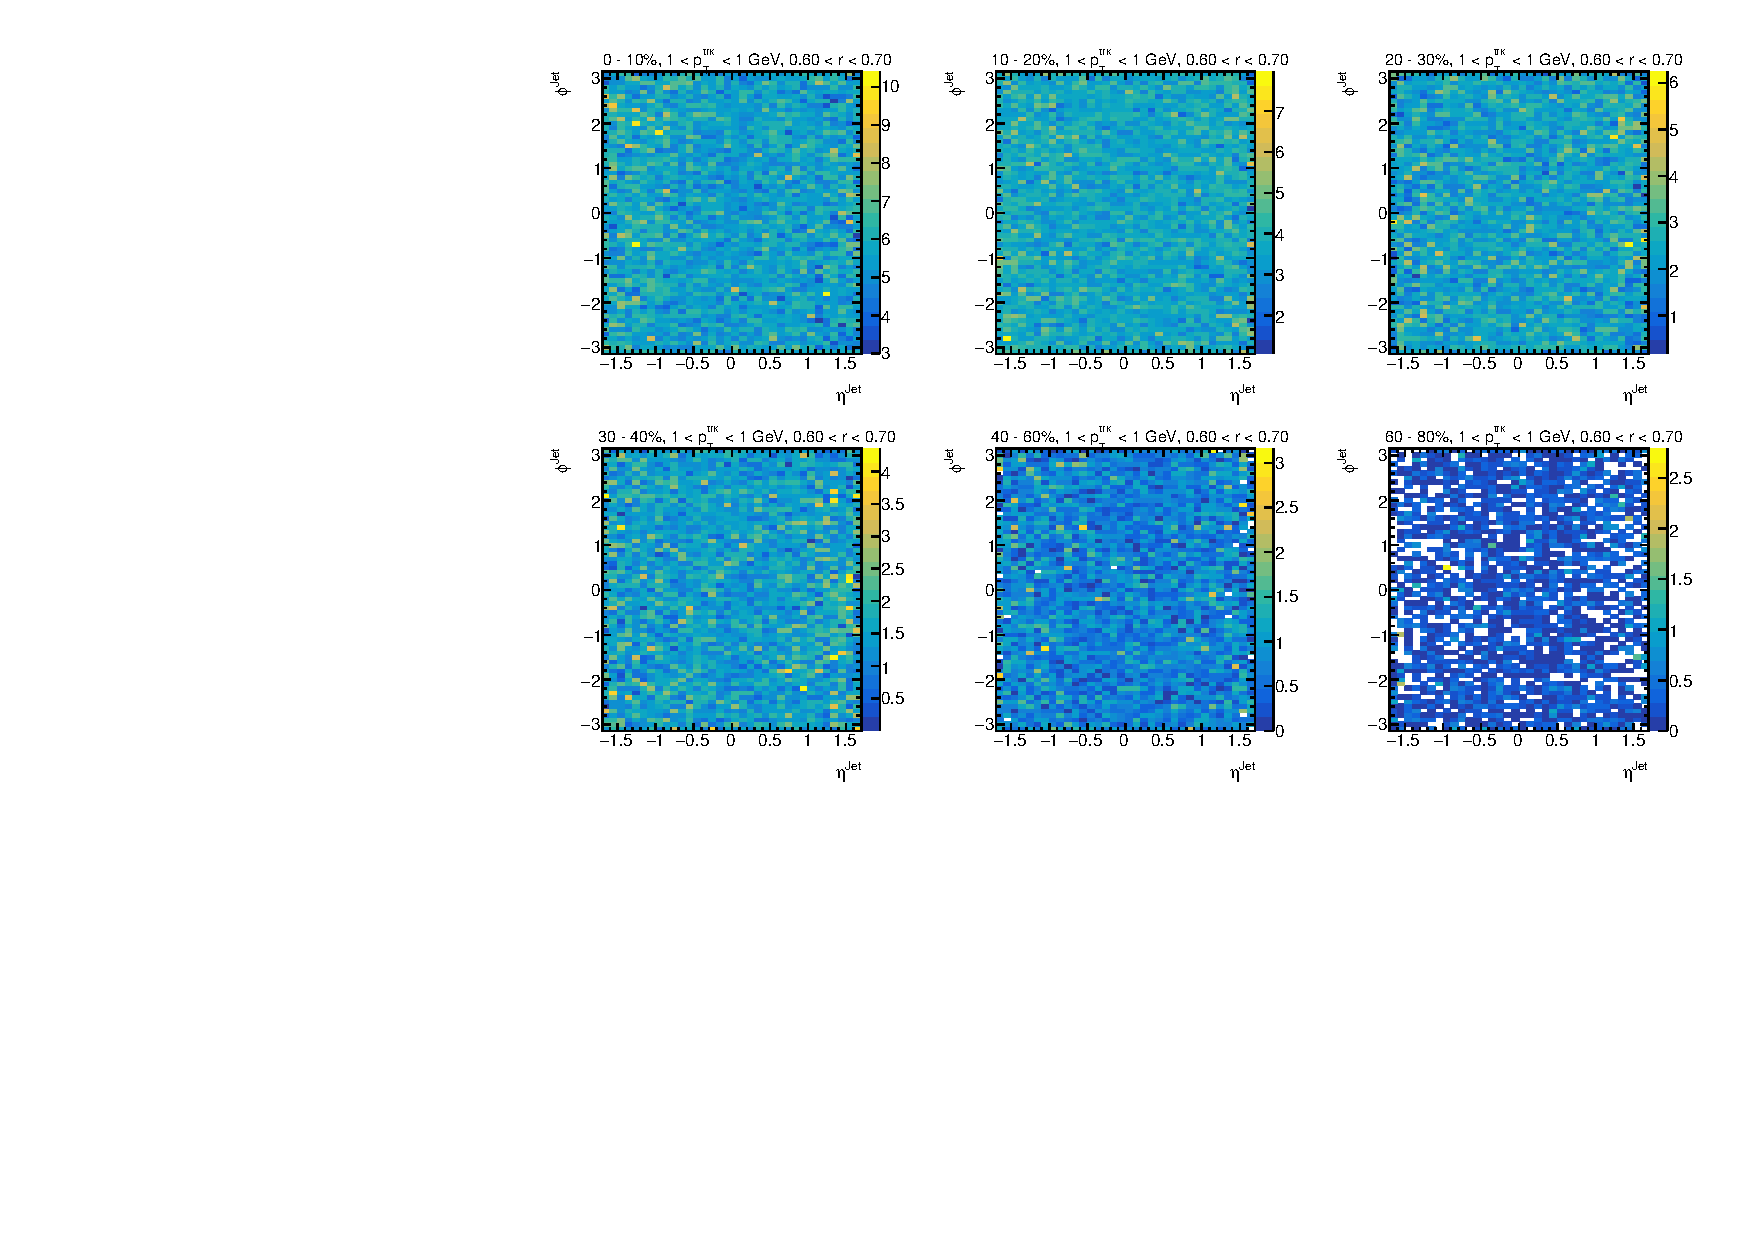
\includegraphics[width=1\textwidth]{figures/main/UE/eta_phi_map_trk2_dR9}
\caption{}
\end{subfigure} \quad
\begin{subfigure}{.5\textwidth}
\centering 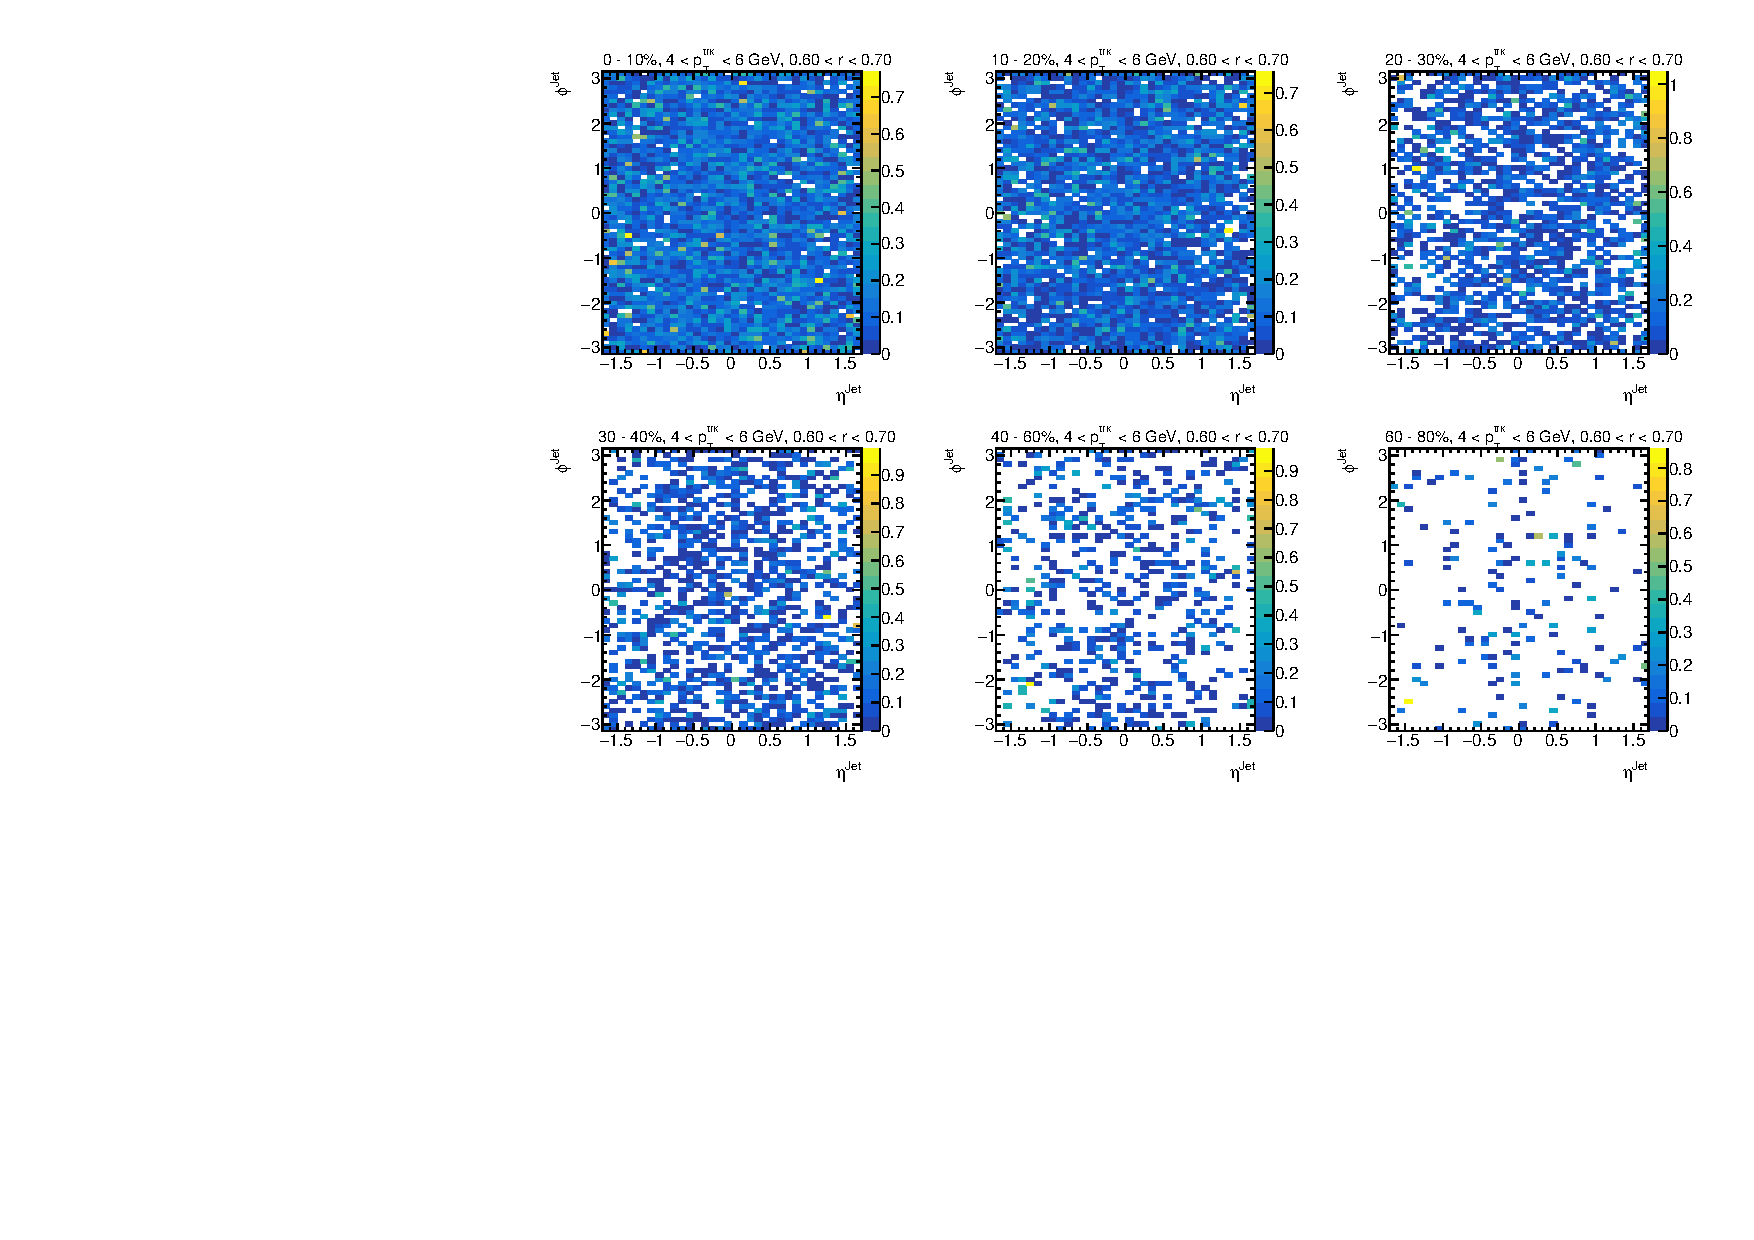
\includegraphics[width=1\textwidth]{figures/main/UE/eta_phi_map_trk6_dR9}
\caption{}
\end{subfigure}
\caption{Per jet $\nchUE^{\mathrm{Map}}$ distributions of charged particles evaluated for 1--1.6 GeV (left) and 4--6 GeV tracks in the jet core (top), near the jet edge (middle), and far from the jet (bottom) for  $\mathrm{d}\Psi$ in the interval 0.8--1.00, for six centralities, and 126--158 GeV jets.}
\label{fig:ue_map}
\end{figure}


The underlying event is then estimated by convoluting the $\nchUE^{\mathrm{Map}}$ distributions with the $\eta_{\mathrm{jet}}$, $\phi_{\mathrm{jet}}$, and $\mathrm{d}\Psi_{\mathrm{jet}}$ distributions of jets.
The UE estimated by this method in MC consists of tracks without a truth match, and hence is the ``true'' underlying event by definition.
This $\mathrm{UE}^{\mathrm{MC}}$ can then be used to correct any correlations between the underlying event as determined by the cone method and the JER (discussed in later sections).
The UE normalized to unit area, as a function of $\Delta R$ with respect to the jet axis is shown in Figure~\ref{fig:UEdR} for the lowest track \pt\ interval where the UE contribution is the largest.
The two distributions are the UE with and without secondary particles.
The UE strongly decreases for more peripheral collisions and for increasing track \pt.
Little radial dependence is seen when the secondaries are not included.
A small effect is expected because there is an enhancement in the number of jets at mid rapidity, along with a decrease in the UE yield as a function of $\eta$.
Since the secondaries are generated by primary PYTHIA particles, the enhancement is expected towards the jet core, where there is a higher multiplicity of primary particles.

%The map method is then applied to data to measure the UE charged particle contribution to the measured \Dptr\ distributions.
%Since this method uses real MB \pbpb\ collisions (from the MC overlay samples that have been reweighed to match the centrality distribution in data), the underlying event distribution is the same as in the data.
%This method does not require a correction for the correlation between the underlying event and the JER because it is based on tracks without a truth match.

\begin{figure}
\centering
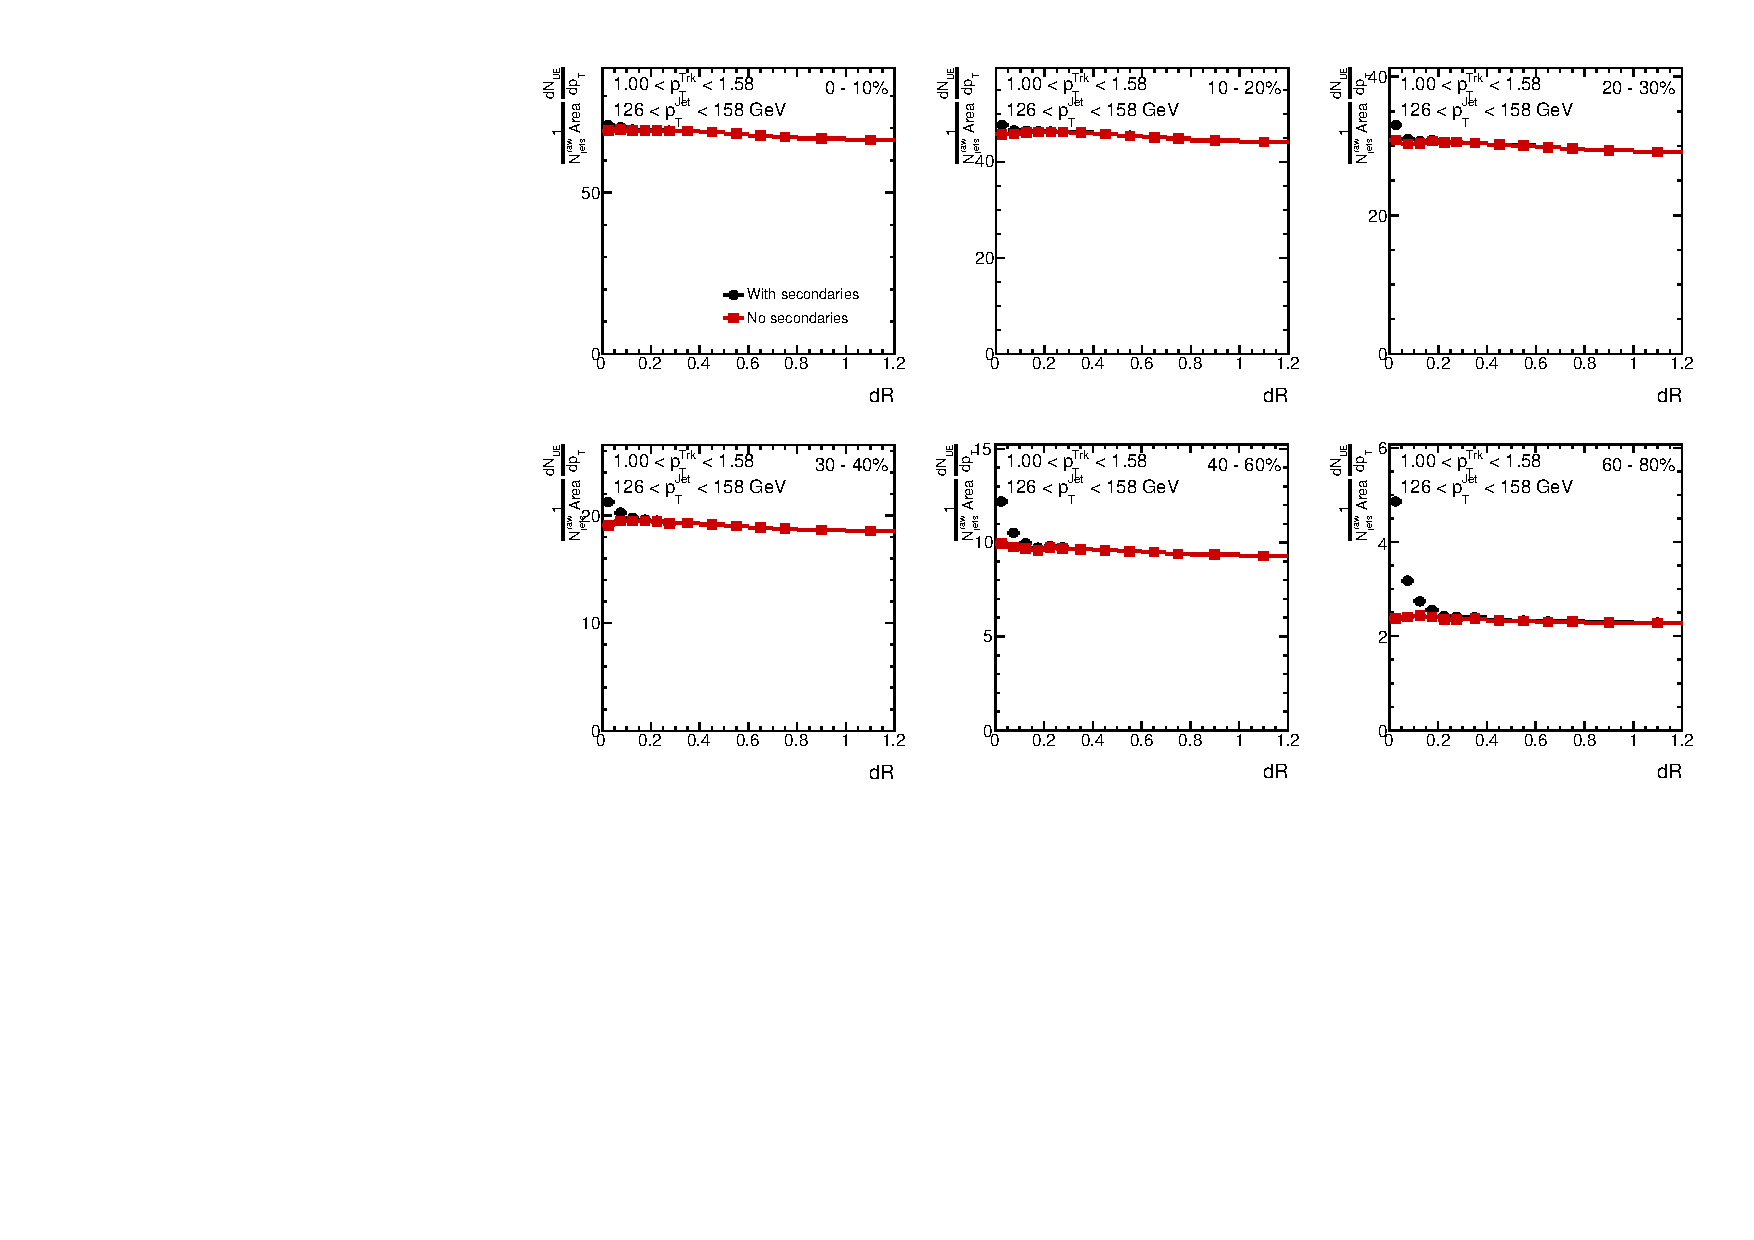
\includegraphics[width=0.9\textwidth]{figures/main/UE/UE_v_dR_pt1GeV.pdf}
\caption{UE estimated from tracks which do not have an associated truth particle in jet with \pt\ from 126 to 158 GeV and for the lowest track \pt\ interval (1--1.58 GeV).
The two different distribution shows the UE with and without the contribution from the secondary particles.}
\label{fig:UEdR}
\end{figure}   

%%%%%%%%%%%%%%%
\subsubsection{Cone Method}
\label{sec:cone_method}
The cone method uses a regular grid of 9 cones of size $R = 0.8$ covering the full inner detector region (shown in Figure~\ref{fig:cone_grid}).
The size of the cone corresponds to the radial phase space being investigated (0.8 in this case).
Cones within a distance of $dR=1.6$ to a reconstructed jet are excluded if $\ptjet > 90$ GeV.
They are also excluded if they contain a track with $\pt > 10$ GeV.
The 10 GeV was cut was chosen based on the small centrality dependence of the combined rate of fake and underlying event tracks above 10 GeV as shown in Figure~\ref{fig:fakeratehijing}.
The fraction of events as a function of number of cones used in each centrality bin is shown in Figure~\ref{fig:cone_stats}.
It can be seen that in the MC the number of cones used is consistent with there being no jet quenching.
This is as expected since the jets in the \pbpb\ MC overlay are coming from \pythia\ and are unquenched.
Moreover, quenching in central \pbpb\ data leads to only one jet causing exclusions, consistent with most events using 7 cones.
For more peripheral \pbpb\ collisions, the cone distribution tends to look like the distribution with no quenching.

\begin{figure}
\centering
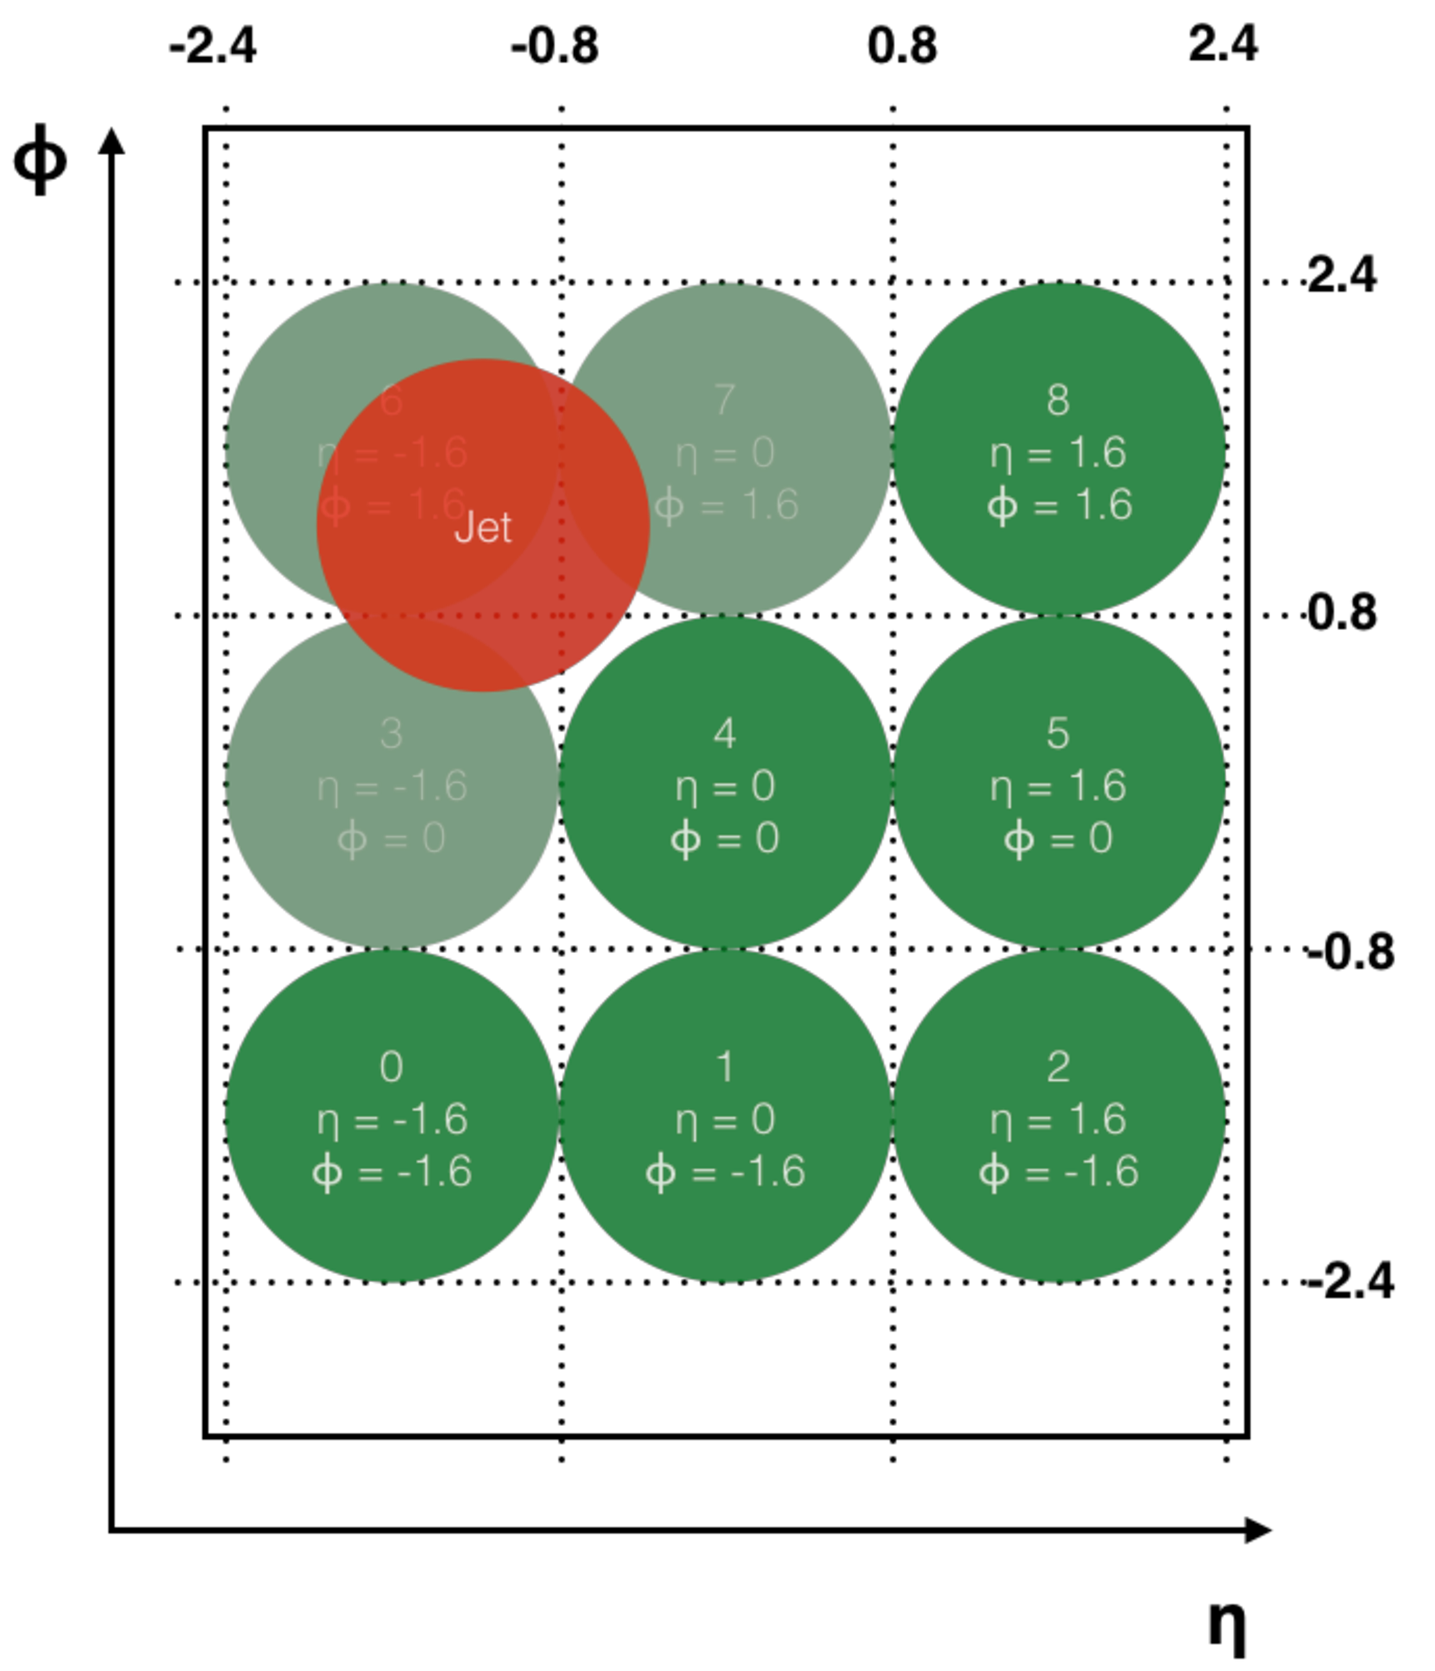
\includegraphics[width=0.45\textwidth]{figures/main/UE/cone_grid.pdf}
\caption{Illustration of the cone method to estimate the underlying event.
Cones numbered 3, 6, and 7 are excluded based based on the jet shown in red.}
\label{fig:cone_grid}
\end{figure}   

\begin{figure}
\centering
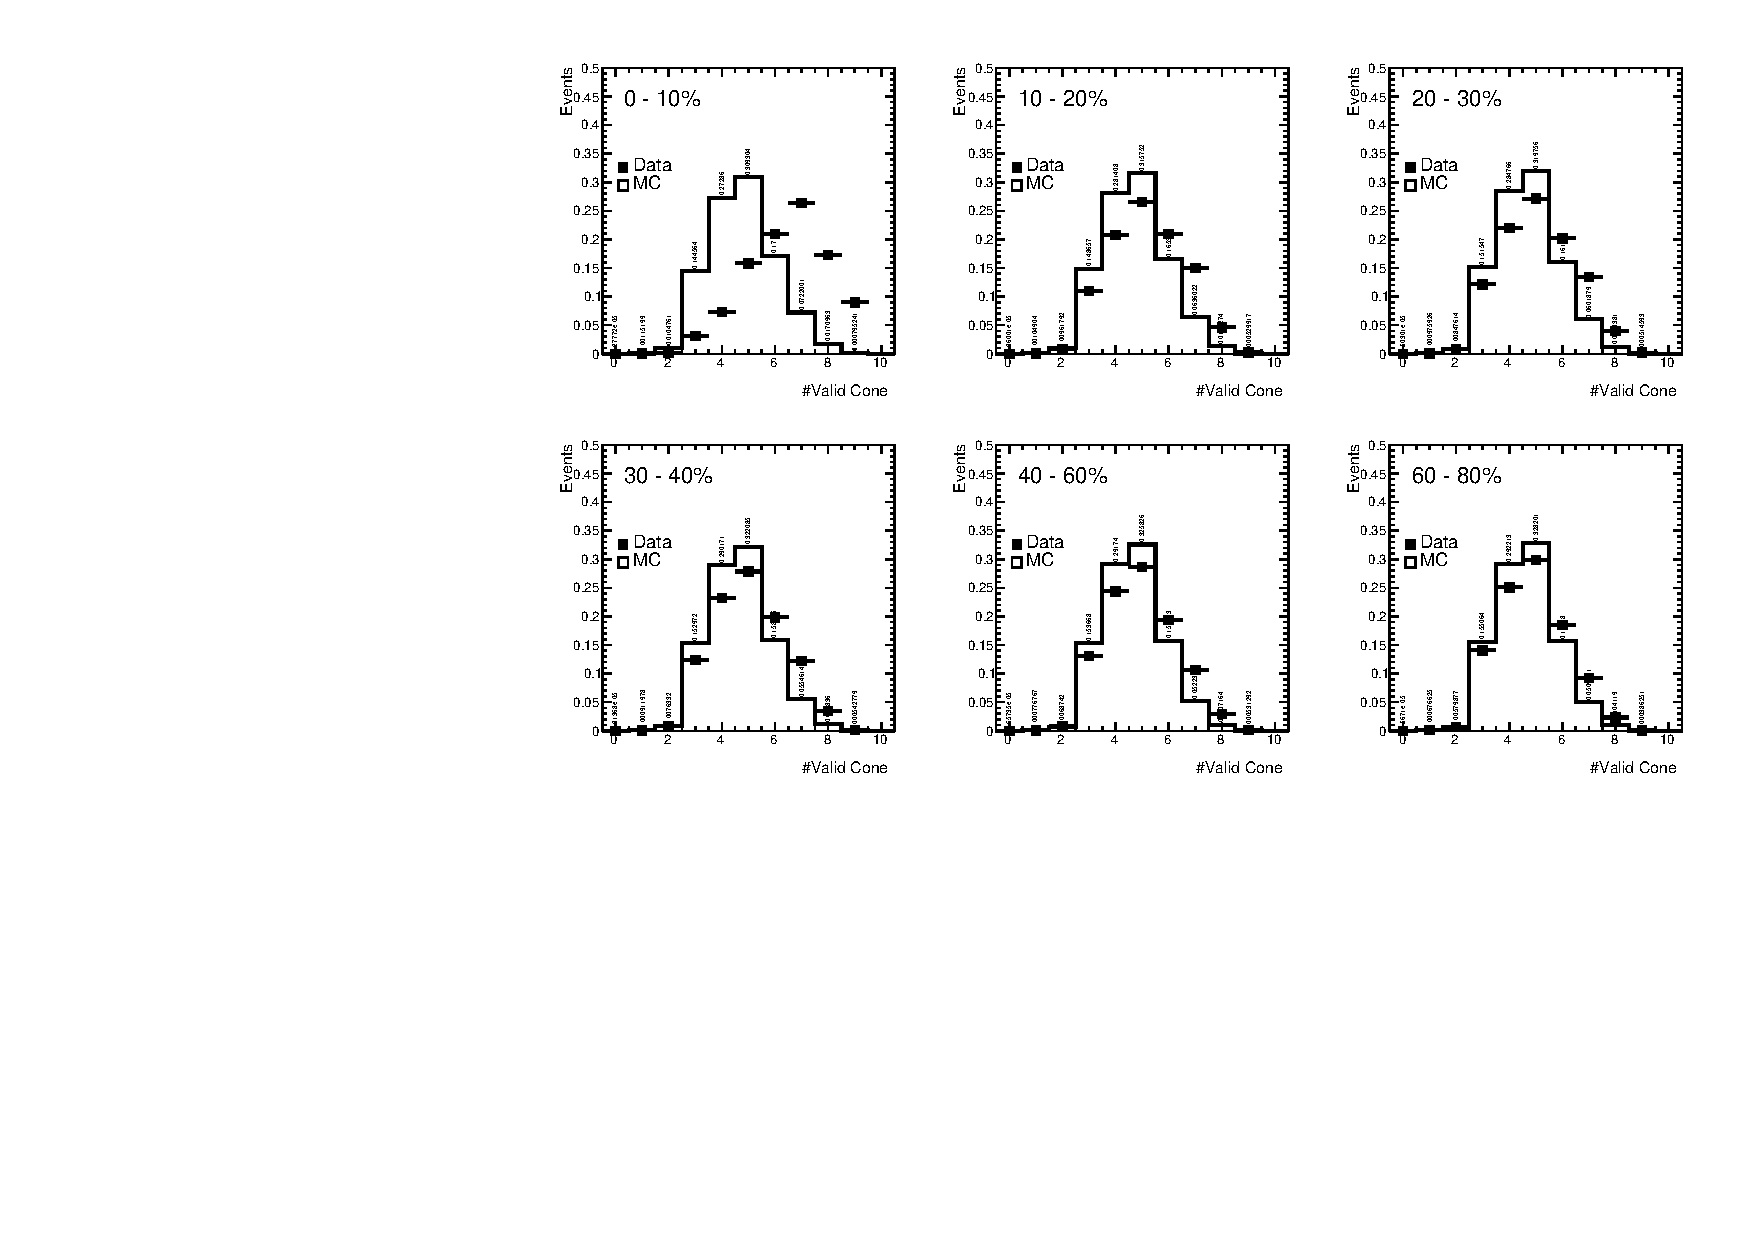
\includegraphics[width=0.9\textwidth]{figures/main/UE/cone_stats}
\caption{Fraction of events as a function of the number of cones used for the estimation of the underlying event.}
\label{fig:cone_stats}
\end{figure}   

The resulting UE charged particle yields $\fd \nchUE^{\mathrm{Cone}}/ \fd \pTch$ are evaluated over the 1 -- 10 GeV range as a function of \pt\, \ptjet\, centrality, and \rvar, and then averaged over all cones according to.

\begin{eqnarray}
\frac{\fd n_{\mathrm{ch}}^{\mathrm{UE Cone}}}{\fd \pTch}  = \frac{1}{N_{\mathrm{cones}}} \frac{1}{\varepsilon} \frac{\Delta N^{\mathrm{cone}}_{\mathrm{ch}} (\pTch, \ptjet, \etajet)}{\Delta \pTch}
\end{eqnarray}
Here $N_{\mathrm{cones}}$ is the number of background cones associated with a given jet with \ptjet.
$\Delta N^{\mathrm{cone}}_{\mathrm{ch}}$ is the number of charged particles summed across all background cones associated to the jet in question.
The cone method estimates the UE yields only from events containing jets included in the analysis, ensuring that the background automatically had the correct distribution of centralities within a given centrality bin.

The UE contribution as measured using the cone method in data needs to be further corrected for three effects:

\paragraph{Correction for $\eta$-dependence:}
To account for differences in the yields of UE particles at the position of the jet and at the position of the track for the random cone entering the UE estimate, the $\eta$ distribution of charged particles from MC overlay events is used to appropriately weigh the UE tracks.
The correction is then the ratio of the value of the $\fd \nch / \fd\eta$ at the position of the jet and the track.
The impact of the correction in 0-10\% \pbpb\ collisions is shown in Figure~\ref{fig:eta_corr}

%\begin{figure}
%\centering
%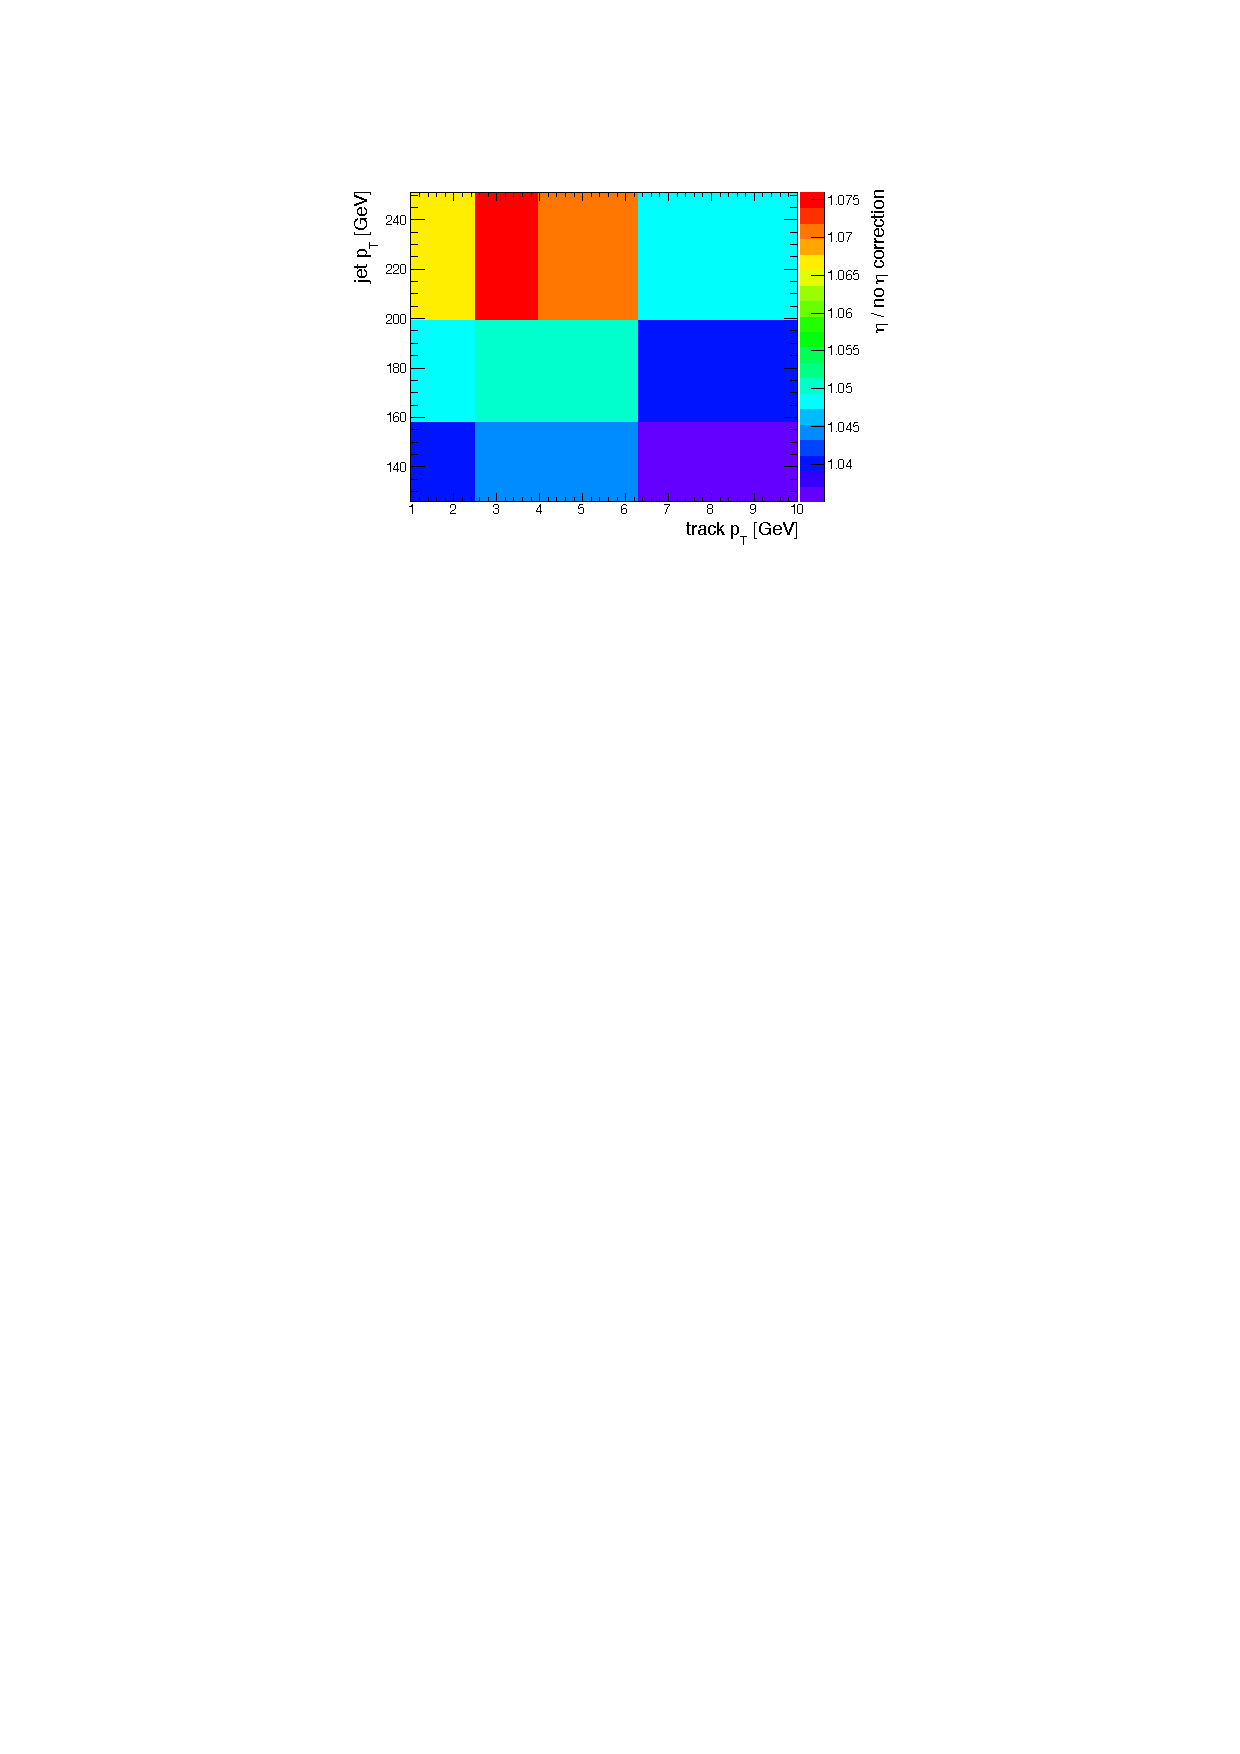
\includegraphics[width=0.45\textwidth]{figures/main/UE/eta_correction.pdf}
%\caption{Ratio of the $\NchUECone$ distributions with and without the correction for $\eta$ dependence in the most central 0-10\% \pbpb\ collisions, evaluated with a subset of the data (70k events).
%Figure from Ref.~\cite{Sickles:2235420}.}
%\label{fig:eta_corr}
%\end{figure}


\paragraph{Correction for flow:}
Elliptic flow is the characteristic sinusoidal modulation of the yields of particles along the azimuth in heavy ion collisions.
The maximum amplitude of the modulation determines the reaction plane, with more momenta being measured in plane than out of plane.
Ref.~\cite{Aaboud:2018ves} provides a basic measurement of the magnitude of the elliptic flow, and its \pt\ dependence.
The correction for this effect was based on a parametrization of the \pTch and centrality dependence of previously measured elliptic flow coefficients, $v_{2}$ \cite{Aaboud:2018ves}.
The reaction plane angle $\Psi$ is estimated on an event-by-event basis by using the $\phi$ variation of transverse energy in the forward calorimeter.
The correction factor is evaluated as a function of the distance of the jet from the reaction plane $\cos2(\phijet - \Psi)$.
The correction is less (greater) than unity for jets in a direction perpendicular (parallel) to the reaction plane.
Jets perpendicular (parallel) to the plane typically have a lower (higher) UE, and a cone at a random position in the ID is corrected down (up).
The size of the correction is at the level of a few percent, and decreases with increasing track \pt, as is shown in Figure~\ref{fig:flow_corr}


\begin{figure}
\begin{subfigure}{0.5\textwidth}
\centering 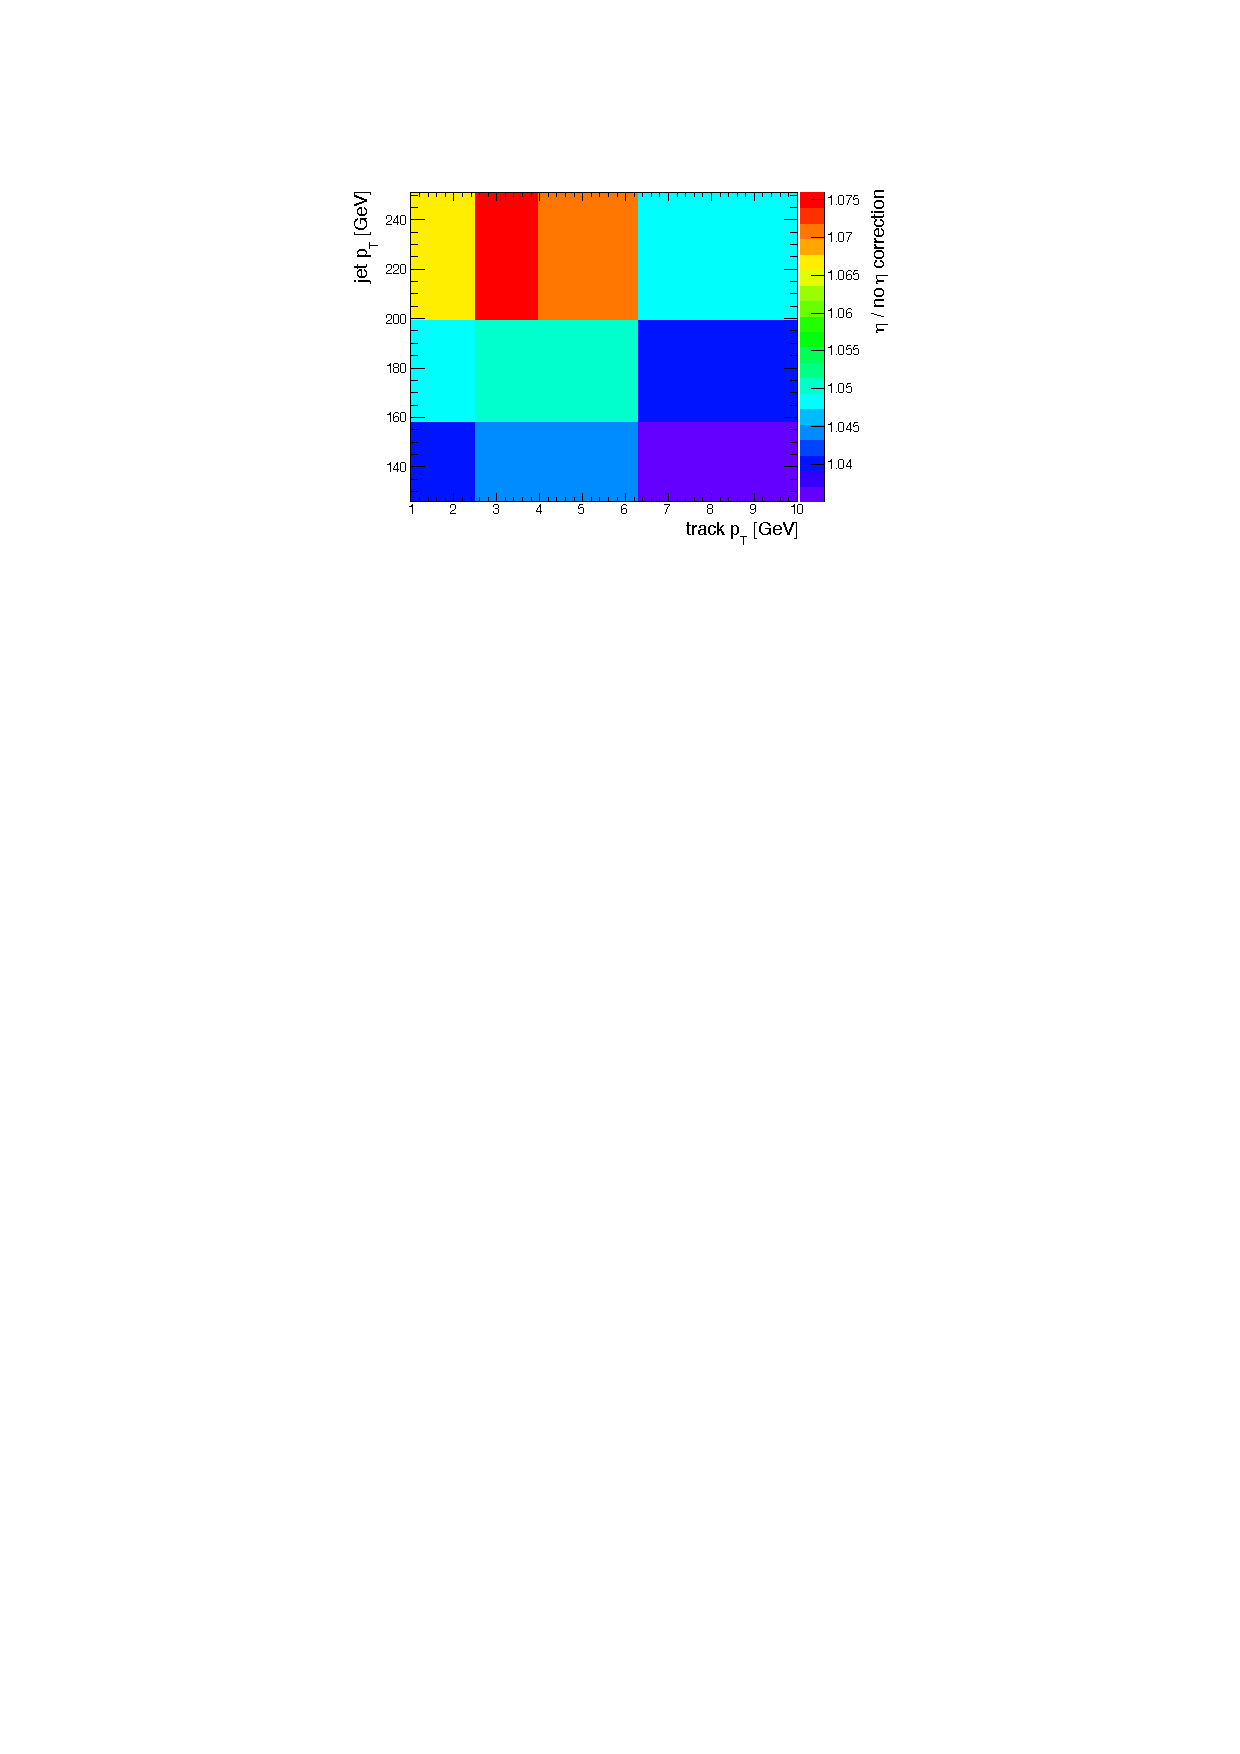
\includegraphics[width=1\textwidth]{figures/main/UE/eta_correction.pdf}
\caption{}
\label{fig:eta_corr}
\end{subfigure}
\begin{subfigure}{0.5\textwidth}
\centering 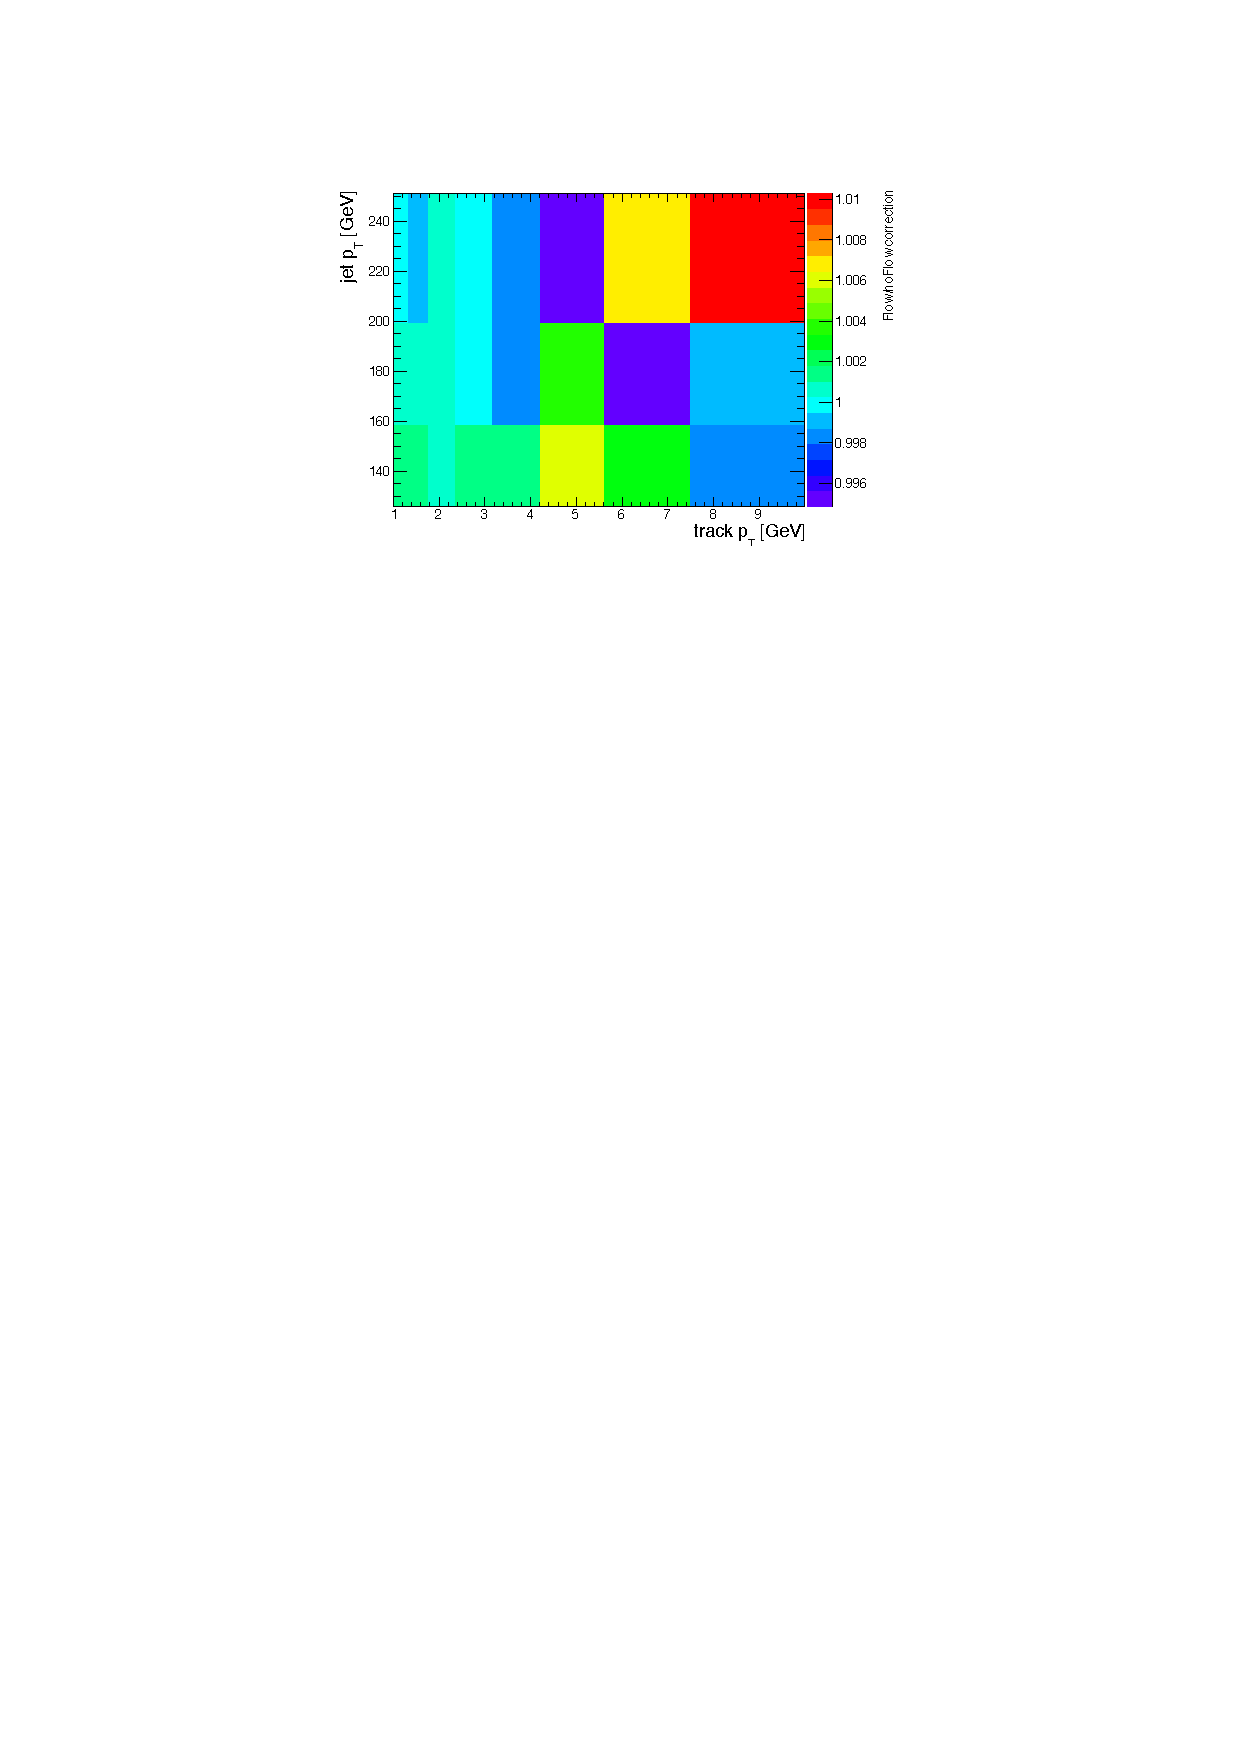
\includegraphics[width=1\textwidth]{figures/main/UE/flow_correction.pdf}
\caption{}
\label{fig:flow_corr}
\end{subfigure}
\caption{Ratio of the $\NchUECone$ distributions with and without the correction for (left) $\eta$ dependence and (right) elliptic flow in the most central 0-10\% \pbpb\ collisions, evaluated with a subset of the data (70k events).
Figures from Ref.~\cite{Sickles:2235420}.}
\label{fig:cone_corrections}
\end{figure}



%\begin{figure}
%\centering
%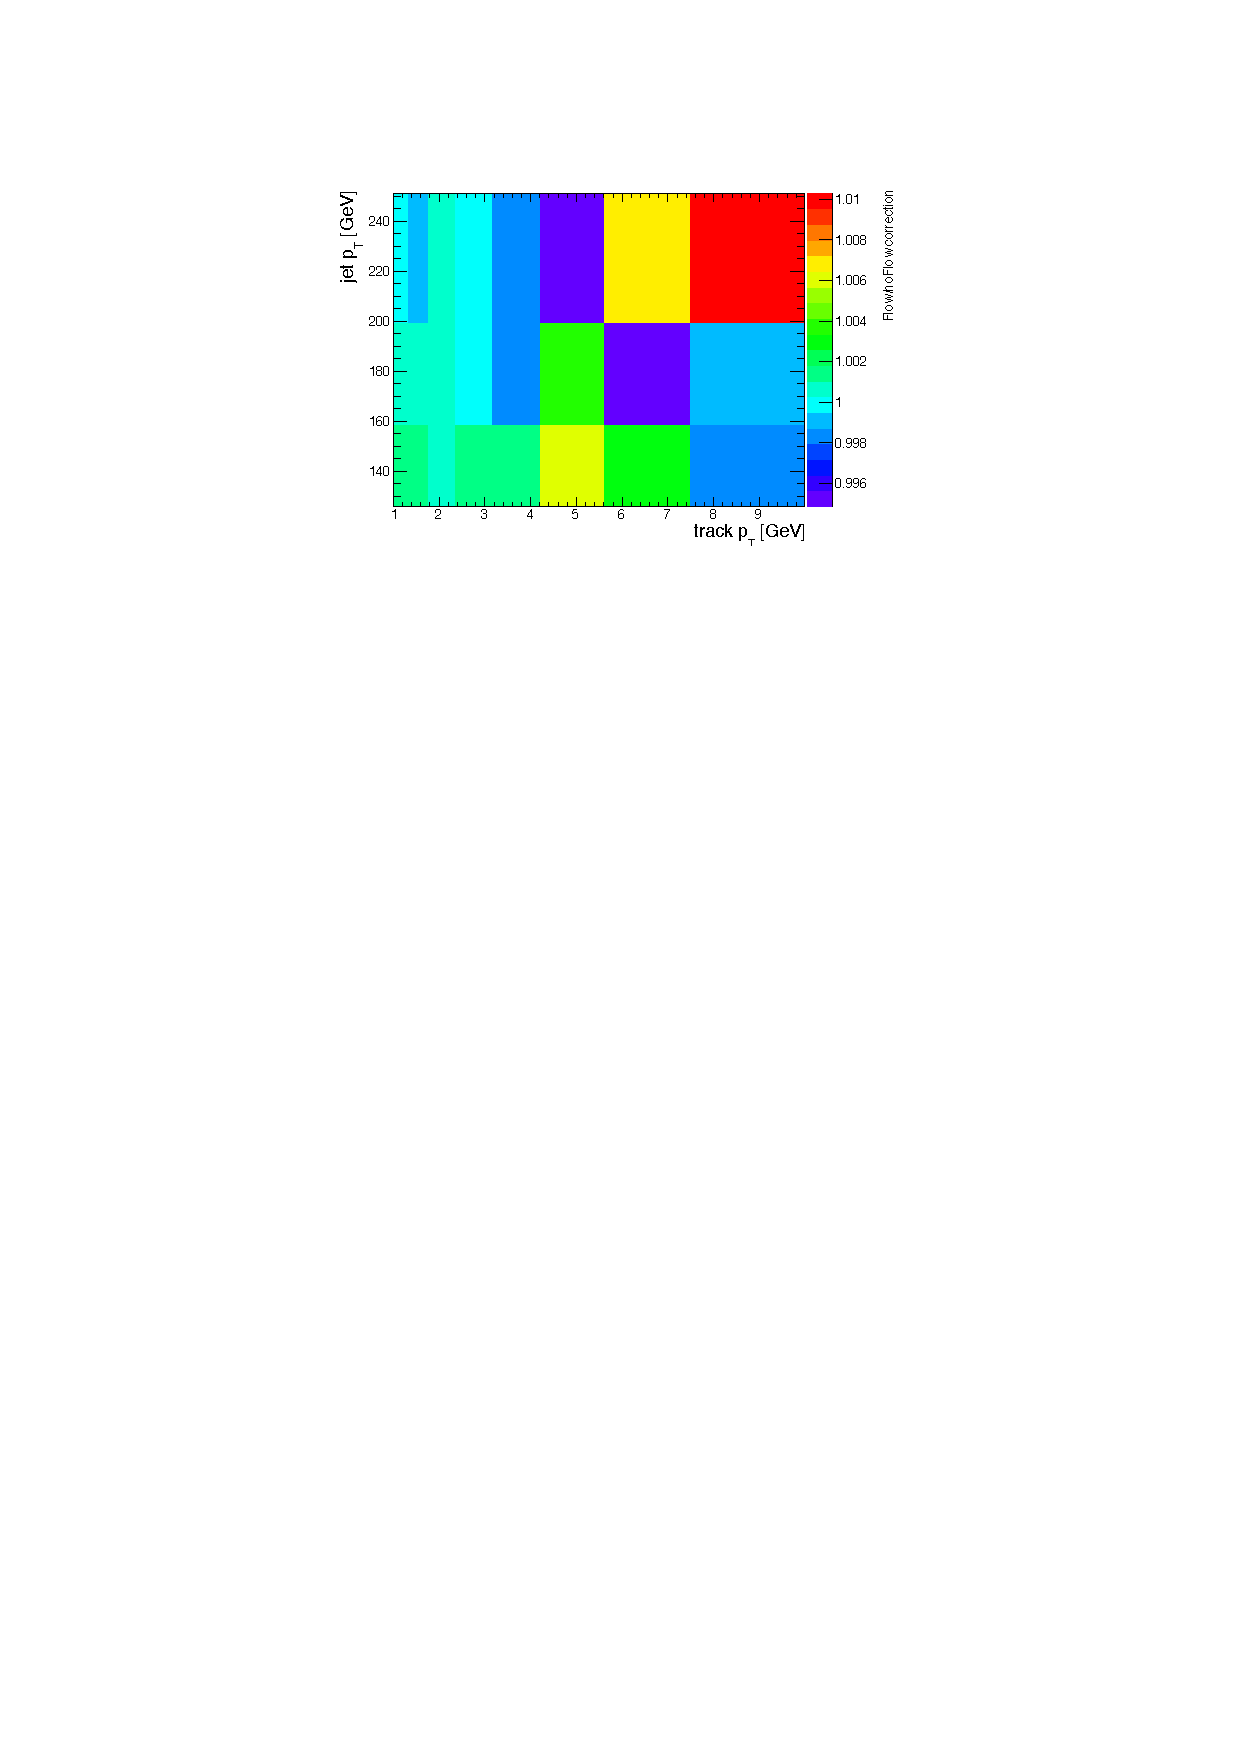
\includegraphics[width=0.45 \textwidth]{figures/main/UE/flow_correction.pdf}
%\caption{Ratio of the $\NchUECone$ distributions with and without the correction for elliptic flow in the most central 0-10\% \pbpb\ collisions, evaluated with a subset of the data (70k events).
%Figure from Ref.~\cite{Sickles:2235420}.}
%\label{fig:flow_corr}
%\end{figure}

\paragraph{UE and JER correlation:}
The interplay between the UE and the JER will be described here is discussed in further detail in Ref.~\cite{ATLAS-COM-PHYS-2012-1653}.
Due to the steeply falling nature of the jet \pt\ spectra, the smearing due to jet energy resolution leads to a net migration of jets from lower \pt\ to higher \pt\ values (hereafter referred to as ``up-feeding'') such that a jet reconstructed with a given \pTrec\ will correspond, on average, to a lower truth jet \pT, \avgpttrue.
The up-feeding was observed to induce in the MC a difference between the UE yields determined using the MC overlay events and the actual UE contribution to reconstructed jets.
The magnitude of this difference was found to be centrality dependent and exhibited a weak \pTjet\ dependence.
That difference was found to result from intrinsic correlations between the UE contribution to the yield of particles measured inside the jet and the MC \pTjet\ shift, $\Delta p_{\mathrm{T}}^{\mathrm{jet}}= \pTrec - \pTtrue$.
In particular, jets with positive (negative) $\Delta p_{\mathrm{T}}^{\mathrm{jet}}$ were found to have an UE contribution larger (smaller) than jets with $\Delta p_{\mathrm{T}}^{\mathrm{jet}} \sim 0$.

To correct for this effect, the centrality-, $\pTjet$-, $r-$ and $\pTch$-dependent multiplicative correction factors were applied on $\fd \nchUE^{\mathrm{Cone}}/ \fd \pTch$ distributions.
These multiplicative factors, $w_{\mathrm{UE}}$, were estimated as a ratio of UE distributions calculated in MC samples using the "Map method", $\Dptr_{f}$, and the "Cone Method".

\begin{eqnarray}
w_{\mathrm{UE}} (\pT) = \frac{\fd \nchUE^{\mathrm{Map}}/ \fd \pTch}{\fd \nchUE^{\mathrm{Cone}}/ \fd \pTch}\bigg|_{\mathrm{MC}}
\end{eqnarray}   
Examples of these factors are shown in Figure~\ref{fig:UEweights}.
The correction by construction corrects also for fakes and secondary contribution in the track \pT\ region 1-10~GeV in \PbPb\ collisions.
%These factors are also shown in Figure~\ref{fig:UEweights_r_jet0}, as a function of \rvar\ for different track \pt\ bins, for $126 < \ptjet\ < 158 \GeV$.
The size of these corrections integrated over $\rvar = 0.4$ is comparable to the UE-JER correction done in \cite{PhysRevC.98.024908}.

\begin{figure}
\centering
\begin{subfigure}{1.\textwidth}
\centering \includegraphics[page=2,width=1.\textwidth]{figures/main/UE/UE_factors.pdf}
\caption{}
\label{fig:UEweights_r2}
\end{subfigure} \\
\begin{subfigure}{1.\textwidth}
\centering \includegraphics[page=6,width=1.\textwidth]{figures/main/UE/UE_factors.pdf}
\caption{}
\label{fig:UEweights_r6}
\end{subfigure}
\caption{The multiplicative correction factors that correct for the correlation between the UE and the JER, fake and secondary particles in different centrality classes and \mbox{$ 0.05 < r < 0.10$} (top) and \mbox{$ 0.25 < r < 0.30$ (bottom)}.}
\label{fig:UEweights}
\end{figure}

%\begin{figure}
%\centering
%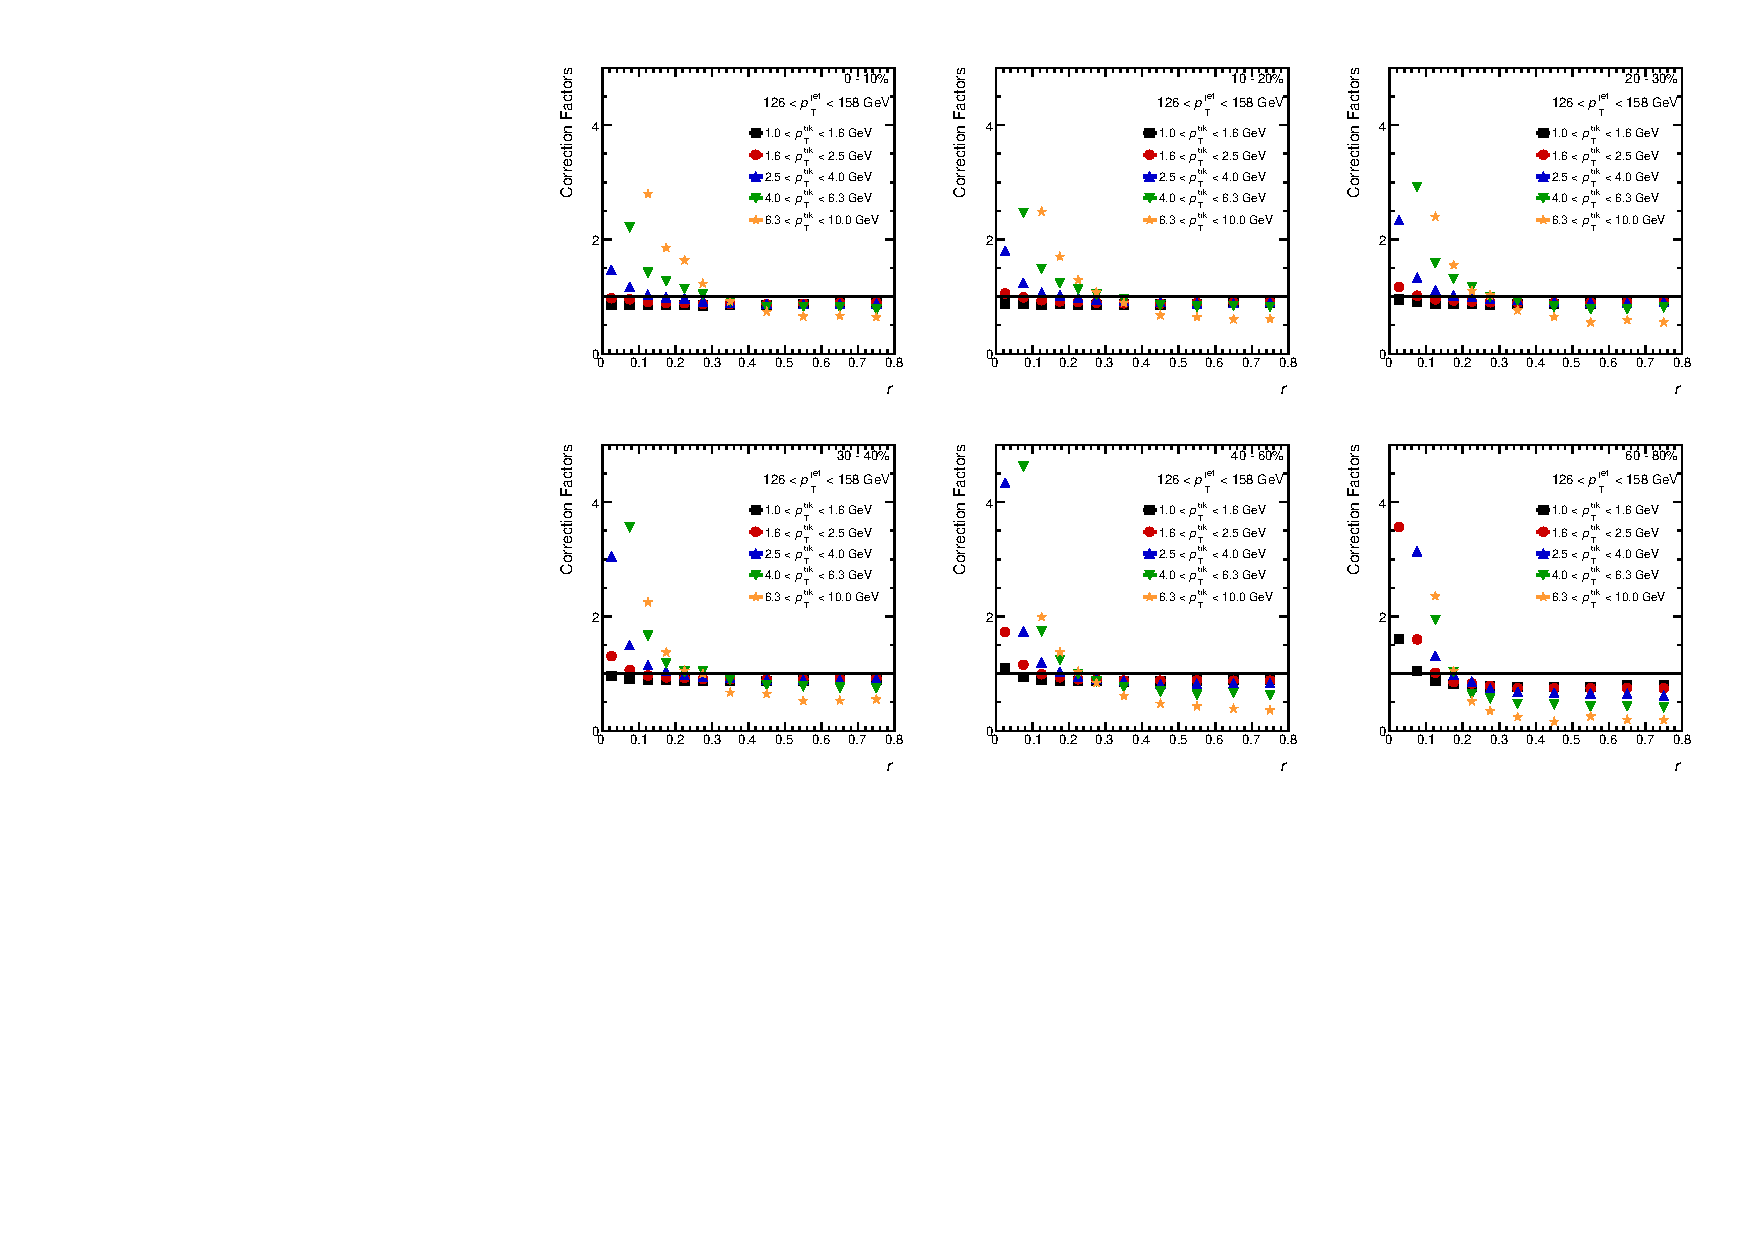
\includegraphics[page=1,width=1.\textwidth]{figures/main/UE/UE_factors_r.pdf} \\
%\caption{The multiplicative correction factors that correct for the correlation between the UE and the JER, fake and secondary particles in different centrality classes, as a function of $r$ for $126 < \ptjet < 158 \GeV$.}
%\label{fig:UEweights_r_jet0}
%\end{figure}


The absolute magnitude of the correction increases towards the higher track \pt\ in the jet core where the UE is smaller.
This behavior has two contributions: the intrinsic correlations between the UE contribution to the yield of particles measured inside the jet and the MC \pTjet\ shift as it was discussed earlier, and the correlation of production of secondary particles with the jet.
The production of secondary particles is associated with presence of primary particles.
Thus, the production of secondary particles is enhanced in the jet due to the higher density of primary particles compared to the regions outside a jet.
This was shown in Figure~\ref{fig:UEdR} where the UE evaluated in term of particles without matching to truth particles in MC with and without the contribution from secondary particles is presented and where the yield of secondary particles is significant only at smaller $dR$, that is, within a jet.
Figure~\ref{fig:UEdR} also shows that the relative yield of secondary particles to the yield of the UE particles is increasing with decreasing collisions centrality.
Furthermore, the relative contribution of secondary particles to the UE increases with the track \pT\ as the fraction of the secondary particles decreases only slowly with the increasing track \pT\ (Figure~\ref{fig:fakeratepbpb}), however, the UE decreases strongly with the increasing track \pT\ (Figure~\ref{fig:UEimpact}).
This results in lower UE contribution estimated using the MB collisions where tracks are not associated to a jet.


As shown in Figure~\ref{fig:conemethod_mapmethod}, the two UE estimation methods give almost identical UE at angles outside the $R=0.4$ jet as the role of the two effects discussed here decreases.
The difference between the methods varies slowly with \ptjet\ and track \pT, with a small centrality dependence coming from fact that the underlying event strongly depends on the centrality.

\begin{figure}
\centering
\includegraphics[page=2,width=1.\textwidth]{figures/main/UE/UE_x_ratio_c0}
\caption{The difference between the cone method and the map method as a function for \rvar\ for 0-10\% \pbpb\ collisions, in 126-158 GeV jets, 1-1.6 GeV tracks.}
\label{fig:conemethod_mapmethod}
\end{figure}


For $\pt > 10$ GeV and in  \pp\ system fake contribution is corrected as described at the beginning of Section~\ref{sec:trackreco}.
The corrected UE distributions, $\fd \cnchUE / \fd \pTch$ are then subtracted from measured distributions as follows

\begin{eqnarray}
\frac{\fd n_{\mathrm{ch}}^{\mathrm{sub}}}{\fd \pTch}  = \frac{\fd n_{\mathrm{ch}}^{\mathrm{meas}}}{\fd \pTch} - {w_{\mathrm{UE}} (\pT)} \left( \frac{\fd \nchUE^{\mathrm{Cone}}}{\fd \pTch} \bigg|_{\mathrm{Data}} \right)  = \frac{\fd n_{\mathrm{ch}}^{\mathrm{meas}}}{\fd \pTch} - \frac{\fd \cnchUE}{\fd \pTch}
\end{eqnarray}


The impact of the underlying event and fake track subtraction on the \Dptr\ distributions is shown in Figure~\ref{fig:UEimpact}.
The magnitude of this correction is the largest for low track \pt\ in central \pbpb\ collisions and the largest annulus.
In the most extreme case the S/B ratios can be as low as 1/100.
The size of the correction decreases rapidly with increasing track \pt, decreasing centrality and towards the core of the jet.
In \pp\ collisions the magnitude of the fake track subtraction is always much less than 5\%.

\begin{figure}
\begin{subfigure}{0.5\textwidth}
\centering \includegraphics[page=2,width=1\textwidth]{figures/main/UE/ChPS_B2S_PbPb_data.pdf}
\caption{}
\label{fig:UEimpact_r2}
\end{subfigure}
\begin{subfigure}{0.5\textwidth}
\centering \includegraphics[page=4,width=1\textwidth]{figures/main/UE/ChPS_B2S_PbPb_data.pdf}
\caption{}
\label{fig:UEimpact_r4}
\end{subfigure} \\
\begin{subfigure}{0.5\textwidth}
\centering \includegraphics[page=6,width=1\textwidth]{figures/main/UE/ChPS_B2S_PbPb_data.pdf}
\caption{}
\label{fig:UEimpact_r6}
\end{subfigure}
\begin{subfigure}{0.5\textwidth}
\centering \includegraphics[page=10,width=1\textwidth]{figures/main/UE/ChPS_B2S_PbPb_data.pdf}
\caption{}
\label{fig:UEimpact_r10}
\end{subfigure}
\caption{Ratio between the raw \Dptr\ distributions before and after the UE  subtraction in different centrality classes and different jet \pT\ intervals for different distances from the jet axis: $0.05 < r < 0.10$, $0.15 < r < 0.20$, $0.25 < r < 0.30$, $0.60 < r < 0.70$.}
\label{fig:UEimpact}
\end{figure}


The basic performance of the UE subtraction was tested in the MC overlay dataset.
This closure test was performed using the MC overlay sample that has the same UE as in the data and will be discussed in the next subsection.
The truth \Rdptr\ distributions were compared to fully corrected \Rdptr\ distributions where the UE contribution is subtracted by the same method as used in the data (see Figure~\ref{fig:PbPb_ChPS_closure}).
From the above mentioned tests we concluded that the UE subtraction procedure is correct and works well.
The UE estimate is subjected to a variation as part of the systematic uncertainties.
For the \pp\ data, we have not performed any UE subtraction.



%%%%%%%%%%%%%%%%%%%%%%%%%%%%%%
\subsection{Unfolding}
\label{sec:unfolding}

Unfolding procedures are used to remove Instrumental effects like detector resolutions and allow for direct comparisons to theory calculations \cite{DAgostini:1994zf}.
This is done via the approach based on Bayes theorem that is implemented in the RooUnfold package and uses ``response matrices'' \cite{Adye:2011gm}.
These matrices are multidimensional object that created using the MC and describe the migration between the reconstructed quantities and the corresponding truth quantities that are to be unfolded.

This analysis uses three separate unfolding procedures that are discussed in this section.

\begin{itemize}
\item One dimensional unfolding for the \ptjet\ spectra for the normalization.
\item Two dimensional Bayesian unfolding in \pttrk\ and \ptjet for jet \pt\ dependent yields of charged particles.
\item Bin by bin correction for the jet and track position resolution.
\end{itemize}

To achieve better correspondence with the data, the response matrices for both the one and two dimensional unfolding are reweighted so that the distributions match the shapes in the reconstructed data.

\subsubsection{One Dimensional Unfolding for Jet Spectra}
\label{sec:1dunfolding}
The charged particle spectra need to be normalized by the number of jets in given jet \pt\ interval.
Thus, the jet spectra needs to be corrected for bin migration due to the finite JER by unfolding procedure.
The unfolding is done via a one dimensional Bayesian unfolding procedure with 4 iterations implemented as part of the RooUnfold~\cite{Adye:2011gm} package.
The \pp\ and \PbPb\ MC samples are used to construct two dimensional response matrices in terms of \ptjettruth\ and \ptjetreco.
These matrices can be seen in Figure~\ref{fig:jetspect_respmatrix} and are evaluated separately for \pp\ and in different centrality intervals for \PbPb\ collisions.
The technical closure of this unfolding procedure (done using un-reweighted response matrices to unfold the reconstructed jet spectra) is shown in Figure~\ref{fig:jetspect_closure}, as a function of \ptjet\ for jets in the $|y| < $ 1.7 region.
A good recovery of the truth distribution is seen for both 1\% for \pbpb\ and \pp\ MC samples.


\begin{figure}
\begin{subfigure}{0.7\textwidth}
\centering
\includegraphics[page=5, width=1\textwidth]{figures/main/corrections/resp_matrix_jet_PbPb_MC.pdf}
\caption{}
\label{fig:PbPb_jetspect_respmatrix}
\end{subfigure} 
\begin{subfigure}{0.30\textwidth}
\centering
\includegraphics[page=5, width=1\textwidth]{figures/main/corrections/resp_matrix_jet_pp_MC.pdf}
\caption{}
\label{fig:pp_jetspect_respmatrix}
\end{subfigure}
\caption{The response matrices in terms of \ptjetreco\ and \ptjettruth\ in the jet $|y| < $1.7 region, in (left) data overlay \pbpb\ MC samples, with each panel being a different centrality bin and (right) in \pp\ MC samples.}
\label{fig:jetspect_respmatrix}
\end{figure}



\begin{figure}
\begin{subfigure}{0.7\textwidth}
\centering
\includegraphics[page=5, width=1\textwidth]{figures/main/corrections/spect_closure_PbPb_MC.pdf}
\caption{}
\label{fig:PbPb_jetspect_closure}
\end{subfigure} 
\begin{subfigure}{0.30\textwidth}
\centering
\includegraphics[page=5, width=1\textwidth]{figures/main/corrections/spect_closure_pp_MC.pdf}
\caption{}
\label{fig:pp_jetspect_closure}
\end{subfigure}
\caption{The jet spectra and MC closure as a function of \ptjet\ in the jet $|y| < $1.7 region, in (left) data overlay \pbpb\ MC samples, with each panel being a different centrality bin and (right) in \pp\ MC samples.
The closure is seen to be well within 1\%.}
\label{fig:jetspect_closure}
\end{figure}


\subsubsection{Two Dimensional Unfolding for Charged Particle Spectra}
\label{sec:2dunfolding}


The observed correlation between the jet response in the detector and the jet fragmentation necessitates a two dimensional unfolding~\cite{PhysRevC.98.024908}.
For example, gluon jets, which have in general a softer fragmentation function, are observed to have a lower energy response than quark jets~\cite{Aad:2014bia}.
%The Global Sequential Calibration to the \pp\ jet collections~\cite{ATLAS:2015oia}, reduces the fragmentation dependence to the JES, but these calibrations are not available for the HI jet collections used in this analysis.
We use the RooUnfold~\cite{Adye:2011gm} implementation of the two dimensional iterative Bayesian unfolding~\cite{D'Agostini:1994zf} with 4 iterations.
The MC \pbpb\ and \pp\ samples are used to construct a 4-dimensional response matrix in \pttrktruth, \ptjettruth, \pttrkreco, and \ptjetreco, shown in Figure~\ref{fig:ChPS_respmatrix}.
The response matrix $A_{ijkl}$ describes the probability that an event from the truth track \pt\  bin $j$ and truth jet \pT\ bin $l$ is found in reconstructed bin $i$,$k$:

\begin{equation}
\mu_{jl} = \sum_{i,k} A_{ijkl}x^{\text{truth}}_{jl}.
\end{equation} 


\begin{figure}
\begin{subfigure}{0.7\textwidth}
\centering
\includegraphics[page=5, width=1\textwidth]{figures/main/corrections/resp_matrix_ChPS_PbPb_MC.pdf}
\caption{}
\label{fig:PbPb_ChPS_respmatrix}
\end{subfigure} 
\begin{subfigure}{0.30\textwidth}
\centering
\includegraphics[page=5, width=1\textwidth]{figures/main/corrections/resp_matrix_ChPS_pp_MC.pdf}
\caption{}
\label{fig:pp_ChPS_respmatrix}
\end{subfigure}
\caption{The response matrices in terms of \ptjetreco, \ptjettruth, \pttrkreco, and \pttrktruth, for reconstructed track - reconstructed jet pairs, that have 0.20 $< r < $0.25, in (left) data overlay \pbpb\ MC samples, with each panel being a different centrality bin and (right) in \pp\ MC samples.}
\label{fig:ChPS_respmatrix}
\end{figure}


\subsubsection{Bin-by-bin correction for Angular resolution}
\label{sec:bbbcorrection}

There is an additional unfolding procedure applied in this analysis to correct for the jet and the track position resolution that results in the migration in angular distance $r$.
The migration is dominated by the poor jet angular resolution (shown in Figure~\ref{fig:jet_posResolution}), since the track angular resolution shown in Figure~\ref{fig:trk_posResolution} is very good.

\begin{figure}
\begin{subfigure}{.5\textwidth}
\centering \includegraphics[width=1.\textwidth]{figures/main/corrections/trk_res_eta_ppTight.pdf}
\caption{}
\end{subfigure}
\begin{subfigure}{.5\textwidth}  
\centering \includegraphics[width=1.\textwidth]{figures/main/corrections/trk_res_phi_ppTight.pdf}
\caption{}
\end{subfigure}
\caption{The (left) $\eta$ and (right) $\phi$ position resolution of the tracker as a function of \pttruth\ for different centrality and $\eta$ regions in \pbpb\ MC overlay samples.
The different curves are different centralities, and it can be seen that there is no centrality dependence.}
\label{fig:trk_posResolution}
\end{figure}

The correction factors are derived using response matrices that correlate the reconstructed and truth angular distance $r$.
These matrices are evaluated for different jet and track \pT\ in different centrality classes.
Examples of the response matrices are shown in Figure~\ref{fig:bbb_2d_response} for \pbpb\ and \pp\ MC samples.
The bin-by-bin correction procedure is applied to \Dptr\ distribution unfolded to the particle level in terms of track and jet \pT\ by the two unfolding procedures discussed above.
The correction factors for angular resolution were derived using the the reconstructed jets and tracks where the reconstructed jet and track \pT\ is replaced by the corresponding truth \pT.
The bin-by-bin factors are then estimated as ratio of projections from the response matrices on the truth and reconstructed axis.
These correction factors are shown in Figure~\ref{fig:pos_corr_factors} for \pbpb\ and \pp\ collisions as a function of \rvar.
The efficiency and purity are a measure of what fraction of jets are reconstructed in the same bin as their generator level counterpart.
The efficiency is given by the fractional distribution of reconstructed jets at a fixed truth \ptjet\ while the purity is given by the fractional distribution of truth jets at a fixed reconstructed \ptjet.
These are shown in the Figures~\ref{fig:RespEfficiencyPurity}.


\begin{figure}
\centering
\begin{subfigure}{1.\textwidth}
\centering \includegraphics[page=1, width=1\textwidth]{figures/main/corrections/ShapeResponse2D_PbPb.pdf}
\caption{}
\label{fig:PbPb_bbb_2d_response}
\end{subfigure} \\
\begin{subfigure}{1.\textwidth}
\centering \includegraphics[page=1, width=1\textwidth]{figures/main/corrections/ShapeResponse2D_pp.pdf}
\caption{}
\label{fig:pp_bbb_2d_response}
\end{subfigure}
\caption{The response matrix for the bin by bin correction applied to the unfolded charged particle spectra.
This accounts for the jet position resolution.
Each panel is a different \pttrk\ bin, for $126 < \ptjet\ < 158$ GeV jets, in (top) central collisions from \pbpb\ MC overlay samples and (bottom) \pp\ MC samples.}
\label{fig:bbb_2d_response}
\end{figure}


\begin{figure}
\centering
\begin{subfigure}{1.\textwidth}
\centering \includegraphics[page=1, width=1\textwidth]{figures/main/corrections/RatioProj_PbPb}
\caption{}
\label{fig:pos_corr_factors_PbPb_c0}
\end{subfigure} \\
\begin{subfigure}{1.\textwidth}
\centering \includegraphics[page=1, width=1\textwidth]{figures/main/corrections/RatioProj_pp}
\caption{}
\label{fig:pos_corr_factors_pp}
\end{subfigure}
\caption{The correction factors applied to the unfolded charged particle spectra, as a function of $r$, with each panel showing a different track \pt\ bin, and each curve showing a different \ptjet\ range, in (top) central collisions from \pbpb\ MC overlay samples and (bottom) \pp\ MC samples.} 
\label{fig:pos_corr_factors}
\end{figure}


\begin{figure}
\centering
\begin{subfigure}{1.\textwidth}
\centering \includegraphics[page=1, width=1\textwidth]{figures/main/corrections/RespPurity_PbPb}
\caption{}
\label{fig:RespPurity_PbPb}
\end{subfigure}
\begin{subfigure}{1.\textwidth}
\centering \includegraphics[page=1, width=1\textwidth]{figures/main/corrections/RespEfficiency_PbPb}
\caption{}
\label{fig:RespEfficiency_PbPb}
\end{subfigure}
\caption{The (top) purity and (bottom) efficiency of the bin-by-bin unfolding factors used to correct for the angular resolution for different \pttrk\ ranges tracks (in different panels), shown as a function of \rvar\ for different \ptjet\ ranges, in the most central 0--10\% \pbpb\ collisions.}
\label{fig:RespEfficiencyPurity}
\end{figure}


The robustness of this correction can be validated by constructing \Dptr\ distributions using a coarser \pt\ binning (entire analysis chain is re-done) and comparing them to a summation of the individually unfolded narrow bins.
This comparison can be seen in Figure~\ref{fig:MergedBinCheck}, for $1 < \pt < 4$ GeV, $126 < \ptjet < 158$ GeV,  for 0-10\%.
central \pbpb\ and \pp\ collisions, and is seen to be unity.

\begin{figure}
\centering
\includegraphics[width=0.6\textwidth]{figures/main/general/MergedBinCheck.pdf}
\caption{The \Dptr\ distributions in \pp\ and 0--10\% central \pbpb, constructed using a single bin from 1--4 GeV (merging the first three \pt\ bins in this analysis) compared to the \Dptr\ distributions constructed by adding up the bins individually: \mbox{1--1.6 GeV}, \mbox{1.6--2.5 GeV} and \mbox{2.5--4 GeV}.
This comparison tests the robustness of the angular bin by bin correction and its dependence on the width of the \pt\ bins.}
\label{fig:MergedBinCheck}
\end{figure}


It can be seen that these corrections become large at the edges of the jet cone for tracks that carry a significant fraction of the jet momentum.
This is an artifact of the jet reconstruction algorithm, where a truth track near the edge of a truth jet will pull the reconstructed jet towards itself, causing a depletion of high \pt\ particles at the edge of the jet cone.
This depletion can be seen in the distribution of truth charged particles in truth jets shown in Figure~\ref{fig:truthProj_pp} and was also seen in Ref.~\cite{Choudalakis:1248716}.
These large factors result in a large non-closure near the jet edge for tracks carrying a significant momentum fraction of the jet.
To exclude these effects, the results are only shown for tracks that show a closure of less than 5\%.

\begin{figure}
\centering
\includegraphics[page=1, width=1\textwidth]{figures/main/corrections/TruthProj_pp}
\caption{The distribution of truth charged particles in truth jets for different track \pt\ ranges and \ptjet\ ranges in \pp\ collisions.
It can be seen that there is a kink in the distribution at the jet edge for high \pt\ tracks.}
\label{fig:truthProj_pp}
\end{figure}


The \Dptr\ distributions at various stages of the analysis in \pp\ and \pbpb\ MC and data are shown in Figure~\ref{fig:evol_pp} and Figure~\ref{fig:evol_PbPb}.

\begin{figure}
\begin{subfigure}{0.5\textwidth}
\centering \includegraphics[page=5, width=1\textwidth]{figures/main/corrections/evol_pp_MC.pdf}
\caption{}
\end{subfigure}
\begin{subfigure}{0.5\textwidth}
\centering \includegraphics[page=5, width=1\textwidth]{figures/main/corrections/evol_pp_data.pdf}
\caption{}
\end{subfigure}
\caption{The evolution of the \Dptr\ distributions for \pp\ MC (left) and data (right) as various corrections are applied.
The spectra is shown for tracks with $0.05 < \Delta r < 0.10$ away from the jet axis, for $126 < \ptjet < 158$ GeV.
The ratios showing the effect of the unfolding and bin by bin corrections (left and right), as well as the MC closure (left) are shown in the lower half of the panels.}
\label{fig:evol_pp}
\end{figure}


\begin{figure}
\centering
\begin{subfigure}{0.9\textwidth}
\centering \includegraphics[page=5, width=1\textwidth]{figures/main/corrections/evol_PbPb_MC.pdf}
\caption{}
\end{subfigure}
\begin{subfigure}{0.9\textwidth}
\centering \includegraphics[page=5, width=1\textwidth]{figures/main/corrections/evol_PbPb_data.pdf}
\caption{}
\end{subfigure}
\caption{The evolution of the \Dptr\ distributions for \PbPb\ MC (top) and data (bottom) as various corrections are applied.
The spectra is shown for tracks with $0.05 < \Delta r < 0.10$ away from the jet axis, for $126 < \ptjet < 158$ GeV.
The ratios showing the effect of the subtraction, unfolding and bin by bin correction as well as the comparison to truth are shown in the lower half of each panel.
The different panels are different centrality selections.}
\label{fig:evol_PbPb}
\end{figure}


The MC closure of the charged particle spectra as a function of \pt\ in \pp\ MC and \pbpb\ MC overlay samples can be seen in Figures~\ref{fig:ChPS_closure} and is well within 1\% for low \pt\ particles.


\begin{figure}
\begin{subfigure}{0.7\textwidth}
\centering
\includegraphics[page=5, width=1\textwidth]{figures/main/corrections/ChPS_final_PbPb_MC.pdf}
\caption{}
\label{fig:PbPb_ChPS_closure}
\end{subfigure} 
\begin{subfigure}{0.30\textwidth}
\centering
\includegraphics[page=5, width=1\textwidth]{figures/main/corrections/ChPS_final_pp_MC.pdf}
\caption{}
\label{fig:pp_ChPS_closure}
\end{subfigure}
\caption{The response matrices in terms of \ptjetreco\ and \ptjettruth\ in the jet $|y| < $1.7 region, in (left) \pbpb\ MC overlay with each panel being a different centrality bin and (right) in \pp\ MC.}
\label{fig:ChPS_closure}
\end{figure}




